\chapter{Pedrinhas mágicas}
\markboth{Módulo 1}{}

%\coment{Neste módulo, vamos trabalhar com os alunos as habilidades que tratam da manipulação dos algarismos, de modo que o aluno consiga formar, ordenar e utilizar alguns números, de até 3 ordens, em diversas aplicações de contagem, ordenação e identificação.}


\colorsec{Habilidades do SAEB}

\begin{itemize}
\item Reconhecer o que os números naturais indicam em diferentes situações:
quantidade, ordem, medida ou código de identificação.

\item Identificar a posição ordinal de um objeto ou termo em uma sequência
(1º, 2º etc.).

\item Escrever números naturais de até 3 ordens em sua representação por
algarismos ou em língua materna ou associar o registro numérico de
números naturais de até 3 ordens ao registro em língua materna.

\item Comparar ou ordenar quantidades de objetos (até 2 ordens).

\item Comparar ou ordenar números naturais de até 3 ordens com ou sem
suporte da reta numérica.

\item Identificar a ordem ocupada por um algarismo ou seu valor posicional
(ou valor relativo) em um número natural de até 3 ordens.
\end{itemize}

\colorsec{Habilidades da BNCC}

\begin{itemize}
\item EF02MA01, EF02MA03.
\end{itemize}

\conteudo{
Você já ouviu falar no ábaco? Esse objeto é considerado, por alguns, como
a primeira calculadora do mundo. Existem vários tipos de ábacos. Temos o
chinês, o japonês, o grego, entre outros. Eles servem para representar
números, de várias ordens, além de auxiliar em alguns cálculos de
adição, subtração, multiplicação e até divisão.

%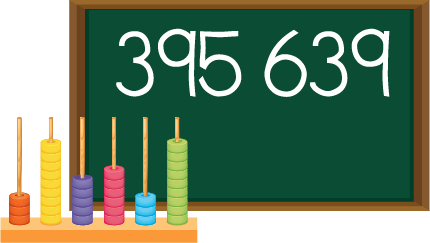
\includegraphics[width=.3\textwidth]{./media/image1.png}
}

\conteudo{
O ábaco da figura é o mais simples e serve somente para representar
números de até 6 ordens. Perceba que cada ordem contém a quantidade de
pedrinhas correspondente ao algarismo que a representa. A primeira haste, da direita, tem 9 pedrinhas verdes, representando o algarismo
nove, da ordem das unidades. A haste logo à esquerda representa a
ordem das dezenas e assim por diante.

%\textless{}https://br.freepik.com/fotos-gratis/garotinho-tendo-uma-sessao-de-terapia-ocupacional\_18036725.htm\#query=\%C3\%A1baco\%20japon\%C3\%AAs\&position=45\&from\_view=search\&track=ais\textgreater{}

\bigskip\noindent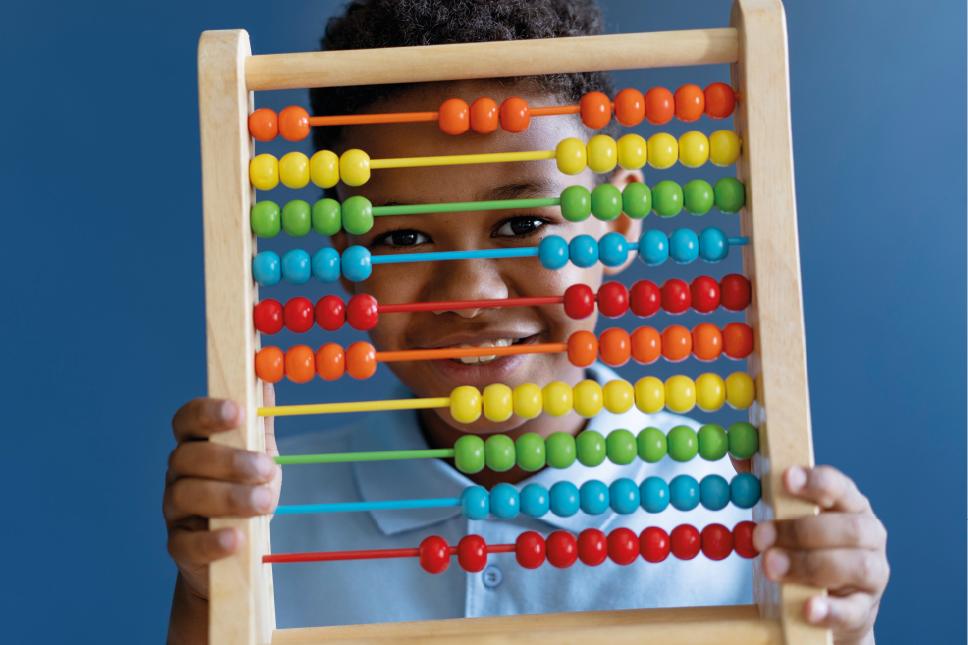
\includegraphics[width=\textwidth]{./media/image2.png}\bigskip

Nessa figura temos um ábaco mais conhecido, onde hastes
horizontais representam as ordens dos números. Para representar o
número zero, posicionamos todas as bolinhas do lado esquerdo. Se
puxarmos duas bolinhas da primeira haste de baixo para a direita, mais
três bolinhas da próxima haste também para a direita, formamos o número
32. Nesse ábaco é possível realizar operações simples, sobrepondo as
pedrinhas que queremos adicionar, por exemplo.

Se possível, leve um ábaco para a sala de aula e demonstre
alguns números aos alunos; ou, então, permita que eles façam alguns.
}

\pagebreak
\colorsec{Atividades}

\num{1} Ligue os números das figuras a seguir, de acordo com o que esses números representam.

%\textless{}https://br.freepik.com/vetores-gratis/ilustracao-de-barcode\_3232987.htm\#query=codigo\%20de\%20barras\&position=2\&from\_view=search\&track=ais; https://br.freepik.com/fotos-premium/nota-de-cem-reais-do-brasil-caindo-sobre-fundo-branco-isolado\_27213030.htm\#query=dinheiro\&position=10\&from\_view=search\&track=sph; https://br.freepik.com/vetores-gratis/podio-do-vencedor-de-esportes-iluminados_1529256.htm#query=podium&position=36&from_view=search&track=sph

\begin{figure}[htpb!]
\centering
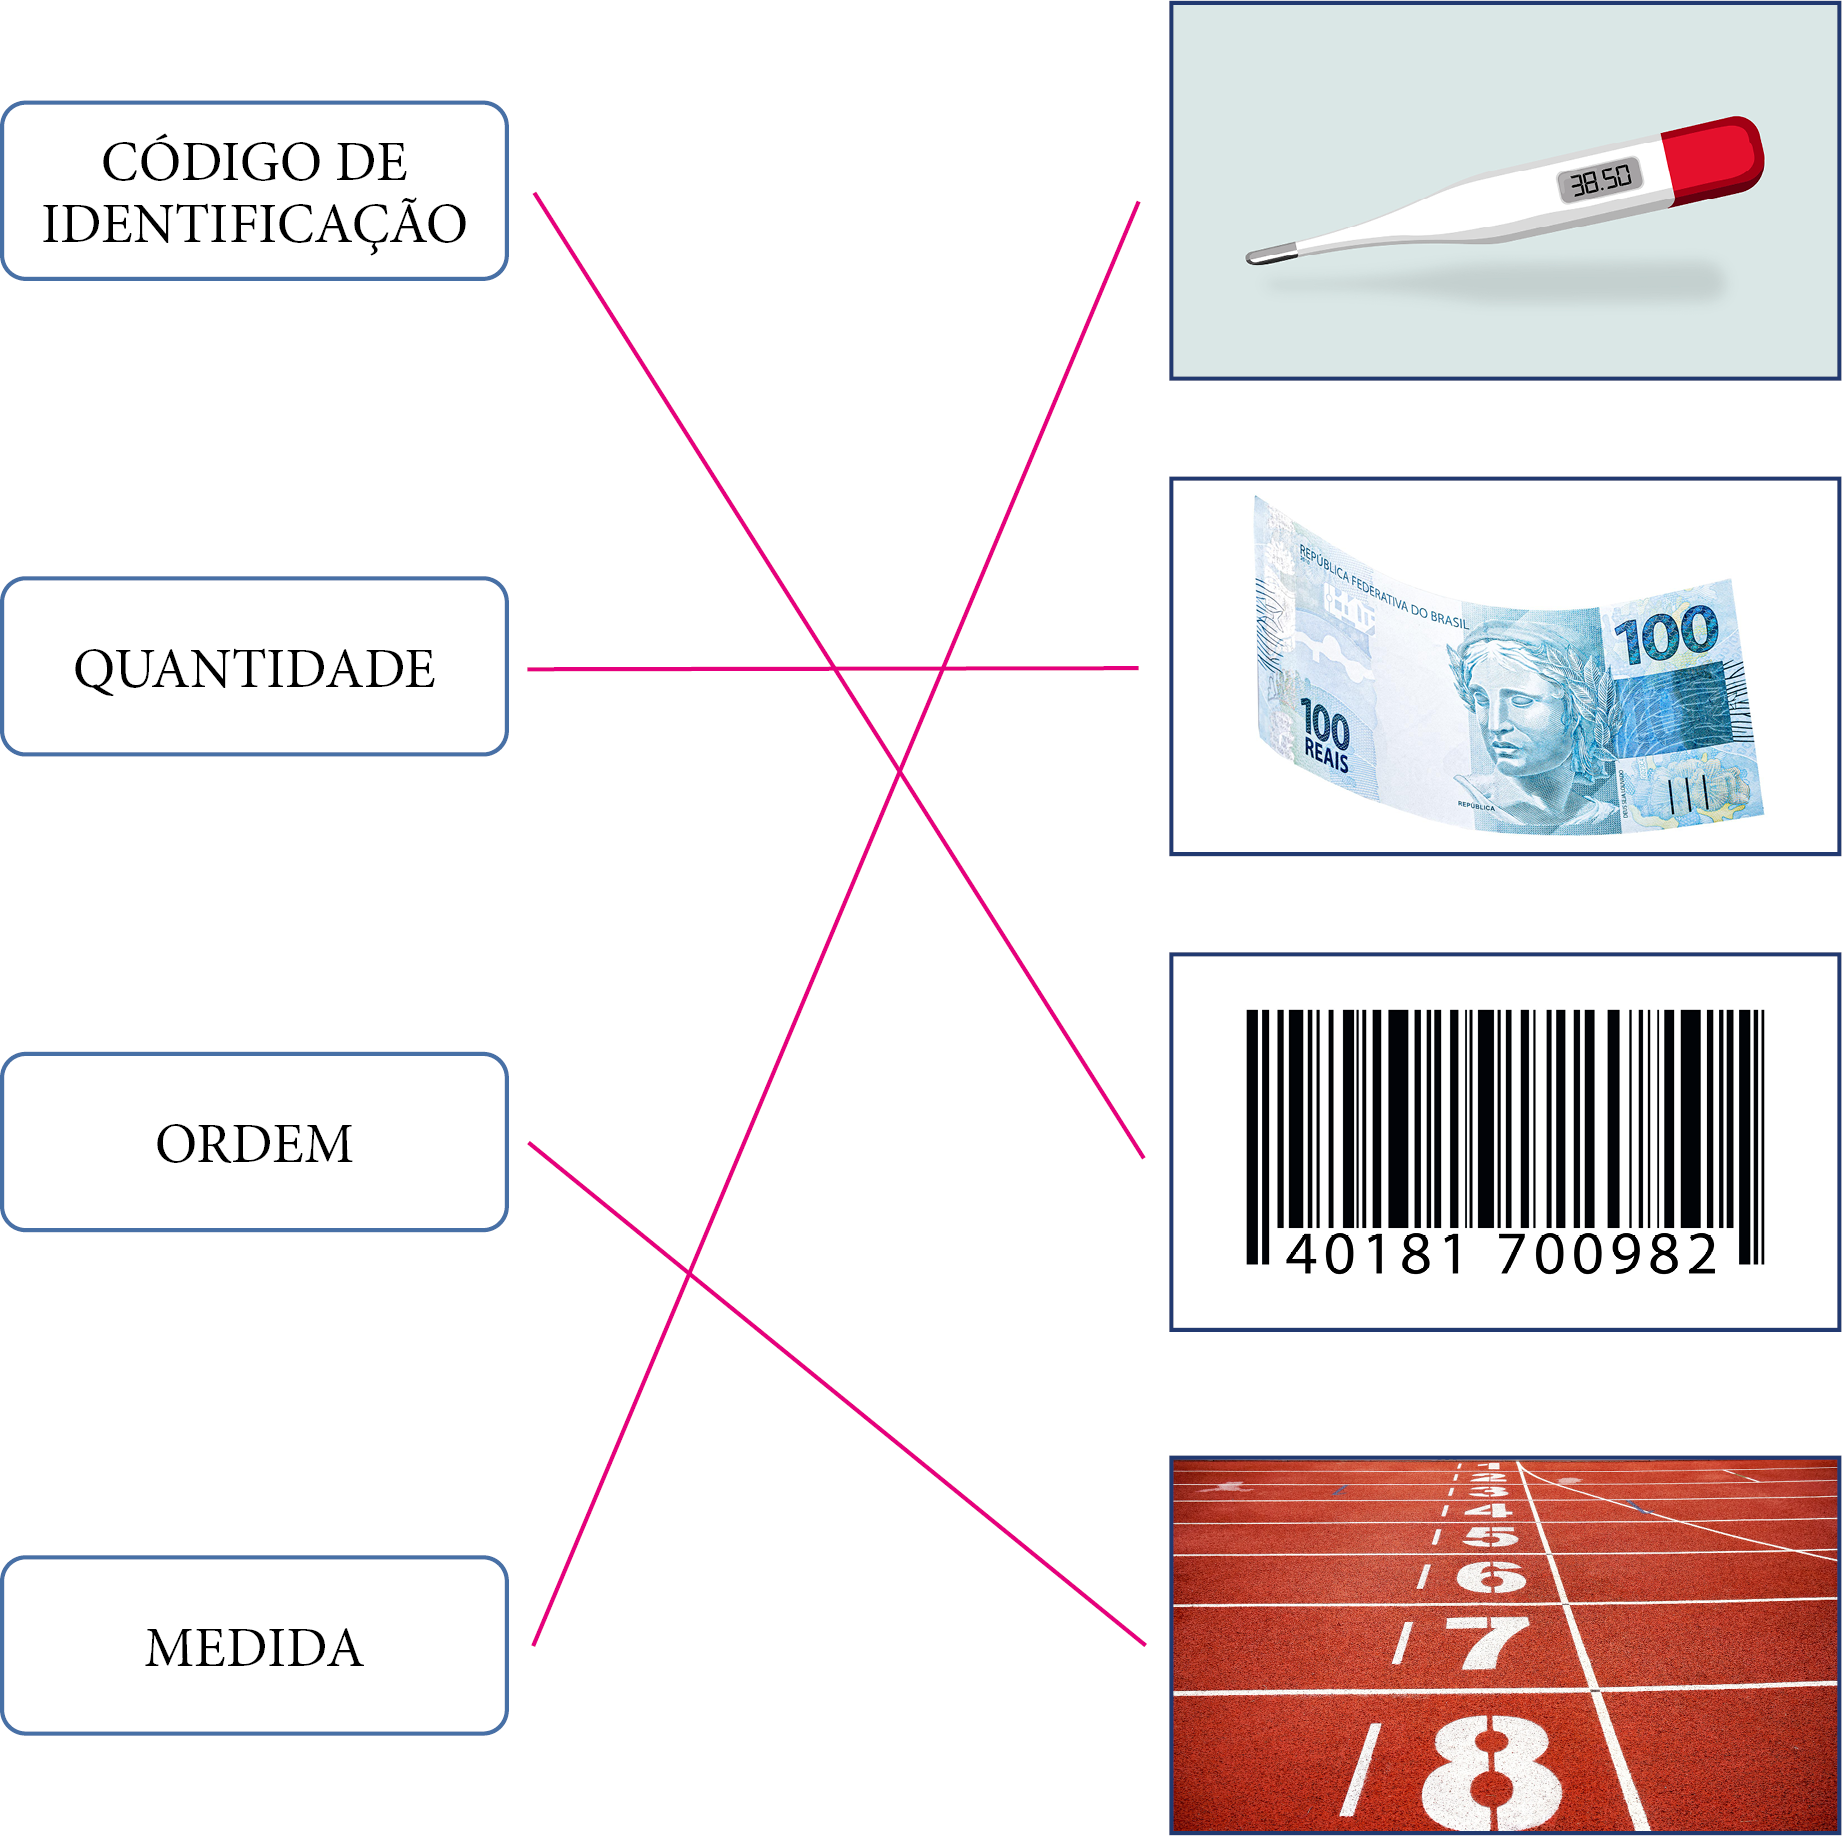
\includegraphics[width=.8\textwidth]{./media/image3.png}
\end{figure}

%\coment{Oriente os alunos a pensarem na função que cada número exerce, nas aplicações em que são apresentados, antes de escolherem a relação.}

\num{2} Pinte o quadrado que contém o 5° número da sequência de números a seguir.
Cuidado! Esses números estão fora da ordem; portanto, você deve
ordená-los primeiro.

\begin{figure}[htpb!]
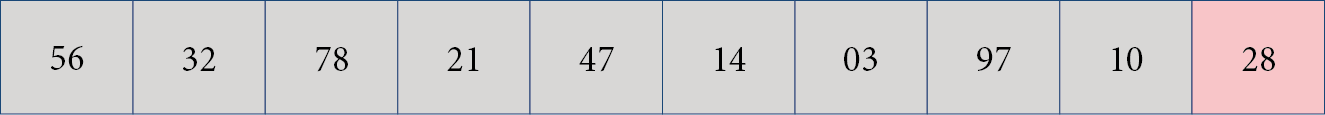
\includegraphics[width=\textwidth]{./media/image4.png}
\end{figure}

%\coment{Oriente os alunos a primeiramente ordenar os números em uma folha separada. Algum aluno pode, afoitamente, pintar o quinto quadradinho.}
\pagebreak
\num{3} Escreva por extenso os números representados nos ábacos. A ordem
é crescente da direita para a esquerda, ou seja, a primeira haste da
direita representa as unidades e assim por diante.

\begin{figure}[htpb!]
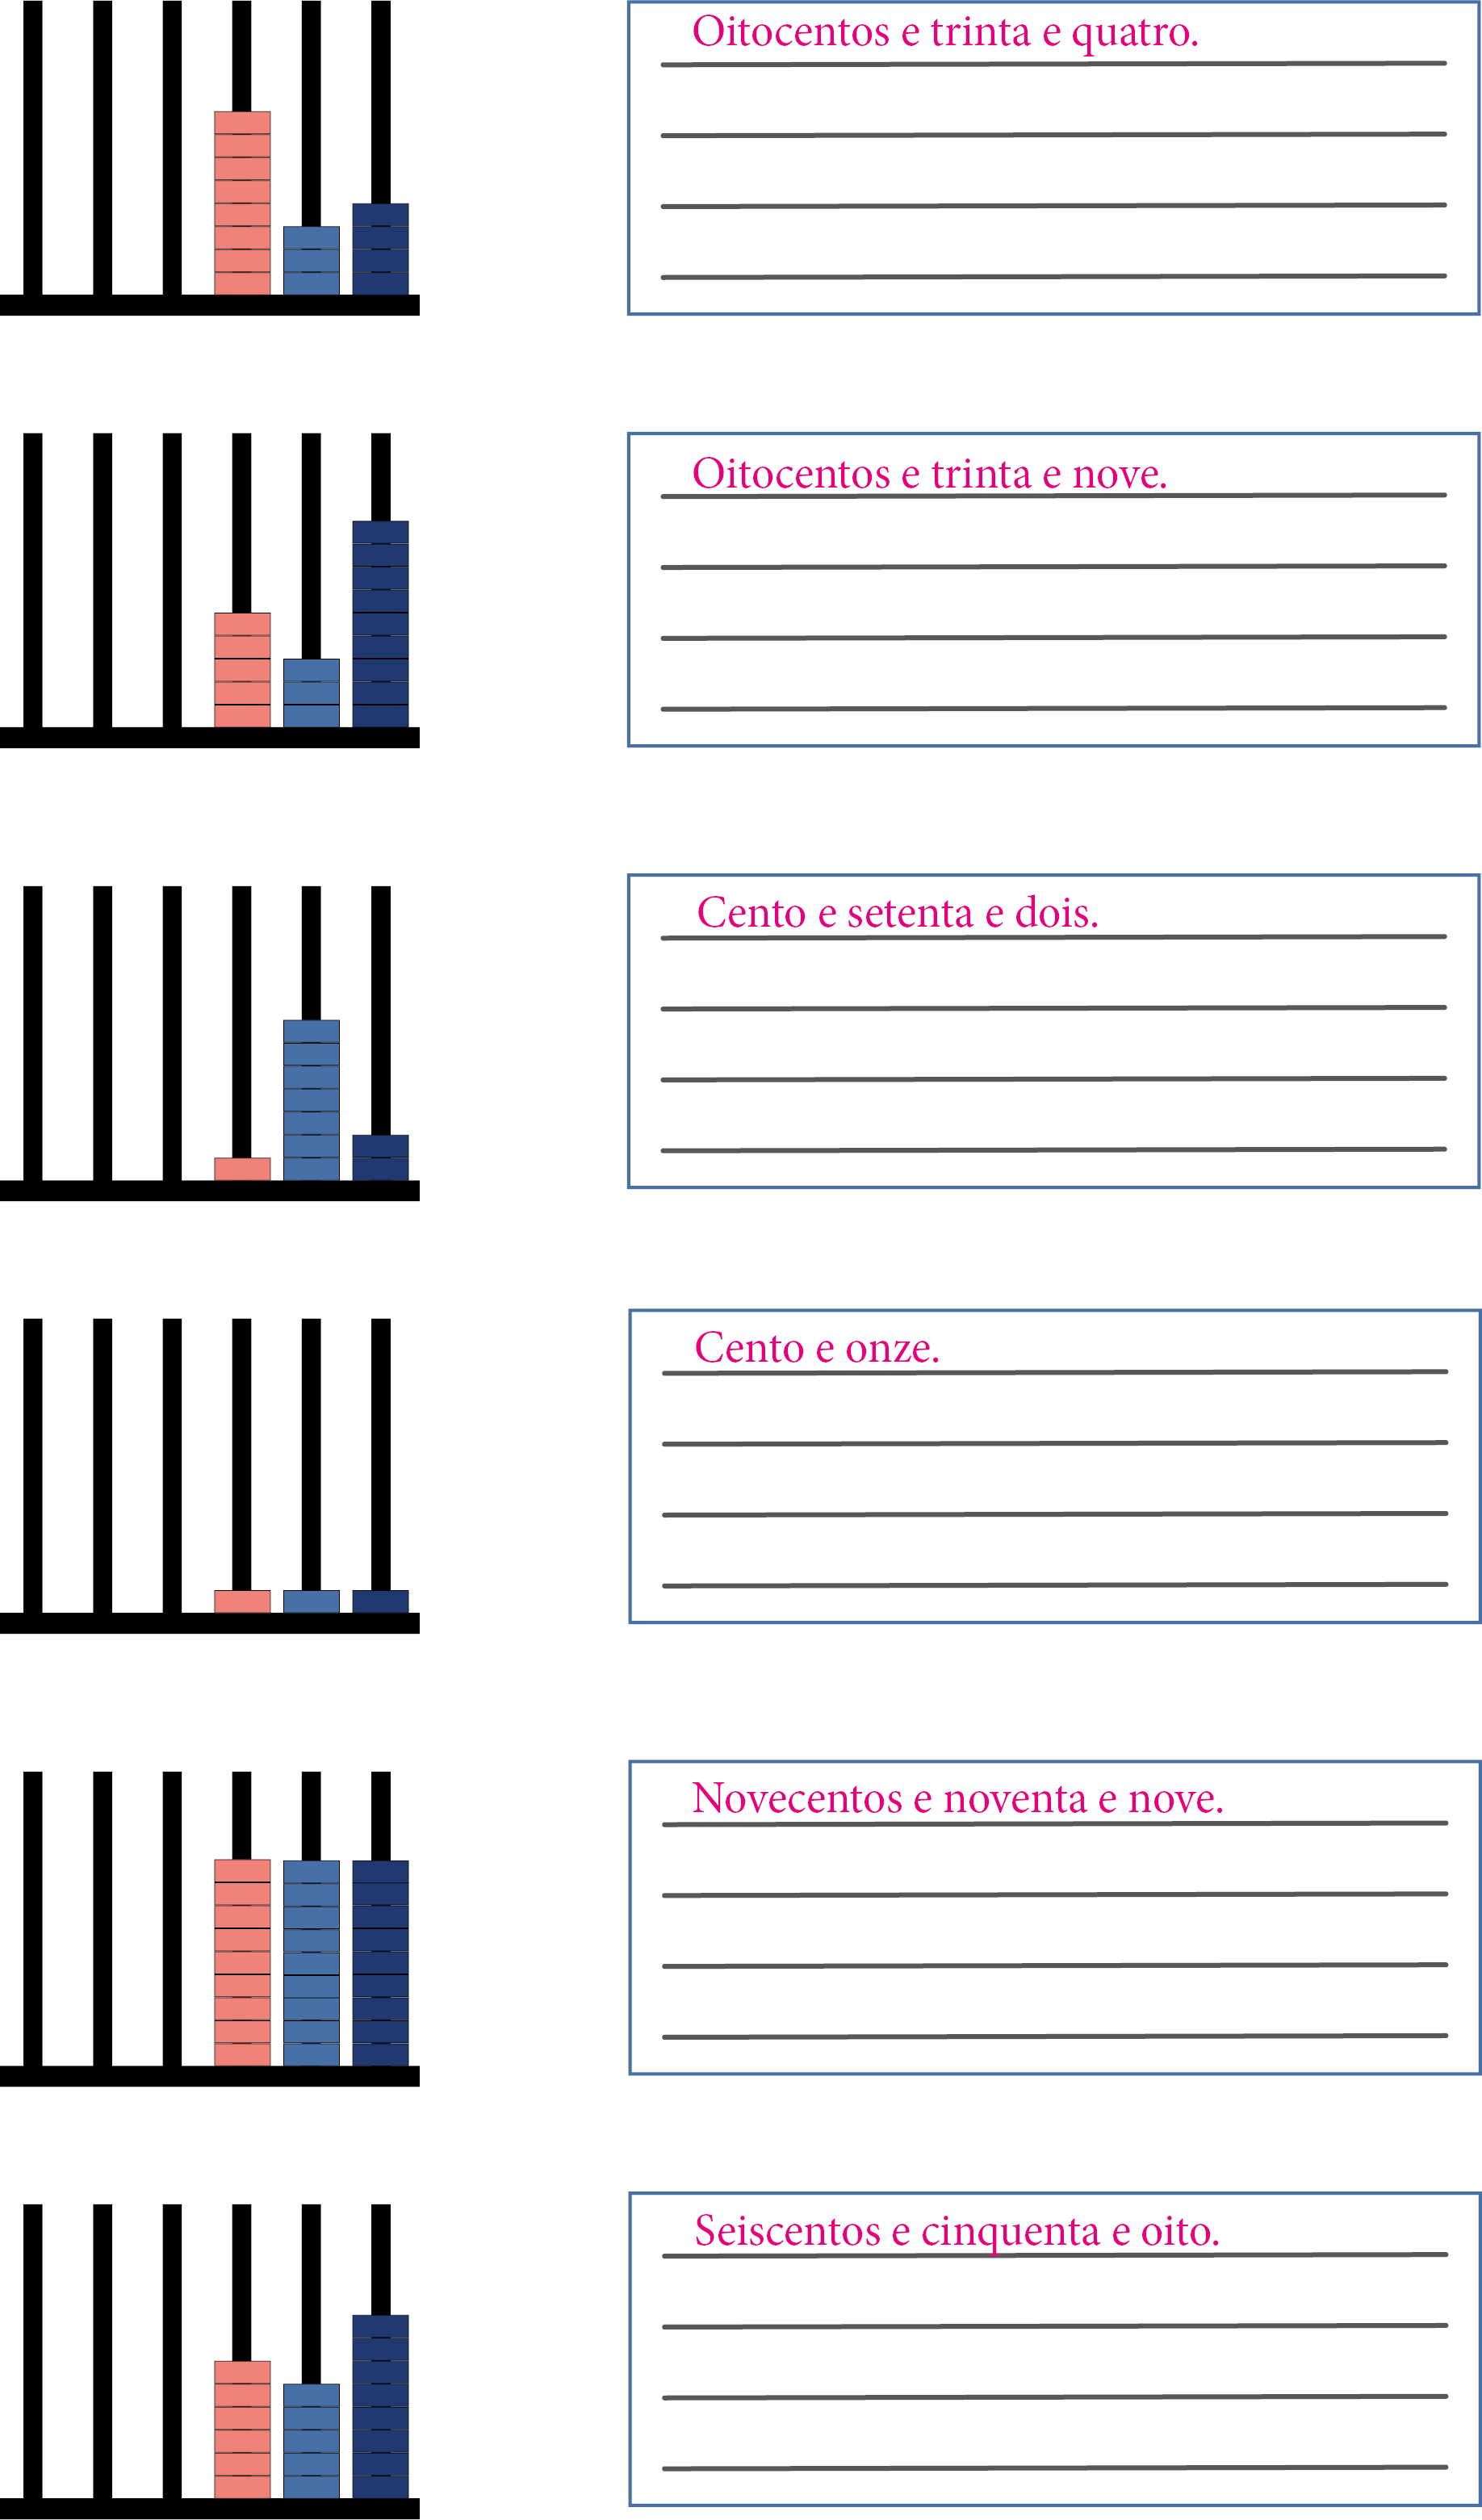
\includegraphics[width=.7\textwidth]{./media/image5.png}
\end{figure}

%\coment{Oriente os alunos a não escreverem os algarismos, mas sim a escreverem os números por extenso, em língua portuguesa.}
\pagebreak

\num{4} Ordene os números representados nos ábacos, preenchendo os
números nos quadros abaixo das letras. Depois, ordene as letras no
quadro das posições.

\begin{figure}[htpb!]
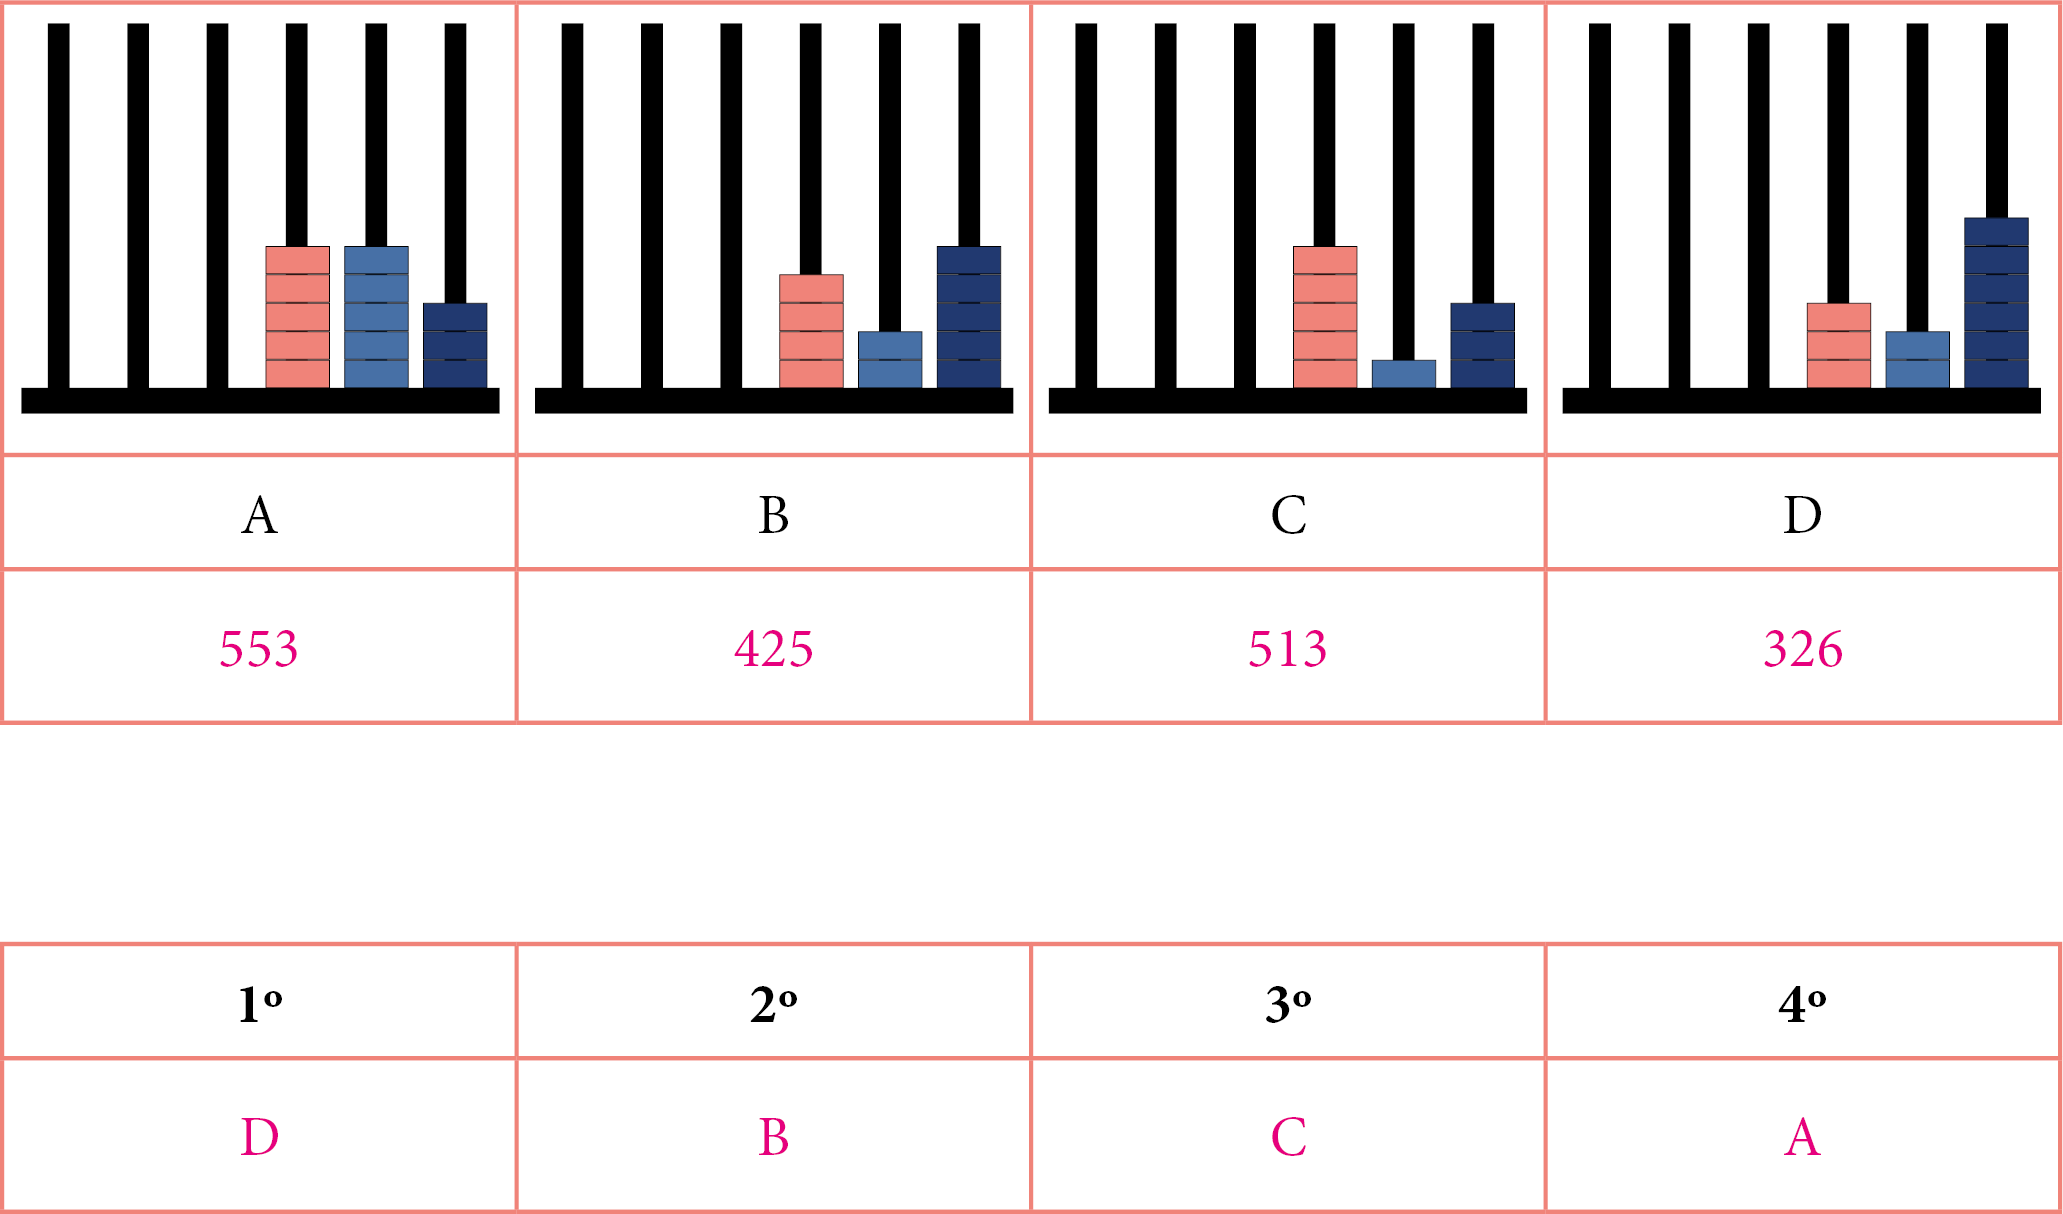
\includegraphics[width=\textwidth]{./media/image6.png}
\end{figure}

%\coment{Oriente os alunos a descobrirem os números, antes de ordená-los.}


\num{5} É dada a seguinte sequência numérica: 236, 541, 698, 147, 852 e 321. Pinte os
ábacos a seguir, ordenando essa sequência corretamente, de forma
decrescente.

\begin{figure}[htpb!]
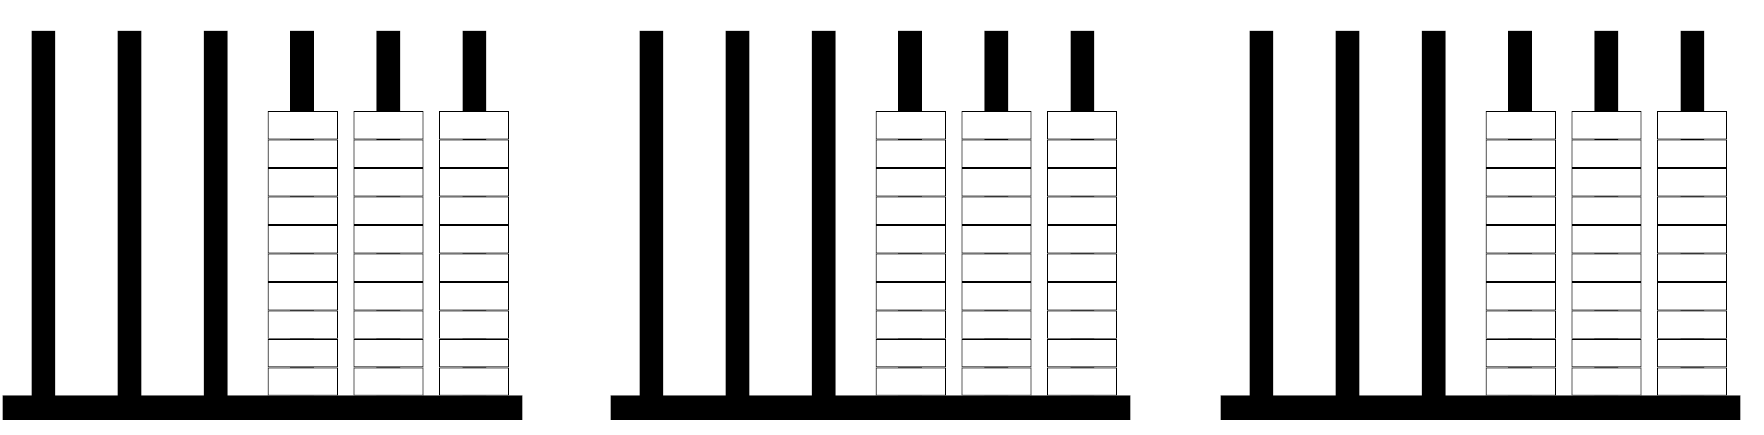
\includegraphics[width=\textwidth]{./media/image7b.png}
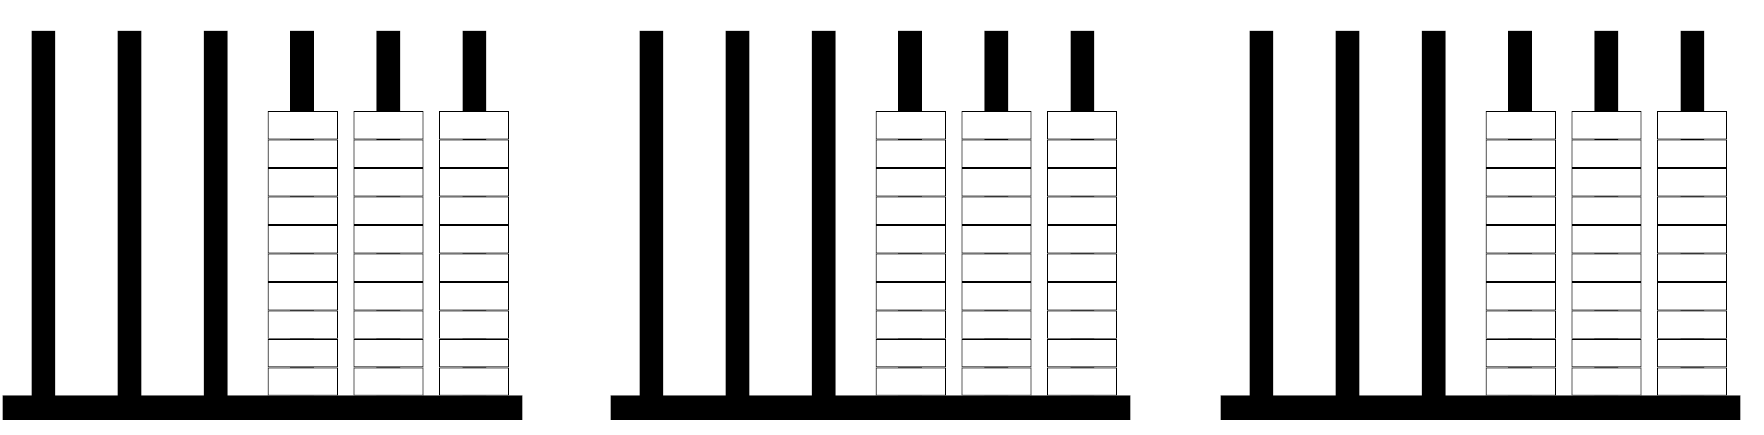
\includegraphics[width=\textwidth]{./media/image7b.png}
\end{figure}

\pagebreak

%\coment{A sequência correta, ordenada de forma decrescente, é: 852, 698, 541, 321, 236 e 147.}
%Oriente os alunos a preencherem o ábaco, considerando a primeira coluna à direita, como representante da ordem das unidades.}

\num{6} Descubra a charada. Eu sou um algarismo. Se adicionarem o meu valor à
segunda ordem no número 3~927, da direita para a esquerda, os números das próximas
ordens serão mudados. Que algarismo eu sou?

%\textless{}https://br.freepik.com/vetores-gratis/colecao-de-numeros-dos-desenhos-animados-com-personagens\_2310814.htm\#query=n\%C3\%BAmeros\%20malucos\%20abra\%C3\%A7ado\&position=34\&from\_view=search\&track=ais\textgreater{}

\begin{figure}[htpb!]
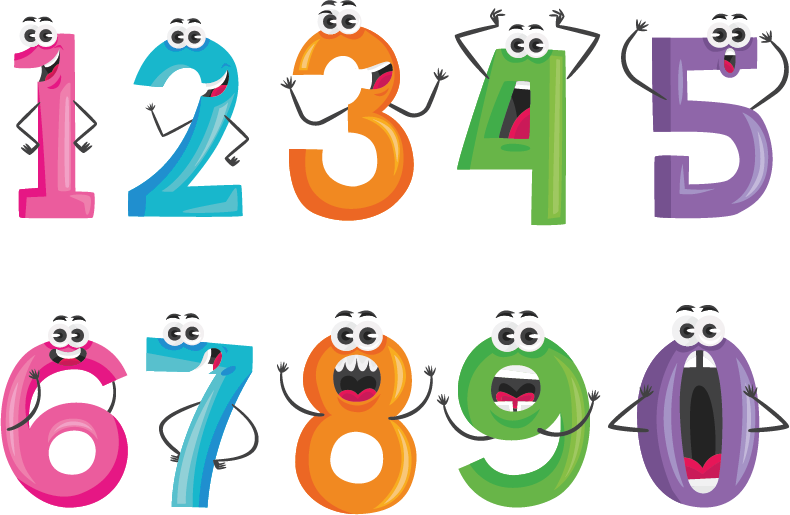
\includegraphics[width=\textwidth]{./media/image8.png}
\end{figure}


\reduline{O aluno deve perceber que, se ele somar o algarismo 8 à
ordem das dezenas, o número obtido será o 4007; logo, as ordens das
centenas e milhares terão seus algarismos modificados. Porém, o
algarismo da ordem das unidades continuará o mesmo.\hfill}
\linhas{3}

\pagebreak
\num{7} Dê exemplos de como os números podem ser usados em cada uma das
situações.

\begin{figure}[htpb!]
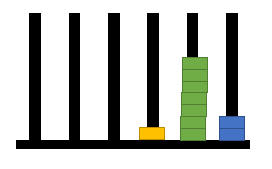
\includegraphics[width=\textwidth]{./media/image9.png}
\end{figure}

%\coment{Tente estimular os próprios alunos a citarem diferentes exemplos. Caso, porém, eles não consigam fazê-lo de forma autônoma, ajude-os, mostrando você mesmo a eles os exemplos.}

\pagebreak

\num{8} Jorge estava correndo uma maratona em sua cidade. Ele começou a corrida
na posição 63. Na primeira metade da corrida, ele ultrapassou 18
competidores. Na segunda metade, o cansaço chegou; logo, ele foi
ultrapassado por 5 desses competidores que ele havia ultrapassado antes.
Mas, perto do fim da corrida, Jorge juntou forças, começou a correr como
nunca e ultrapassou mais 25 corredores, antes de cruzar a linha de
chegada. Olhe a tabela e indique qual foi o prêmio de Jorge.

\begin{figure}[htpb!]
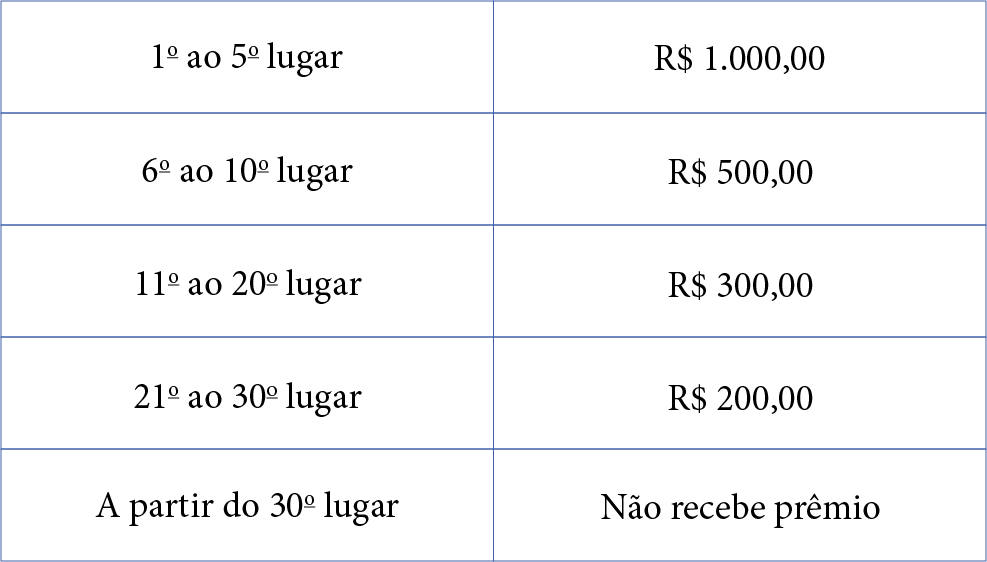
\includegraphics[width=\textwidth]{./media/image10.png}
\end{figure}

\coment{Jorge chegou à metade da corrida em 45° (63 - 18).

Na segunda metade, ficou em 50° (45 + 5).

No finalzinho, ele cruzou a linha em 25° (50 - 25).

Logo, o prêmio foi de de R\$ 200,00.}

\pagebreak
\num{9} Indique quais dos números a seguir estão no caça-palavras. Pinte
as bolas que contêm esses números.

\begin{figure}[htpb!]
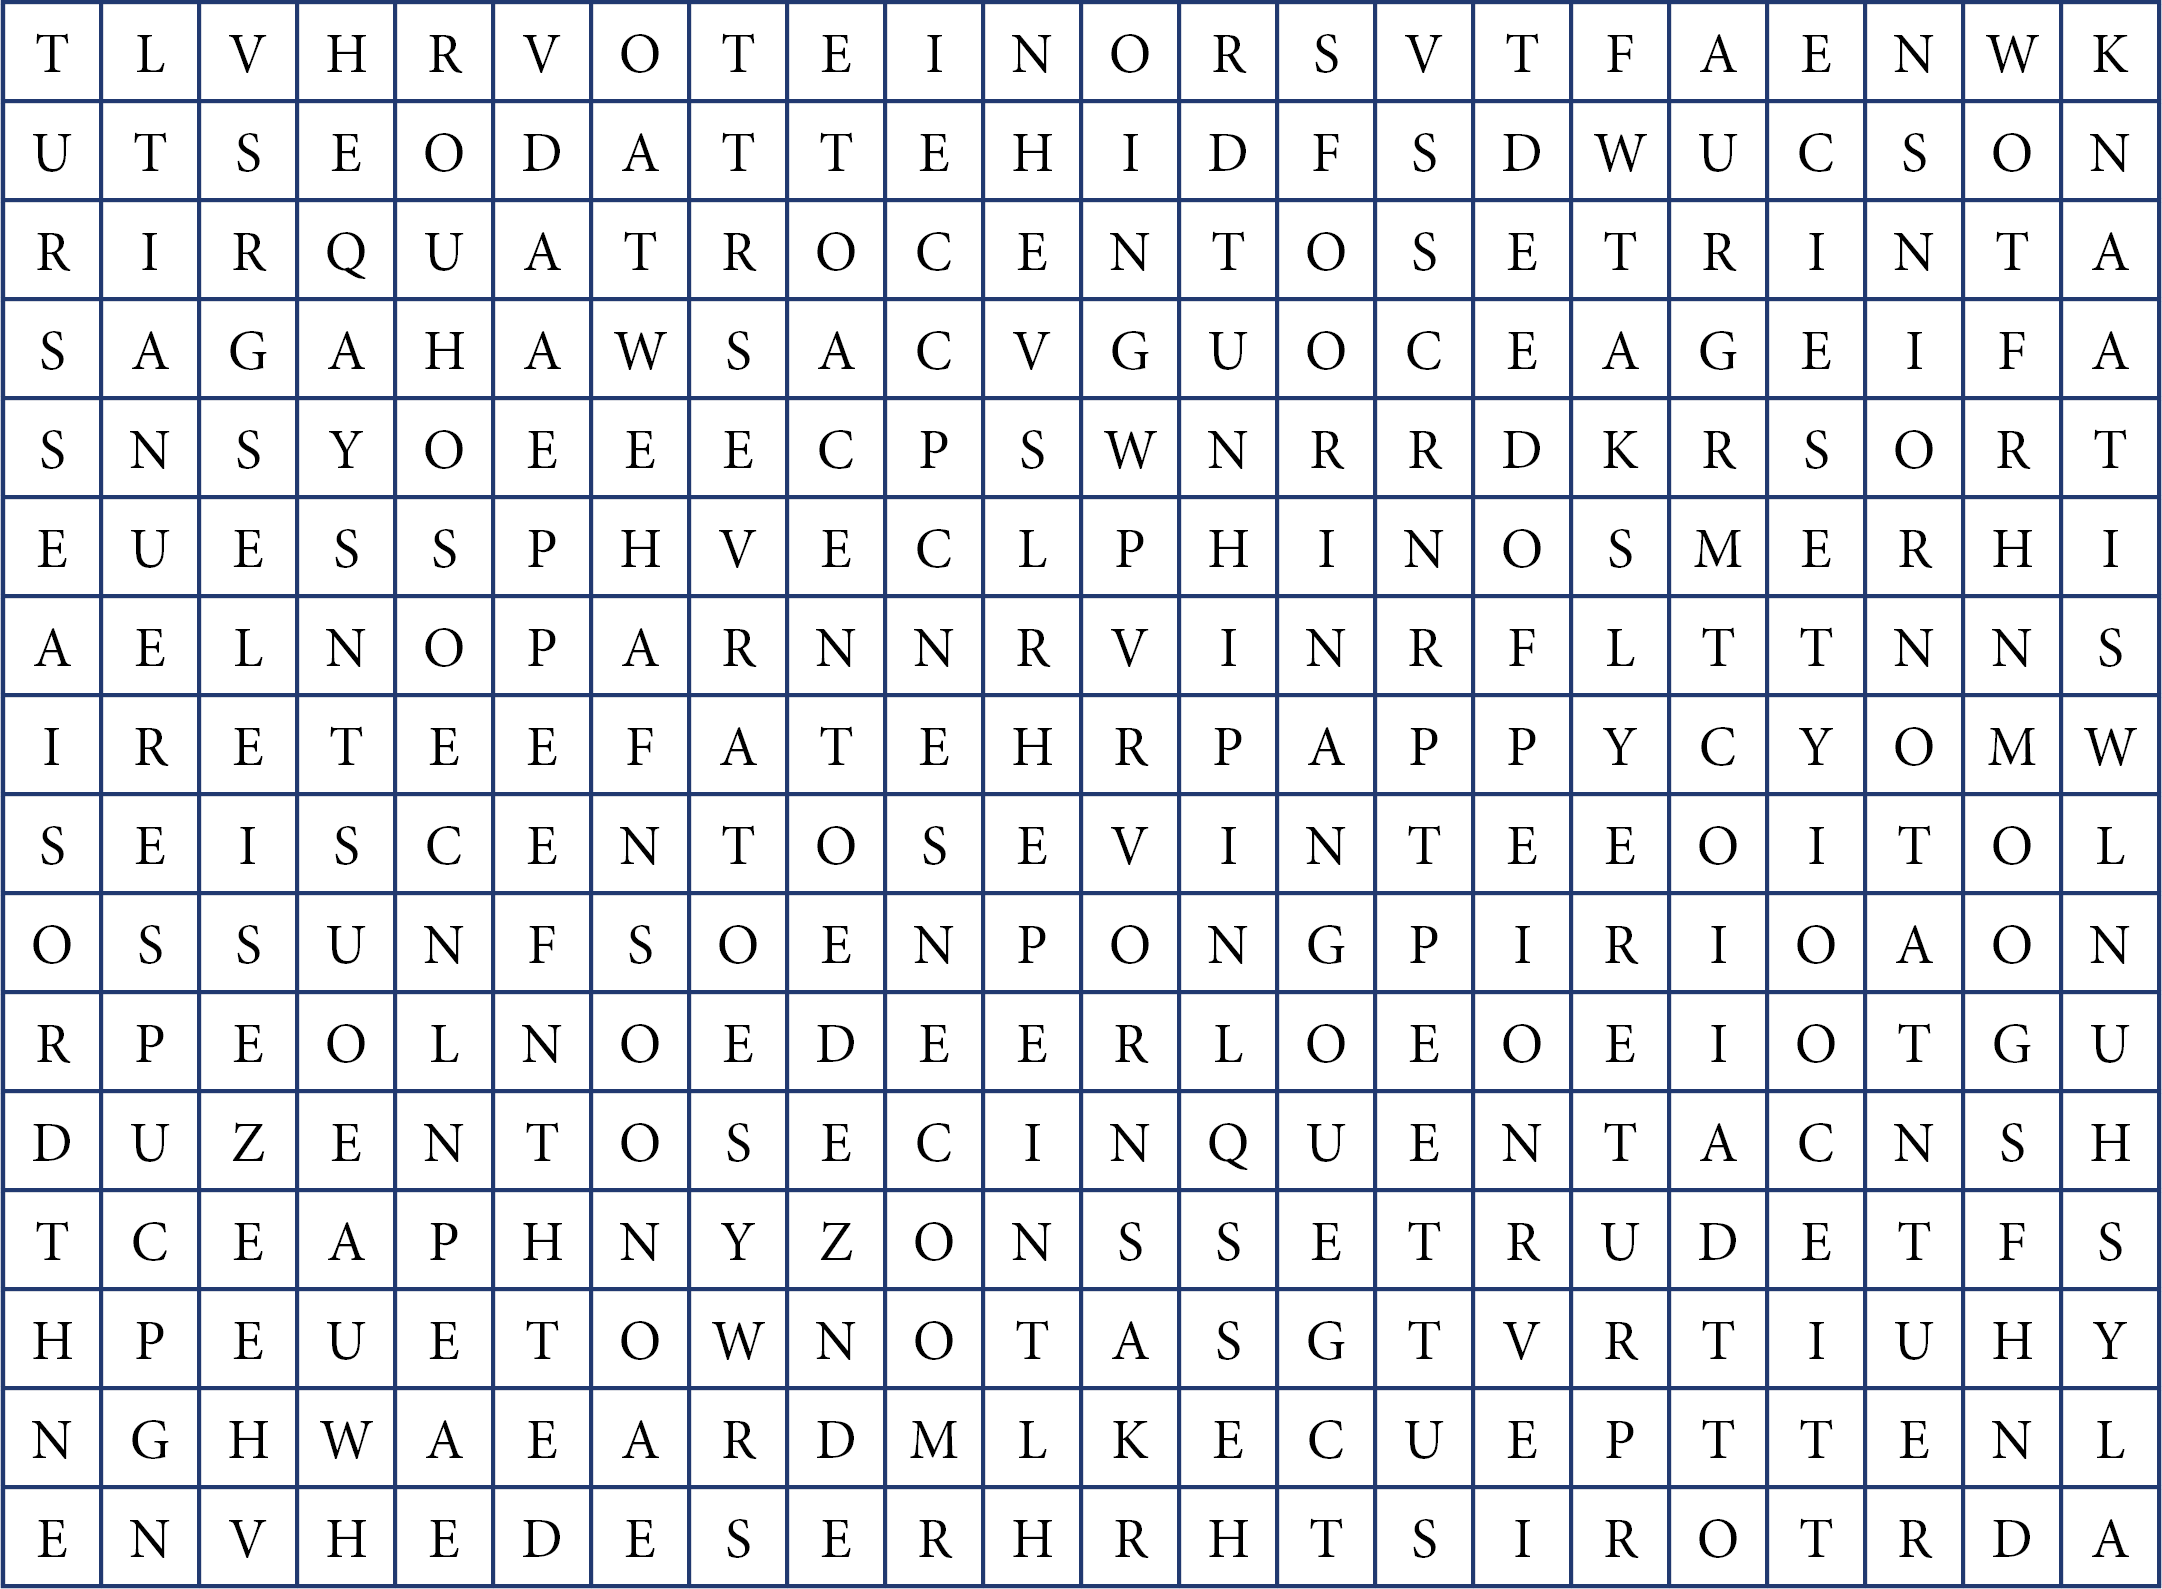
\includegraphics[width=\textwidth]{./media/image11.png}
\end{figure}

\begin{figure}[htpb!]
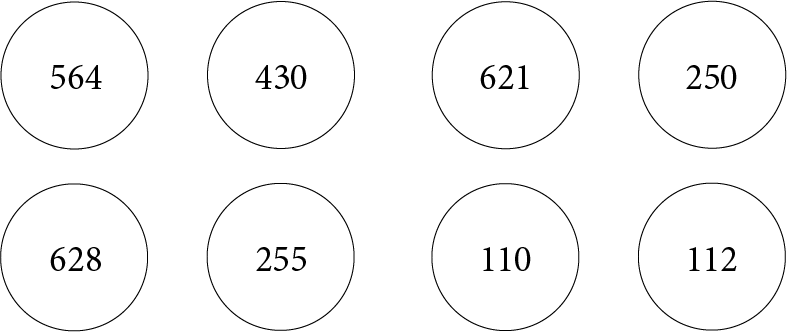
\includegraphics[width=\textwidth]{./media/image12.png}
\end{figure}

\coment{Os números encontrados são: 628, 430, 110 e 250.}

\pagebreak
\num{10} Alinhe os estabelecimentos na reta numérica. Escreva o nome dos
estabelecimentos nos quadrados correspondentes, depois de ler o texto.

\begin{figure}[htpb!]
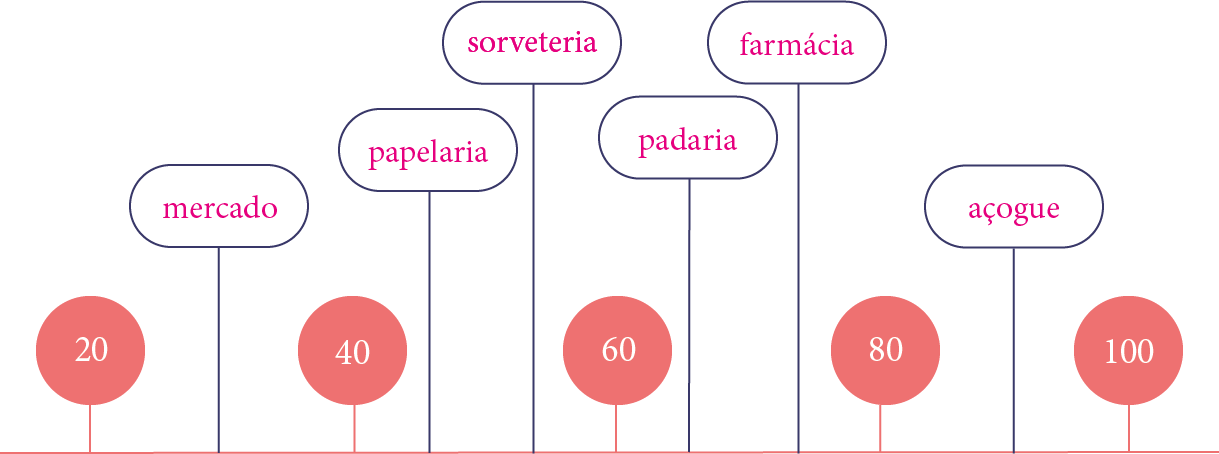
\includegraphics[width=\textwidth]{./media/image14.png}
\end{figure}

%\coment{Uma padaria fica entre os números 60 e 100 de determinada rua. Já a farmácia fica entre a padaria e o açougue. A sorveteria fica no número 46, logo após a papelaria. O mercado fica antes da papelaria.}

% \num{11} Analise os números e preencha a tabela com as informações pedidas.

% \begin{figure}[htpb!]
% \centering
% 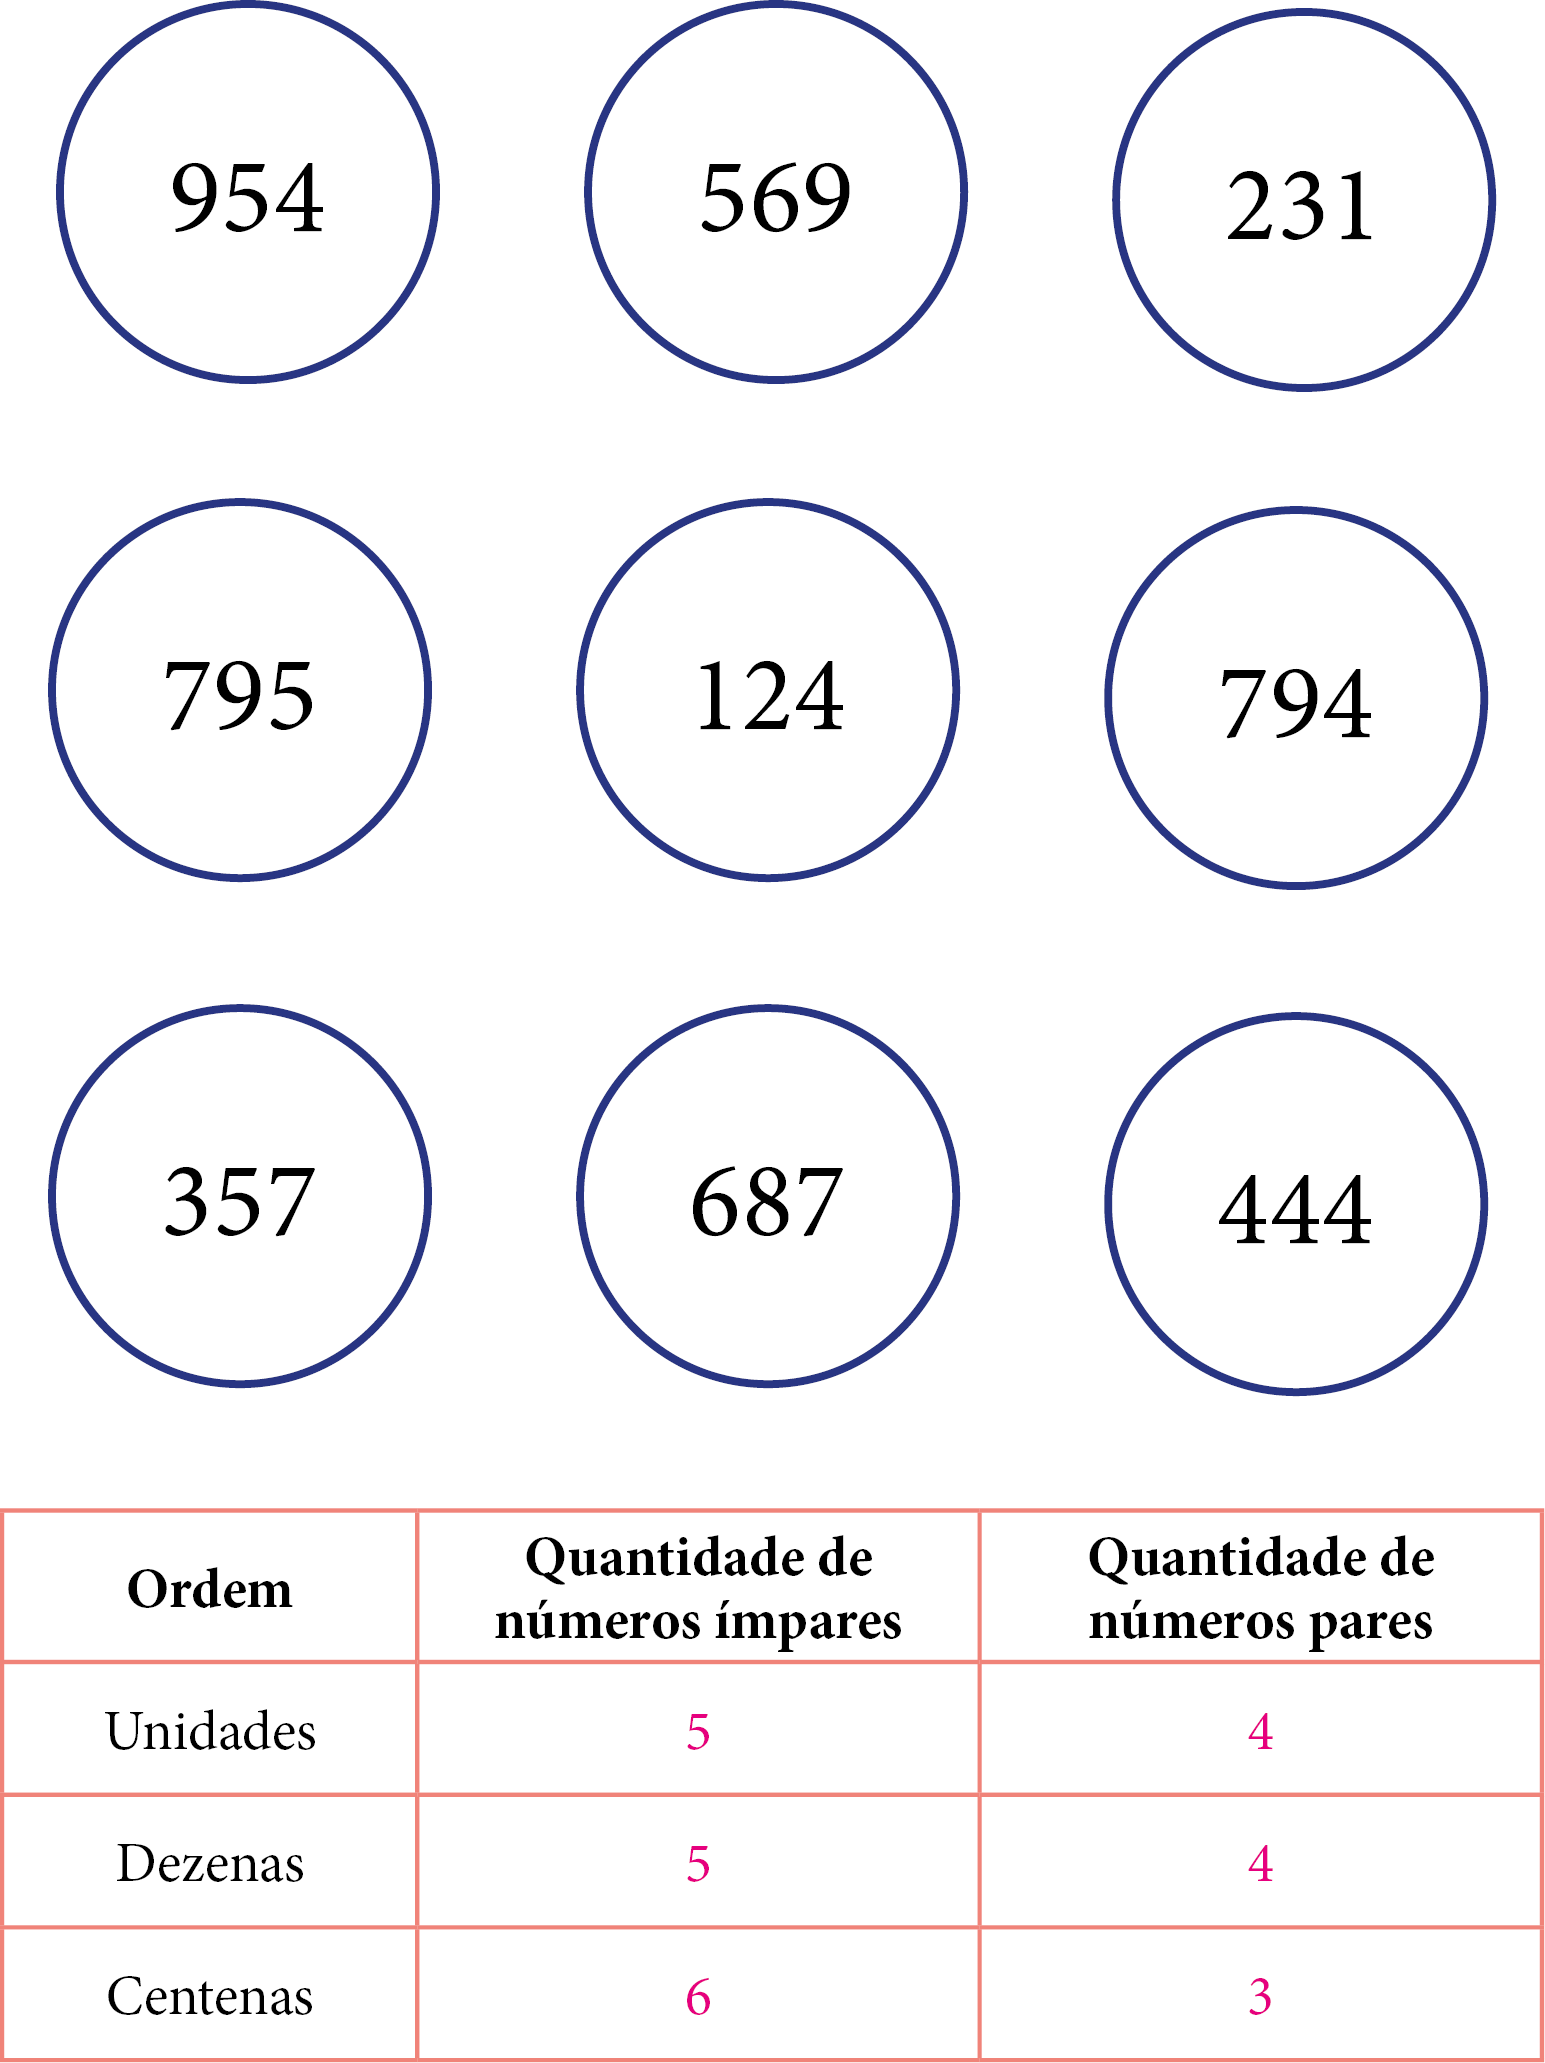
\includegraphics[width=.5\textwidth]{./media/image15.png}
% \end{figure}

%\coment{Oriente os alunos a contarem a quantidade de números pares e ímpares em cada ordem de cada número apresentado nas bolas.}

\colorsec{Treino}

\num{1} A senha do cartão de crédito é um número que indica um(a):

\begin{escolha}
\item Código de identificação.

\item Medida.

\item Quantidade.

\item Ordem.
\end{escolha}

\num{2} Indique qual é o 30° número par entre os números 0 e 100.

\begin{escolha}
\item 30

\item 40

\item 60

\item 90
\end{escolha}

\pagebreak
\num{3} Qual dos ábacos a seguir representa um número com algarismo ímpar na ordem
das dezenas.

\begin{figure}[htpb!]
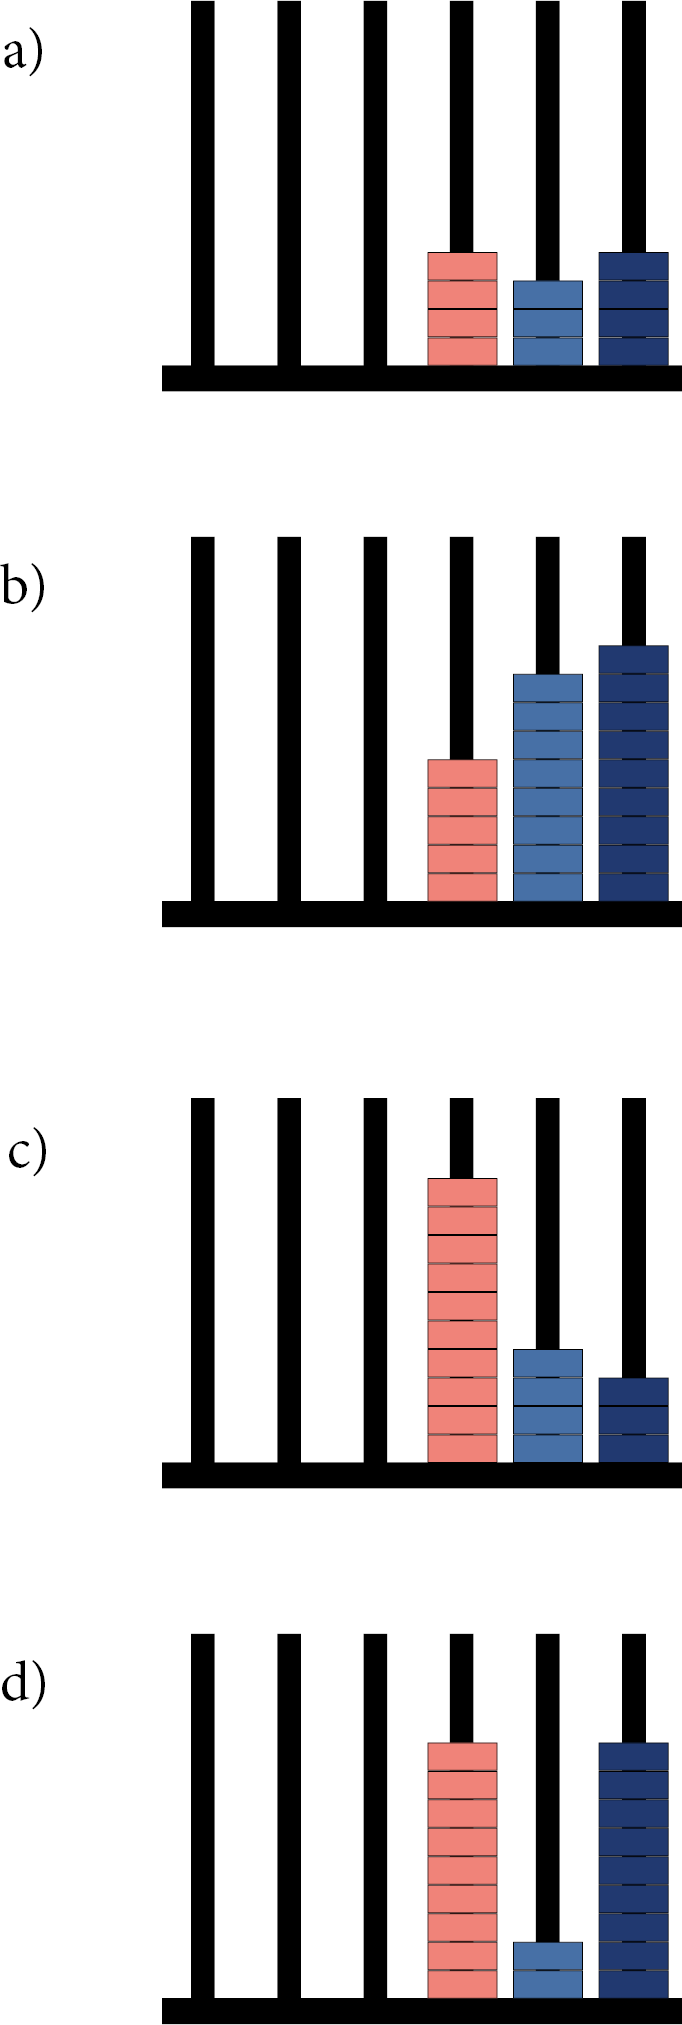
\includegraphics[scale=1]{./media/image16.png}
\end{figure}

\chapter{Virando figurinhas}
\markboth{Módulo 2}{}


%\coment{Neste módulo, vamos desenvolver a habilidade de desenvolvimento de cálculos, tanto no sentido de escolher a melhor estratégia quanto no sentido de resolver o problema. Faremos essa abordagem de forma abstrata, mas também de forma contextualizada, com o fim de desenvolver nos alunos a motivação para resolverem problemas reais. }

\colorsec{Habilidades do SAEB}

\begin{itemize}
\item Calcular o resultado de adições e subtrações, envolvendo números naturais de até 3 ordens.

\item Compor ou decompor números naturais de até 3 ordens por meio de diferentes adições.

\item Resolver problemas de adição ou de subtração, envolvendo números
naturais de até 3 ordens, com os significados de juntar, acrescentar, separar ou retirar.
\end{itemize}

\colorsec{Habilidades da BNCC}

\begin{itemize}
\item EF02MA04, EF02MA06.
\end{itemize}

\conteudo{
\begin{wrapfigure}{r}{.5\textwidth}
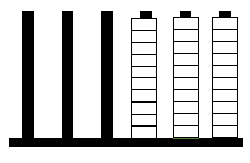
\includegraphics[width=.5\textwidth]{./media/image17.png}
\end{wrapfigure}

Você já jogou bafo? Ou, então, talvez em sua cidade essa brincadeira se
chame tapão! Se já jogou, qual é o seu recorde de virada de figurinhas?

Se nunca ouviu falar, é um jogo em que você tem que deslocar a
maior quantidade de ar possível, fazendo com que um bolo de figurinhas
seja virado. Quem virar mais figurinhas ganha o jogo, e ainda fica com
as figurinhas do seu oponente. A turma toda se junta para competir. 
}

\conteudo{Mas
todos precisam ter certeza de quantas figurinhas possuem, para que
ninguém fique com as figurinhas de ninguém por engano. Joel tinha 63
figurinhas de jogadores de futebol, Cristiano tinha mais 43, Eduardo
tinha mais 52 e Ricardo, 81. Eles resolveram apostar tudo e ir
competindo até ver quem ficava com mais figurinhas no final do jogo. Mas,
para isso, eles precisavam adicionar as figurinhas de cada um. Como
eram muitas figurinhas, resolveram fazer pela ordem dos números.
Observe o quadro a seguir.\bigskip

\noindent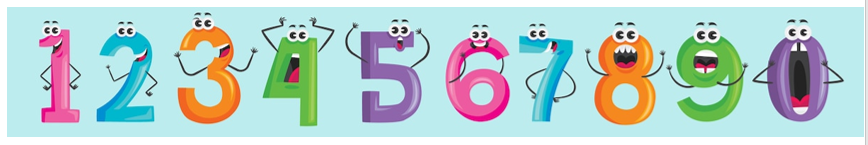
\includegraphics[width=\textwidth]{./media/image18.png}\bigskip

Os meninos resolveram separar os números das quantidades de figurinhas
pela ordem. Descobriram que suas figurinhas adicionadas somam 9 unidades
e 23 dezenas. Logo, pensaram: Se temos 23 dezenas, e cada 10 dezenas
formam uma centena, então temos 2 centenas, 3 dezenas e 9 unidades.
Pensando assim, os amigos encontraram a quantidade total de figurinhas, que é de 239.
}

\pagebreak
\colorsec{Atividades}

\num{1} Complete o quadro a seguir.

\begin{figure}[htpb!]
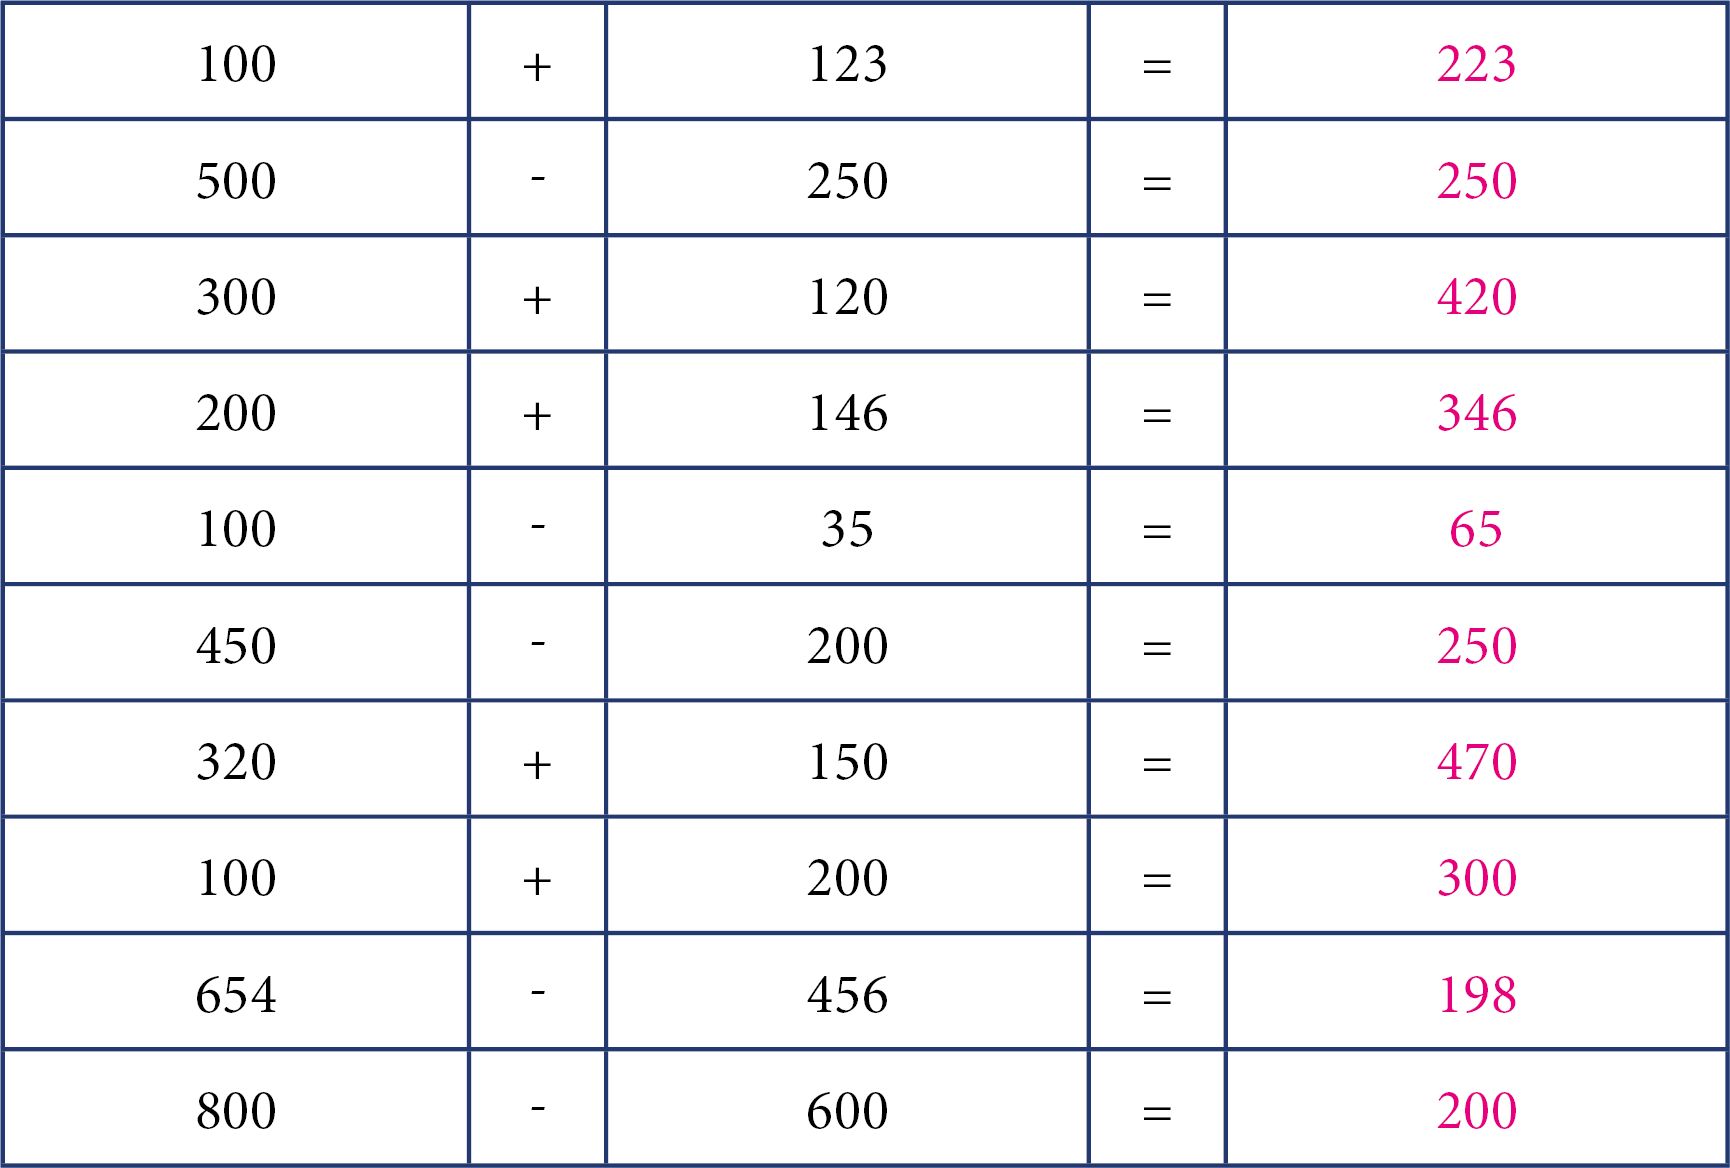
\includegraphics[width=\textwidth]{./media/image19.png}
\end{figure}

\pagebreak
\num{2} Vamos caçar números? Pinte o resultado das adições e subtrações a seguir,
conforme a cor. Se o número representar o resultado de uma adição, deverá ser pintado de amarelo. Se, por outro lado, ele representar o resultado de uma subtração, ele deverá ser pintado de azul.

\begin{figure}[htpb!]
\centering
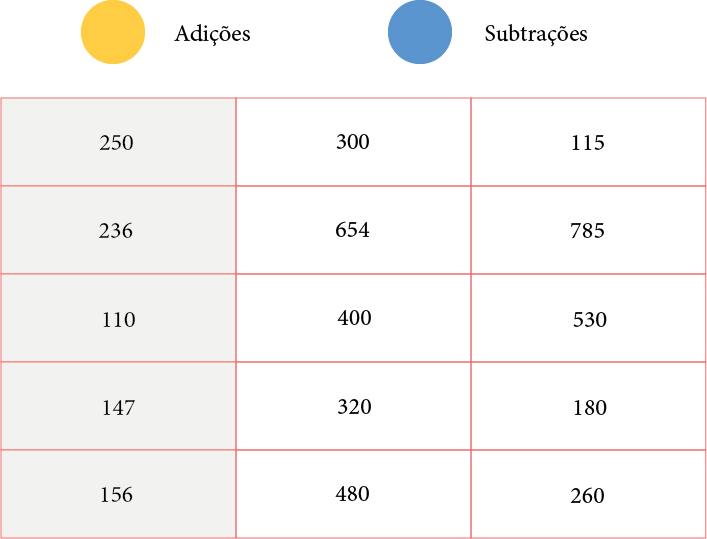
\includegraphics[width=\textwidth]{./media/image20.png}
\end{figure}

%\textless{}Inserir uma linha na frente de cada conta abaixo.\textgreater{}

\begin{minipage}{.5\textwidth}
\begin{escolha}
\item 190 -- 10 = 180

\item 125 + 125 = 250

\item 900 -- 115 = 785

\item 100 + 15 = 115

\item 500 +154 = 654

\item 100 + 10 = 110

\item 300 - 153 = 147

\item 600 -- 200 = 400

\item 600 -- 300 = 300

\item 700 - 220 = 480

\item 250 + 280 = 530

\item 134 + 22 = 156

\item 300 + 20 = 320

\item 190 + 70 = 260

\item 400 - 164 = 236
\end{escolha}
\end{minipage}
\sidetext{Os números 250, 115, 654, 110, 530, 156, 320 e 260 devem ser pintados de amarelo, porque são resultados de adições. Já os números 180, 785, 147, 400, 300, 480 e 236 devem ser pintados de azul, por representarem subtrações.}

\num{3} Escreva pelo menos duas formas de compor os números a seguir, utilizando
três parcelas, apenas por meio de adição. Para isso, siga o modelo.

%\textless{}Inserir uma linha na frente de cada número.\textgreater{}

\begin{mdframed}[linewidth=2pt,linecolor=azul!20,backgroundcolor=azul!20,roundcorner=2pt]
500: 250 + 125 + 125 ou 200 + 150 + 150.
\end{mdframed}

\begin{itemize}
\item 650: \reduline{Sugestão de resposta: 600 + 30 + 20 ou 500 + 100 + 50\hfill}

\item 160: \reduline{Sugestão de resposta: 80 + 70 + 10 ou 50 + 50 + 60\hfill}

\item 236: \reduline{Sugestão de resposta: 200 + 35 + 1 ou 100 + 35 + 101\hfill}

\item 129: \reduline{Sugestão de resposta: 100 + 20 + 9 ou 127 + 1 + 1\hfill}

\item 450: \reduline{Sugestão de resposta: 150 + 150 + 150 ou 300 + 100 + 50\hfill}

\item 975: \reduline{Sugestão de resposta: 900 + 70 + 5 ou 375 + 300 + 300\hfill}

\item 135: \reduline{Sugestão de resposta: 100 + 30 + 5 ou 50 + 50 + 35\hfill}

\item 740: \reduline{Sugestão de resposta: 350 + 350 + 40 ou 400 + 300 + 40\hfill}
\end{itemize}

%\coment{Os alunos poderão compor os números da forma que quiserem. Certifique-se de que eles usem pelo menos três parcelas e de que a adição esteja correta. É dado um exemplo no primeiro número.}

\num{4} Escreva pelo menos duas formas de compor os mesmos números a seguir,
utilizando três parcelas, utilizando somente a subtração. Para isso, siga o modelo.

%\textless{}Inserir uma linha na frente de cada número.\textgreater{}

\begin{mdframed}[linewidth=2pt,linecolor=azul!20,backgroundcolor=azul!20,roundcorner=2pt]
500: 900 -- 200 -- 200 ou 600 -- 50 -- 50.
\end{mdframed}

\begin{itemize}
\item 650: \reduline{Sugestão de resposta: 1000 -- 300 -- 50 ou 900 -- 150 -- 100\hfill}

\item 160: \reduline{Sugestão de resposta: 300 -- 100 -- 40 ou 200 -- 20 -- 20\hfill}

\item 236: \reduline{Sugestão de resposta: 400 -- 100 -- 64 ou 300 -- 50 -- 14\hfill}

\item 129: \reduline{Sugestão de resposta: 200 -- 70 -- 1 ou 250 -- 71 -- 50\hfill}

\item 450: \reduline{Sugestão de resposta: 900 -- 400 -- 50 ou 500 -- 30 -- 20\hfill}

\item 975: \reduline{Sugestão de resposta: 1000 -- 20 -- 5 ou 2000 -- 1000 -- 25\hfill}

\item 135: \reduline{Sugestão de resposta: 300 -- 100 -- 65 ou 200 -- 50 -- 15\hfill}

\item 740: \reduline{Sugestão de resposta: 900 -- 100 -- 60 ou 1000 -- 200 -- 60\hfill}
\end{itemize}

%\coment{Os alunos poderão compor os números da forma que quiserem. Certifique-se de que eles usem pelo menos três parcelas e de que a subtração esteja correta. É dado um exemplo no primeiro número.}

\pagebreak
\num{5} O arco íris é um dos fenômenos mais incríveis da natureza. As cores do
arco-íris se apresentam nesta sequência:

%\textless{} https://br.freepik.com/fotos-gratis/arco-iris-no-ceu-com-paisagem-natural\_34136953.htm\#query=arco\%20\%C3\%ADris\&position=7\&from\_view=search\&track=ais.\textgreater{}

\begin{minipage}{.7\textwidth}
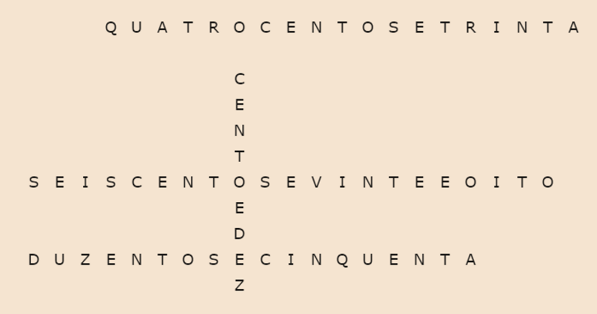
\includegraphics[width=\textwidth]{./media/image21.png}
\end{minipage}
\begin{minipage}{.3\textwidth}
\coment{Os números que podem compor o número 280 em sete parcelas
são: 10, 20, 30, 40, 50, 60 e 70. Esta atividade pode ser feita em
conjunto com a aula de ciências. Auxilie os alunos, pois a atividade
pode exigir um pouco mais deles.}
\end{minipage}\bigskip

Pinte as sete parcelas dos números que compõem o número central na ordem
crescente, conforme a ordem das cores do arco-íris.

\begin{figure}[htpb!]
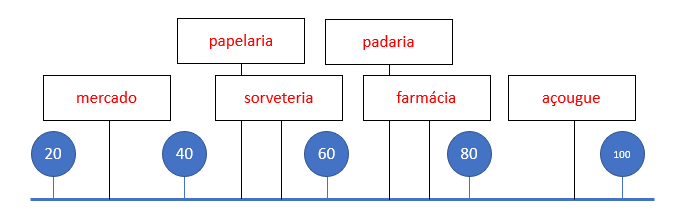
\includegraphics[width=\textwidth]{./media/image22.png}
\end{figure}

\pagebreak

\num{6} Jogar dardos é muito divertido. Considerando uma rodada com três arremessos no alvo representado, qual a pontuação máxima em um jogo?

\begin{figure}[htpb!]
\centering

\includegraphics[width=.4\textwidth]{./media/image23.png}
\end{figure}

\coment{Como o alvo identifica a pontuação máxima como 80, logo,
em uma rodada de três lançamentos, a pontuação máxima será 80 + 80 + 80 =
240 pontos.}

\num{7} Ainda pensando nos jogos de dardos, analise a explicação da figura a seguir.

\begin{figure}[htpb!]
\centering
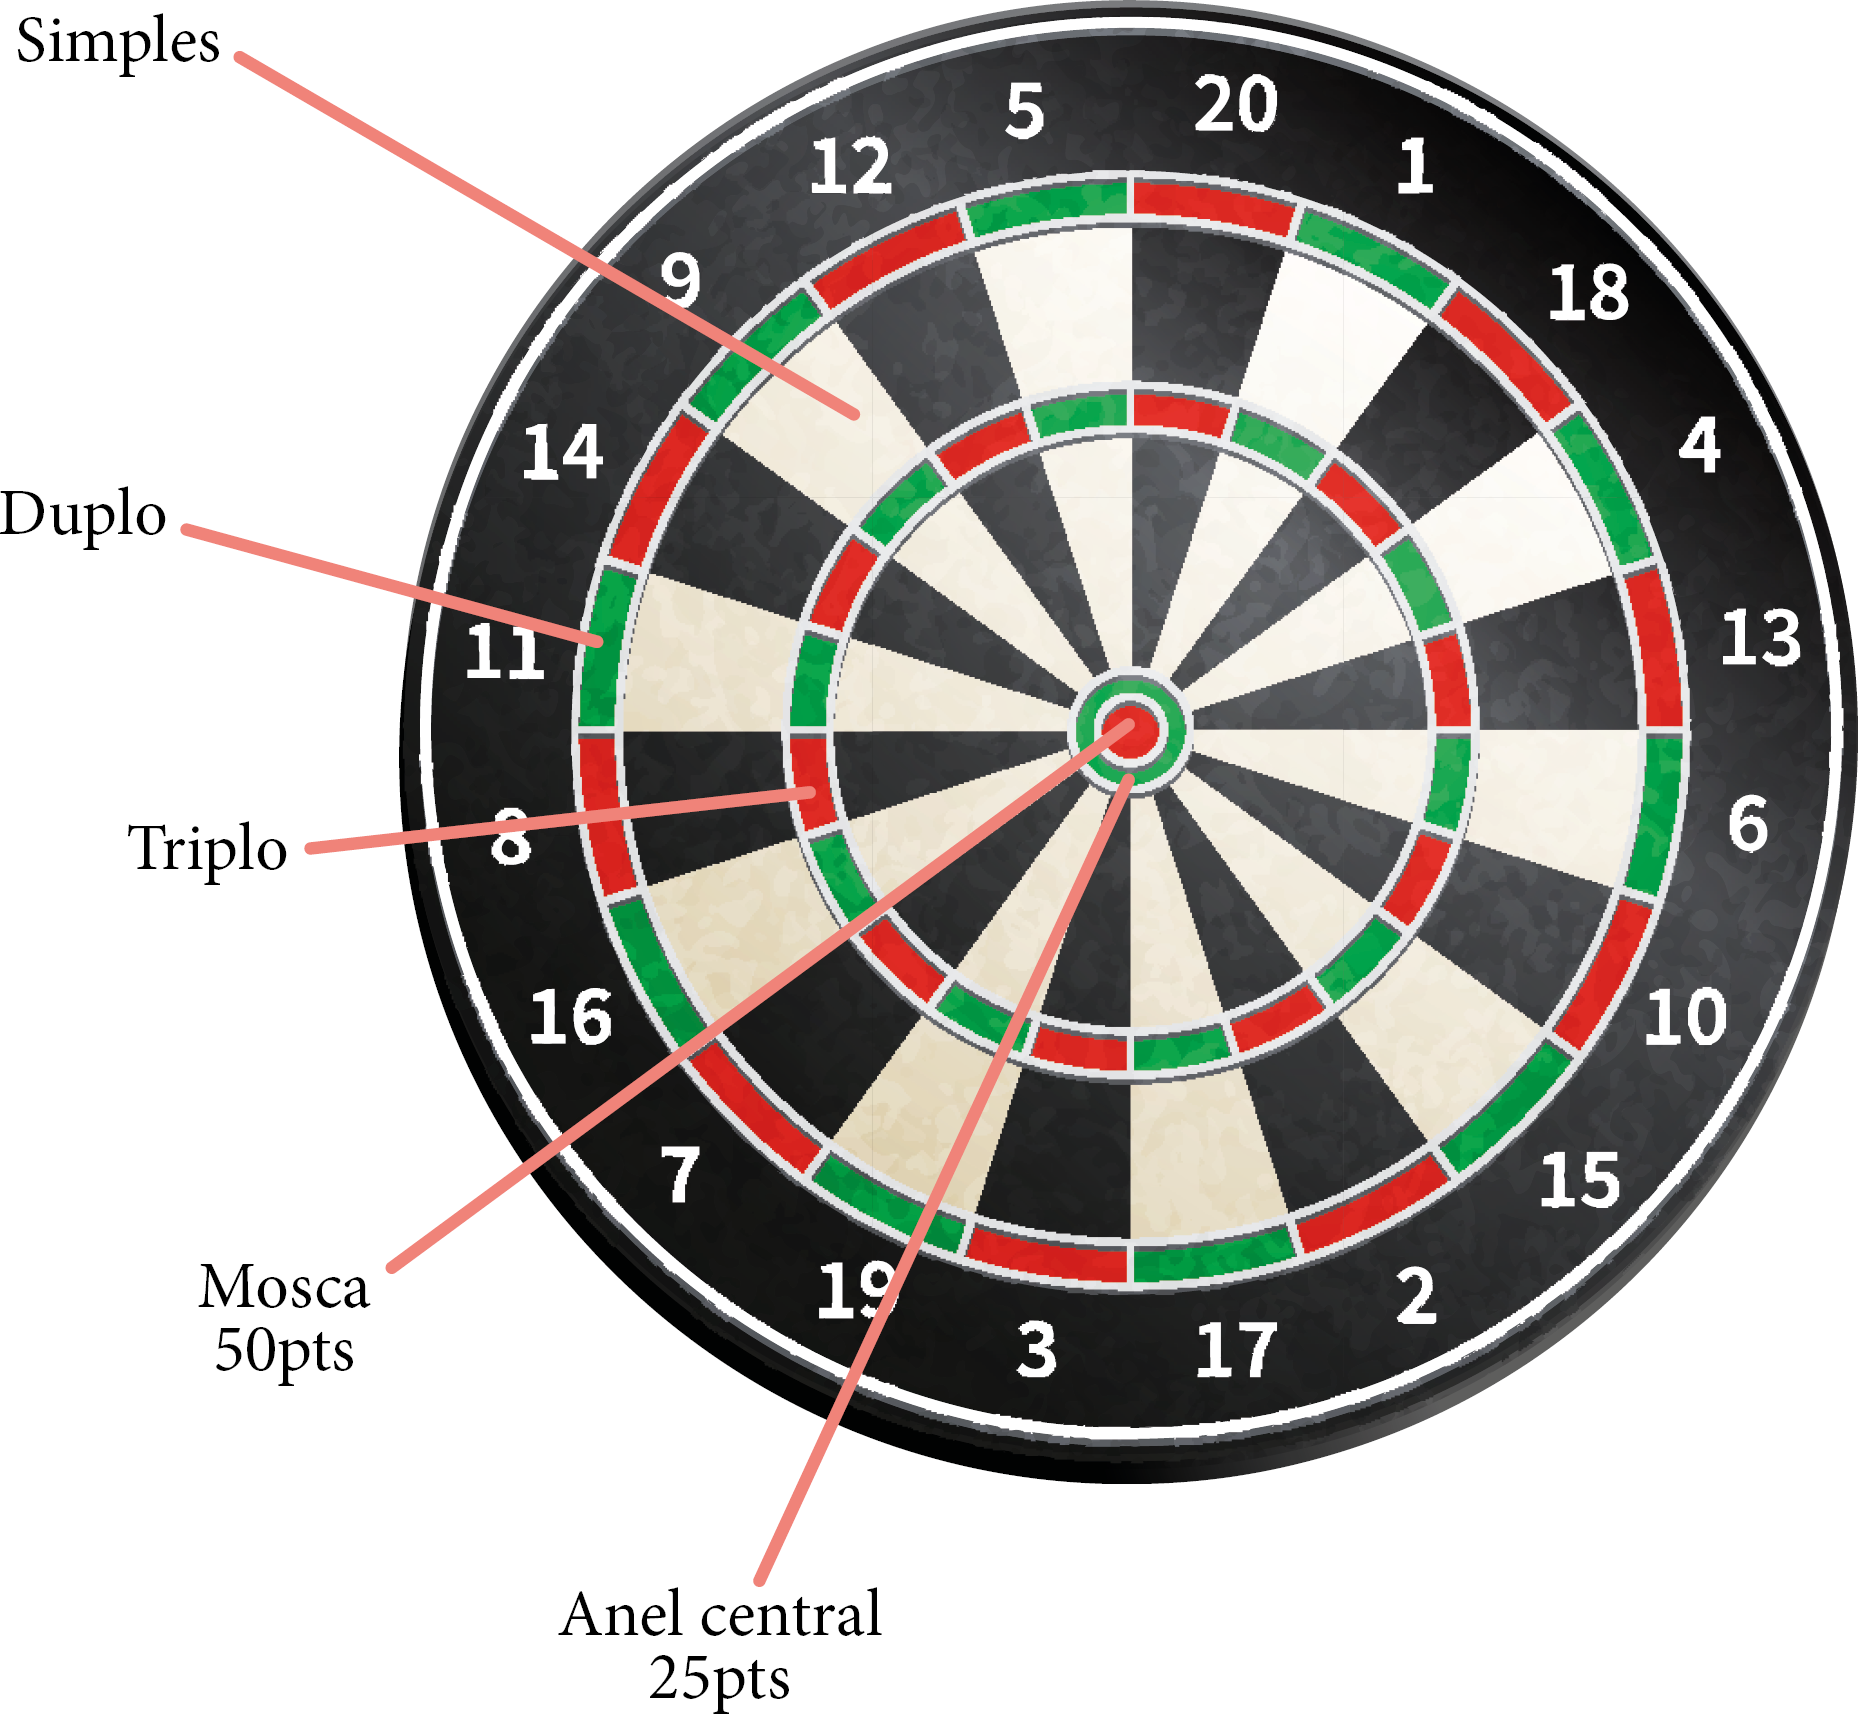
\includegraphics[width=.6\textwidth]{./media/image24.png}
\end{figure}

%\coment{Professor, é importante que você explique a pontuação dessa roleta. Não é difícil de entender, porém, os alunos podem ter dificuldade de interpretar a figura. Explique que, quando o dardo acerta as faixas finas marcadas em vermelho e verde, há pontuações extras: pontos duplicados no caso do verde e triplicados no caso do vermelho.}

\pagebreak
Calcule a pontuação das jogadas a seguir, onde os ``x'' azuis mostram onde o dardo acertou o alvo.

%https://br.freepik.com/vetores-premium/alvo-de-dardos-classico\_25927311.htm\#page=2\&query=dardos\&position=43\&from\_view=search\&track=sph

\begin{figure}[htpb!]
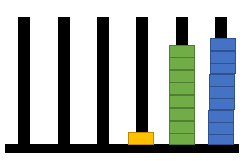
\includegraphics[width=.7\textwidth]{./media/image25.png}
\end{figure}

\pagebreak

\num{8} Marque, com três x, uma forma de fazer 100 pontos, utilizando 3 dardos no alvo a seguir.

\begin{figure}[htpb!]
\centering
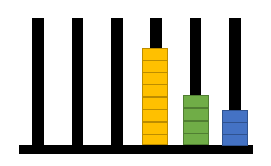
\includegraphics[width=.5\textwidth]{./media/image26.png}
\end{figure}

\coment{Temos várias combinações possíveis. Uma sugestão seria um
dardo no meio (50), outro dardo no duplo 20 e outro no simples 10.}

\num{9} Encontre no caça-palavras 4 números que, juntos, formam o número 570.

\begin{minipage}{.7\textwidth}
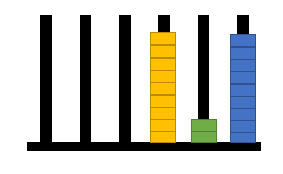
\includegraphics[width=\textwidth]{./media/image27.png}
\end{minipage}
\begin{minipage}{.3\textwidth}

\coment{Os números são duzentos, trezentos, quarenta e trinta. Ainda que os
alunos não saibam quais são os números, não existem outros no caça
palavras que não seja pertencente as parcelas do número 570. Portanto,
deixe que eles procurem os números, e, depois peça a eles que confiram a
adição.}
\end{minipage}

\pagebreak
\num{10}

Em um jogo de virar figurinhas, João apostou suas 24 figurinhas e Marcelo apostou suas 29. Na hora da disputa, João virou 15 figuras e Marcelo virou o resto. Responda o que se pede:

\begin{escolha}
\item Com quantas figurinhas Marcelo ficou?

\reduline{Primeiro, adicionamos as figurinhas de João e Marcelo: 24 + 29 = 53.
Depois retiramos as figuras que João virou do total: 53 - 15 = 38.\hfill}
\linhas{3}

\item Quantas figurinhas João perdeu?

\reduline{Retiramos as figuras que João tirou da quantidade que tinha antes da
disputa: 24 -- 15 = 9\hfill}
\linhas{2}

\item Quantas figuras Marcelo ganhou?

\reduline{Retiramos as figuras que Marcelo tinha antes da disputa do total que ganhou: 38 -- 29 = 9. O aluno poderia deduzir que, como o total de figurinhas era a soma das
figurinhas dos dois, antes da disputa, o que João perdeu é exatamente o
mesmo valor que Marcelo ganhou.\hfill}
\linhas{2}
\end{escolha}

% \num{11} Carlinhos tem uma coleção de 56 chaveiros. Ele guarda todos esses
% chaveiros em uma caixa de papelão e em um pote de plástico. Eles estão
% divididos por temas. Os da caixa de papelão são de times de futebol e os
% do pote de plástico são de marcas de carros. Carlinhos resolveu colocar
% todos no pote de plástico; logo, retirou os 35 chaveiros que estavam na
% caixa de papelão e os colocou no pote. Quantos chaveiros de marcas de
% carro Carlinhos tem?

% \reduline{Precisamos retirar a quantidade de chaveiros de times de futebol do
% total de chaveiros: 56 -- 35 = 21.\hfill}

\pagebreak
\colorsec{Treino}

\num{1} Lucas tem a incrível coleção de 236 \emph{cards} de diversos desenhos
animados. Seu amigo, Leonardo, tem uma coleção um pouco menor, com 132
\emph{cards}. Quantos \emph{cards} os dois têm juntos?

\begin{escolha}
\item 104

\item 366

\item 368

\item 398
\end{escolha}

\num{2} Indique a alternativa que contém uma composição do número 452.

\begin{escolha}
\item 150 + 129 + 173

\item 150 + 139 + 173

\item 150 + 143 + 179

\item 170 + 129 + 183
\end{escolha}


\num{3} A região Sul do Brasil tem apenas 3 estados. O Paraná, com 399
municípios; Santa Catarina, com 295 municípios; o Rio Grande do Sul, com
497 municípios. Quantos municípios a região Sul tem no total?

\begin{escolha}
\item 694

\item 792

\item 896

\item 1191
\end{escolha}

\chapter{Módulo 3}
\markboth{Módulo 3}{}

%\coment{Neste módulo, vamos desenvolver as habilidades concernentes aos conceitos de massa, volume e comprimento. Desenvolver nos alunos a ideia da necessidade de criarmos padrões de comparação para que medidas sejam feitas com cada vez mais precisão. }

\vspace*{-1cm}

\colorsec{Habilidades do SAEB}

\begin{itemize}
\item Comparar comprimentos, capacidades ou massas ou ordenar imagens de
  objetos com base na comparação visual de seus comprimentos, capacidades ou massas.

\item Estimar/inferir medida de comprimento, capacidade ou massa de objetos,
  utilizando unidades de medida convencionais ou não, ou medir
  comprimento, capacidade ou massa de objetos.

\item Identificar a medida de comprimento, da capacidade ou da massa de
  objetos, dada a imagem de um instrumento de medida.

\item Reconhecer unidades de medida e/ou instrumentos utilizados para medir
  comprimento, tempo, massa ou capacidade.
\end{itemize}

\colorsec{Habilidades da BNCC}

\begin{itemize}
\item EF02MA16, EF02MA17.
\end{itemize}

\conteudo{
%\textless{} https://br.freepik.com/fotos-gratis/familia-deitada-na-grama\_1165875.htm\#query=v\%C3\%A1rios\%20p\%C3\%A9s\&position=12\&from\_view=search\&track=ais\textgreater{}

\begin{wrapfigure}{r}{.5\textwidth}
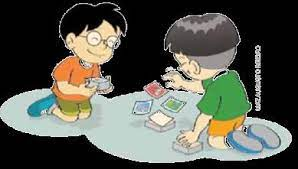
\includegraphics[width=.5\textwidth]{./media/image28.png}
\end{wrapfigure}

Você sabe qual o número do seu sapato? Ou melhor, você sabe qual número você calça? Já ouviu essa pergunta?
Ou, então, já ouviu algum familiar perguntando isso para sua mãe, pois
quer te dar um par de tênis de presente? Pois é! Calçados têm números para
representar os seus tamanhos. Mas como isso é medido? Todos temos
tamanhos padronizados de pés? É claro que não!
}

\conteudo{
Cada um de nós tem um
tamanho de pé. Mas, então, como a loja tem sapatos prontos, esperando
para serem vendidos para qualquer um? Existem vários padrões para numerar
um sapato. No Brasil, usamos o mesmo padrão usado na França. Quando
alguém usa um sapato 33, significa que o pé dessa pessoa tem até 21,6
centímetros. A cada 6,6 milímetros, temos um ponto. Vamos lá! Você já
tentou medir seu pé alguma vez? Pegue uma folha e trace o contorno do
seu pé com um lápis ou uma canetinha. Depois, meça do calcanhar até a
ponta do dedão em linha reta. Compartilhe as medidas entre os colegas.
Quem será que tem o maior pé? 

%\textless{} https://www.adidas.com.br/tabela\_de\_tamanhos\_adidas.html\textgreater{}

\noindent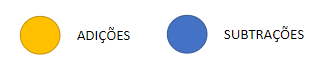
\includegraphics[width=\textwidth]{./media/image29.png}
}

\pagebreak
\colorsec{Atividades}

\num{1} Analise a figura e responda:

\begin{figure}[htpb!]
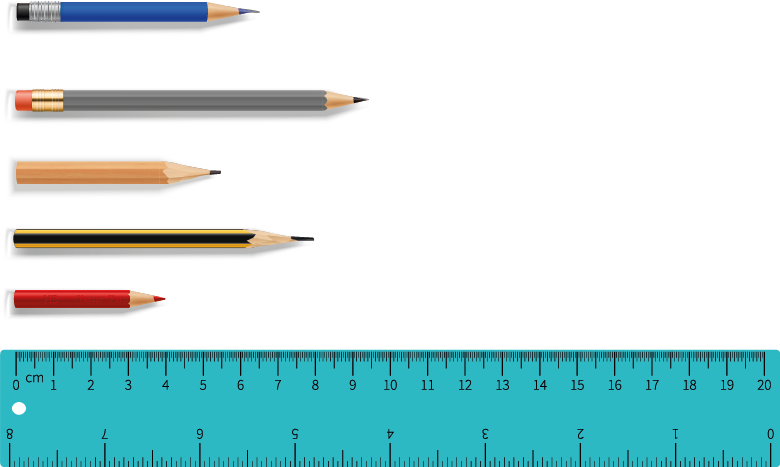
\includegraphics[width=.9\textwidth]{./media/image30.png}
\end{figure}

\begin{escolha}
\item  Qual cor de lápis tem aproximadamente 9 cm?

\reduline{O lápis de cor verde.\hfill}

\item  Qual cor de lápis tem aproximadamente 8 cm?

\reduline{O lápis de cor vermelha.\hfill}

\item  Qual cor de lápis tem aproximadamente 7 cm?

\reduline{O lápis de cor amarela.\hfill}

\item  O lápis azul é maior, menor ou igual a 7 cm?

\reduline{O lápis de cor azul é menor do que 7 cm.\hfill}

\item  O lápis rosa é maior, menor ou igual a 3 cm?

\reduline{O lápis de cor rosa é maior do que 3 cm.\hfill}
\end{escolha}

\pagebreak
\num{2} Analise a figura, leia o texto e responda ao que se pede.

%\textless{}https://br.freepik.com/vetores-gratis/fundo-de-edificio-de-escritorio-moderno\_2850420.htm\#page=2\&query=pr\%C3\%A9dios\&position=26\&from\_view=search\&track=sph\textgreater{}

\begin{figure}[htpb!]
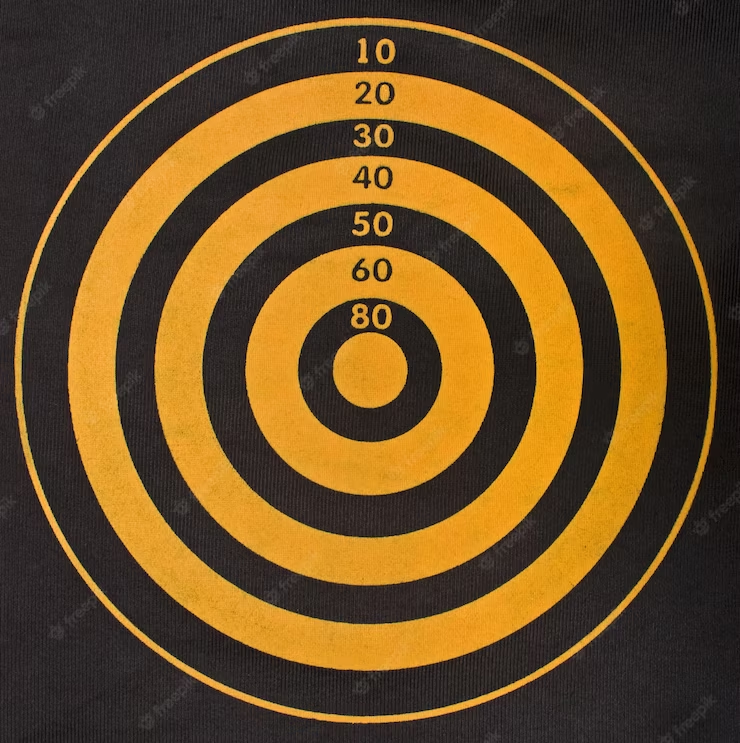
\includegraphics[width=\textwidth]{./media/image31.png}
\end{figure}

O prédio mais alto tem 50 metros de altura; o segundo prédio mais alto
tem 40 metros de altura; os dois prédios que parecem ser do mesmo
tamanho têm 30 metros de altura e o prédio roxo é o mais baixo entre
todos eles.

Qual é o tamanho aproximado do prédio mais baixo, na sua opinião?
Explique como chegou a essa conclusão.

\reduline{Espera-se que o aluno estime um valor próximo de 20
metros, caso perceba que os prédios vão diminuindo de 10 e 10 metros no
texto. Como eles têm que explicar como chegaram à conclusão, essa
atividade pode ser importante para desenvolver a habilidade de escrever
suas próprias ideias.\hfill}
\linhas{2}

\pagebreak
\num{3} Se a pessoa da figura ganhar 10 quilogramas, ficará com que massa?

%\textless{} https://br.freepik.com/vetores-gratis/ilustracao-de-perda-de-peso-de-mulher\_6086077.htm\#query=balan\%C3\%A7a\%20medindo\&position=5\&from\_view=search\&track=ais\textgreater{}

\begin{figure}[htpb!]
\centering
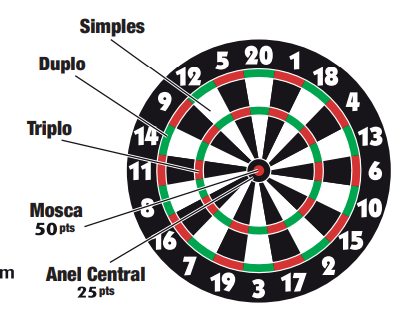
\includegraphics[width=.6\textwidth]{./media/image32.png}
\end{figure}

\reduline{81g, uma vez que a balança mede atualmente 70 kg.\hfill}

\num{4} O instrumento da foto, conhecido como gnômon, utiliza a sombra
provocada pelo Sol para marcar suas várias posições ao longo do dia. O
que este instrumento pode medir?

%\textless{}https://stock.adobe.com/br/images/id/296536857?get\_facets=1\&order=relevance\&safe\_search=1\&k=gnomon\&clickref=1101lwCPHVin\&mv=affiliate\&mv2=Freepik\&as\_camptype=\&as\_channel=affiliate\&as\_source=partnerize\&as\_campaign=Freepik\&as\_content=api\&as\_audience=srp\&sdid=6WTV6YJ5\textgreater{}

\begin{figure}[htpb!]
\centering
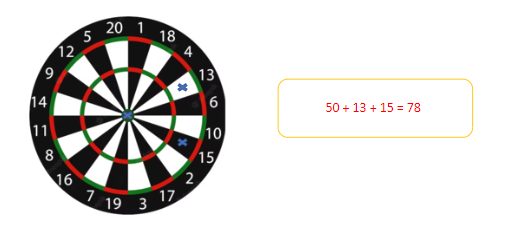
\includegraphics[width=.5\textwidth]{./media/image33.png}
\end{figure}

\reduline{Talvez o aluno não perceba que esse instrumento serve para
medir o tempo, uma vez que a ideia de posições pode confundi-lo, ou
induzi-lo a pensar que esse instrumento meça comprimento. É importante,
portanto, utilizar a atividade para mostrar aos alunos que duas
unidades podem ser combinadas para medir outra.\hfill}

\pagebreak
\num{5} A imagem a seguir mostra três objetos.

%\textless{}https://br.freepik.com/fotos-premium/podio-e-produto-de-podio-de-vidro-de-cena-de-palco-na-cena-de-podio-tres-produtos-de-renderizacao-em-3d\_33680968.htm\#query=copos\%20e\%20jarras\%20volume\&position=8\&from\_view=search\&track=ais Inserir as letras abaixo das figuras.\textgreater{}

\begin{figure}[htpb!]
\centering
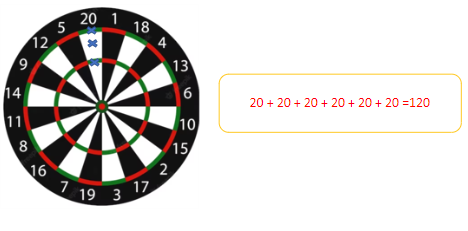
\includegraphics[width=.6\textwidth]{./media/image34.png}
\end{figure}

Compare os objetos e complete o quadro com os valores aproximados.

\begin{figure}[htpb!]

\includegraphics[width=\textwidth]{./media/image35.png}
\end{figure}

%\coment{É importante que o aluno perceba a proporção entre os objetos e consiga então inferir a capacidade do objeto do meio.}

\num{6} Complete os quadros corretamente, analisando as figuras dos tubos de
ensaio com exames de sangue. Estimando as capacidades ocupadas, indique
quais tubos têm as quantidades informadas no quadro.

%Inserir imagem https://br.freepik.com/fotos-vetores-gratis/sangue-tubo

\begin{figure}[htpb!]
\centering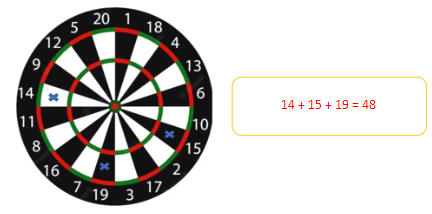
\includegraphics[width=.4\textwidth]{./media/image36.png}
\end{figure}

\begin{figure}[htpb!]
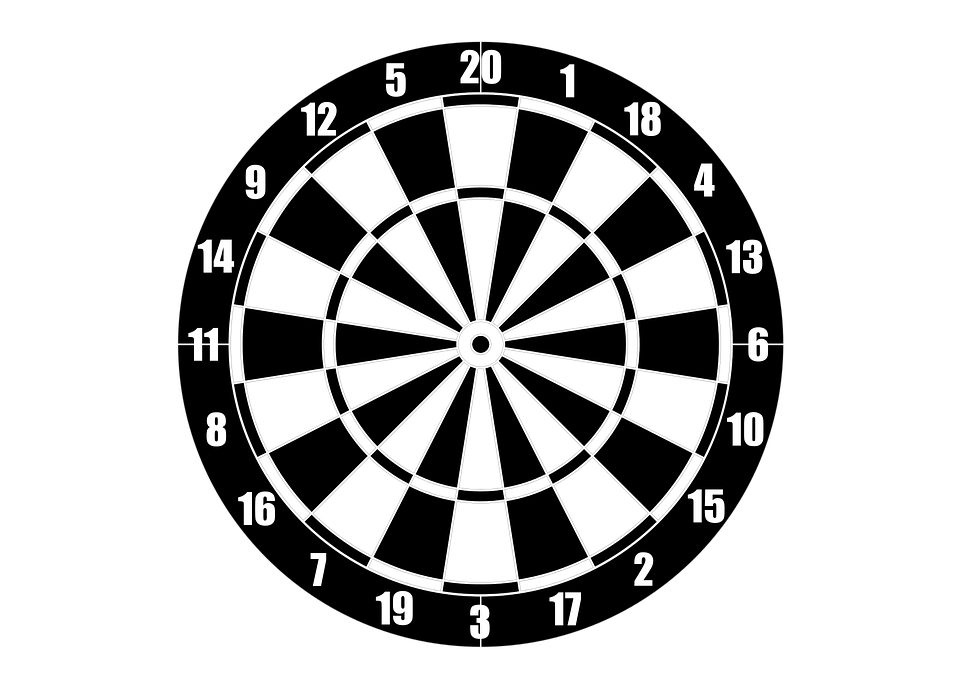
\includegraphics[width=\textwidth]{./media/image37.png}
\end{figure}

\pagebreak

\num{7} Indique pelo menos duas formas diferentes de medir algo, ou então dois
instrumentos que os meçam:

\begin{itemize}
\item Comprimento:

\reduline{uma régua e os próprios passos.\hfill}
\linhas{1}

\item Massa:

\reduline{Balança e comparar quantidades da mesma substância que tenha uma
indicação de massa na embalagem, por exemplo.\hfill}
\linhas{1}

\item Capacidade:

\reduline{copos ou seringas.\hfill}
\linhas{1}

\item Tempo:

\reduline{Relógio, cronômetro ou até a batida do próprio coração.\hfill}

\reduline{Aqui o importante é permitir que os alunos usem a criatividade e o raciocínio lógico.\hfill}
\end{itemize}

\num{8} Resolva a cruzadinha, descobrindo quais são os instrumentos de medida.

\begin{figure}[htpb!]
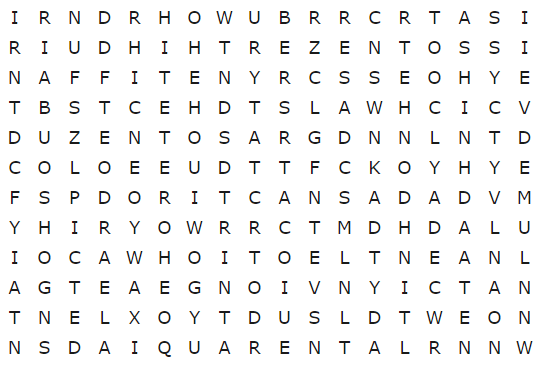
\includegraphics[width=\textwidth]{./media/image38.png}
\end{figure}

Horizontais:

1- Ele me diz se estou atrasado, ou se vou chegar a tempo.

3- Ela me diz se engordei ou emagreci, medindo minha massa.

4- Ela me diz o quanto cresci, além de medir o tamanho das coisas.

Verticais:

2- Ela guarda aquilo que mata minha sede, além de me ajudar a medir a
capacidade dos líquidos de ocupar espaço.

\num{9} Encontre unidades de medidas no caça-palavras.

\begin{figure}[htpb!]
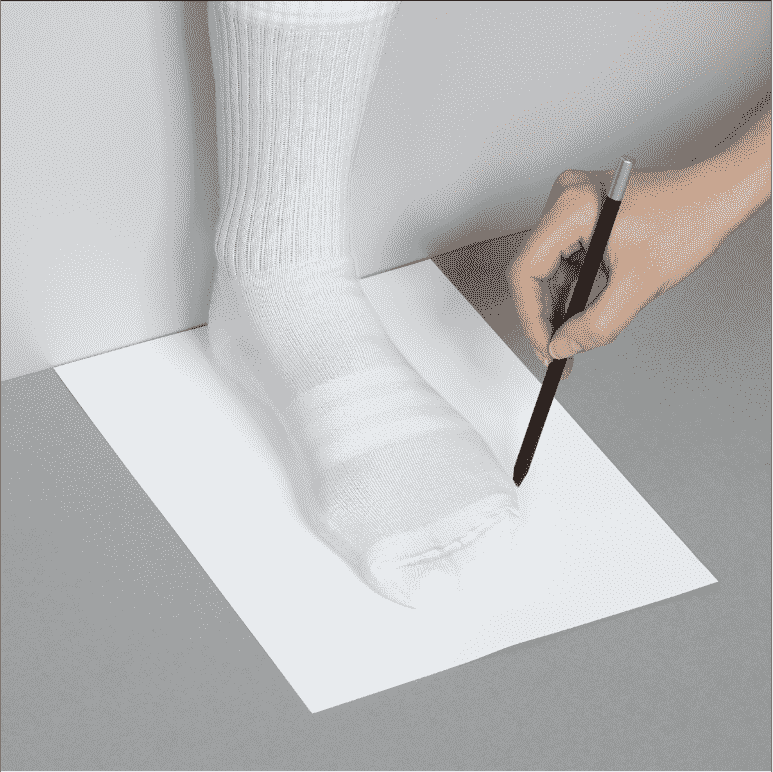
\includegraphics[width=\textwidth]{./media/image40.png}
\end{figure}

\coment{As palavras são: centímetro, mililitro, minutos, quilograma e segundos.}

\pagebreak
\num{10} Ligue a figura a sua massa em quilogramas, de forma correta.

\begin{figure}[htpb!]
\centering
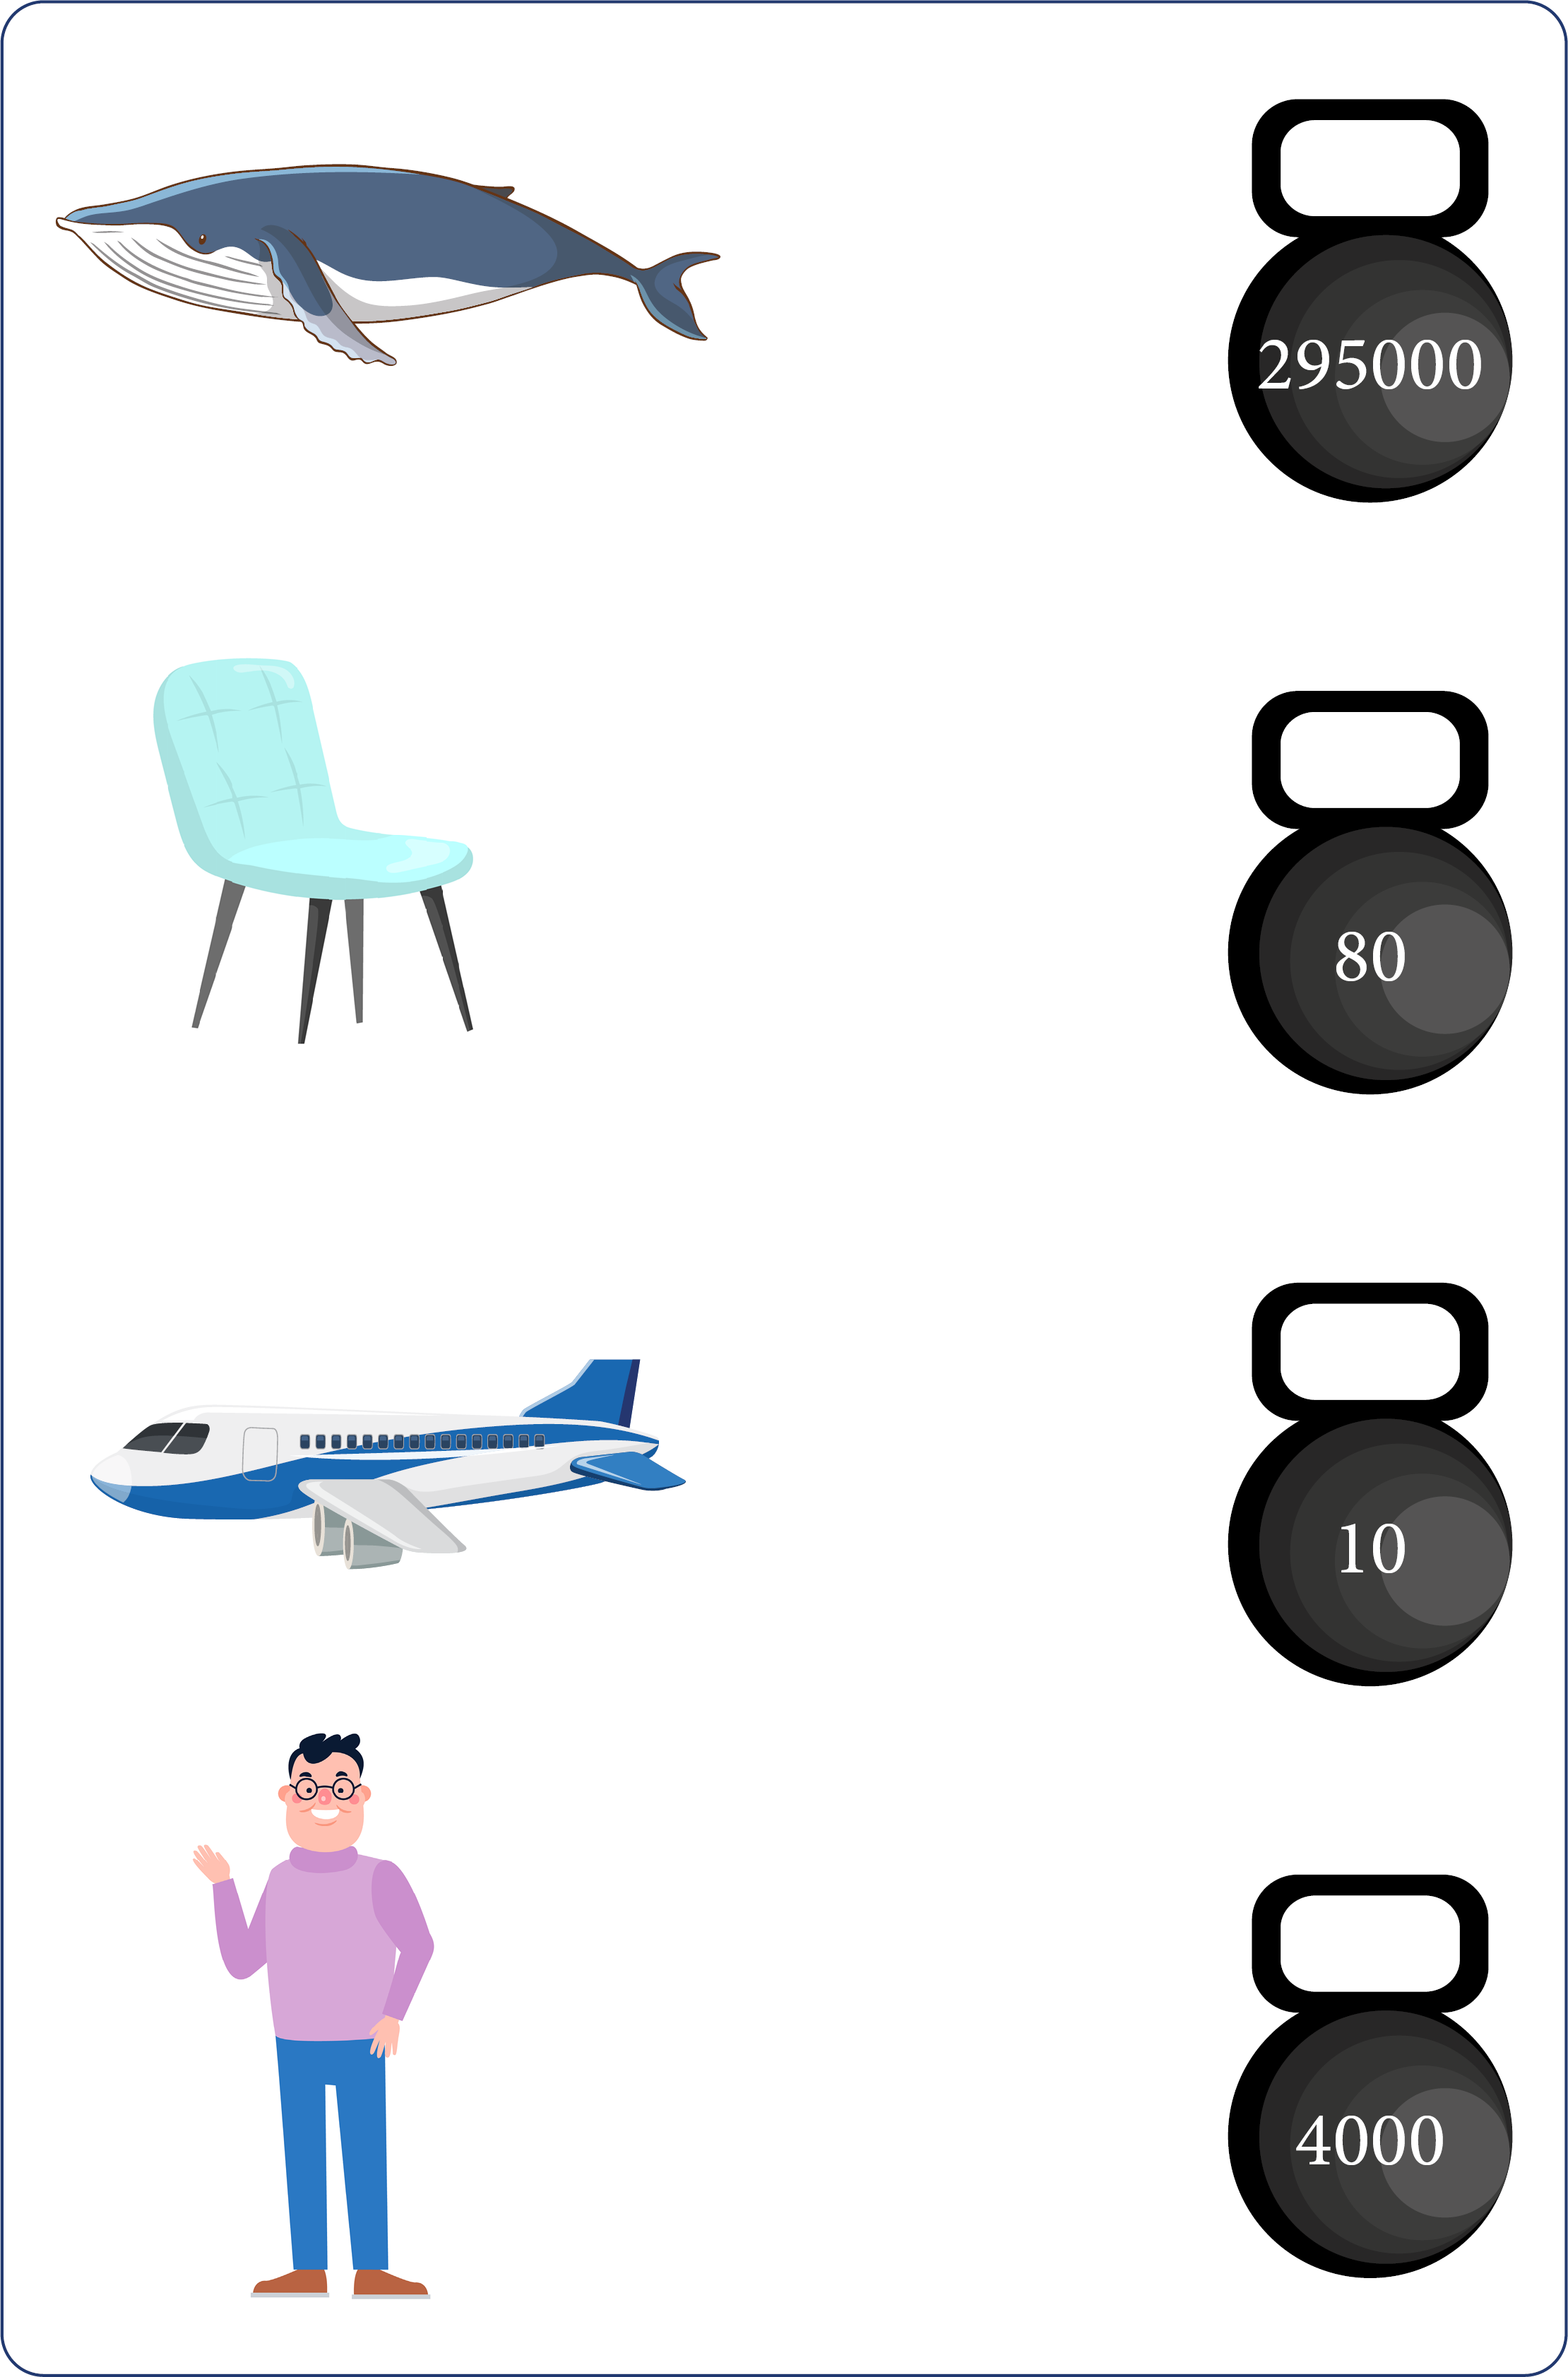
\includegraphics[width=.85\textwidth]{./media/image41.png}
\end{figure}

%\coment{As relações corretas são:
%Baleia -- 4.000
%Cadeira -- 10
%Avião -- 295.000
%Homem adulto -- 80}
\pagebreak
% \num{11} A figura mostra uma balança de ponteiros. Responda ao que se pede.

% \begin{figure}[htpb!]
% \centering
% 
\includegraphics[width=.7\textwidth]{./media/image42.png}
% \end{figure}

% \begin{escolha}
% \item  Qual é a capacidade máxima da balança, ou seja, qual é a maior massa que ela consegue medir?

% \reduline{1.000 gramas ou 1 quilograma.\hfill}

% \item  Quanto a balança está medindo na imagem?

% \reduline{250 gramas.\hfill}

% \pagebreak

% \item  Dá para medir a massa do pacote de arroz da figura a seguir nessa balança? Explique.

% %\textless{}https://br.freepik.com/vetores-premium/abra-o-icone-do-saco-de-arroz-pacote-de-tela-de-graos-asiaticos\_28762137.htm. Acrescentar a medida.\textgreater{}

% \begin{figure}[htpb!]
% \centering
% 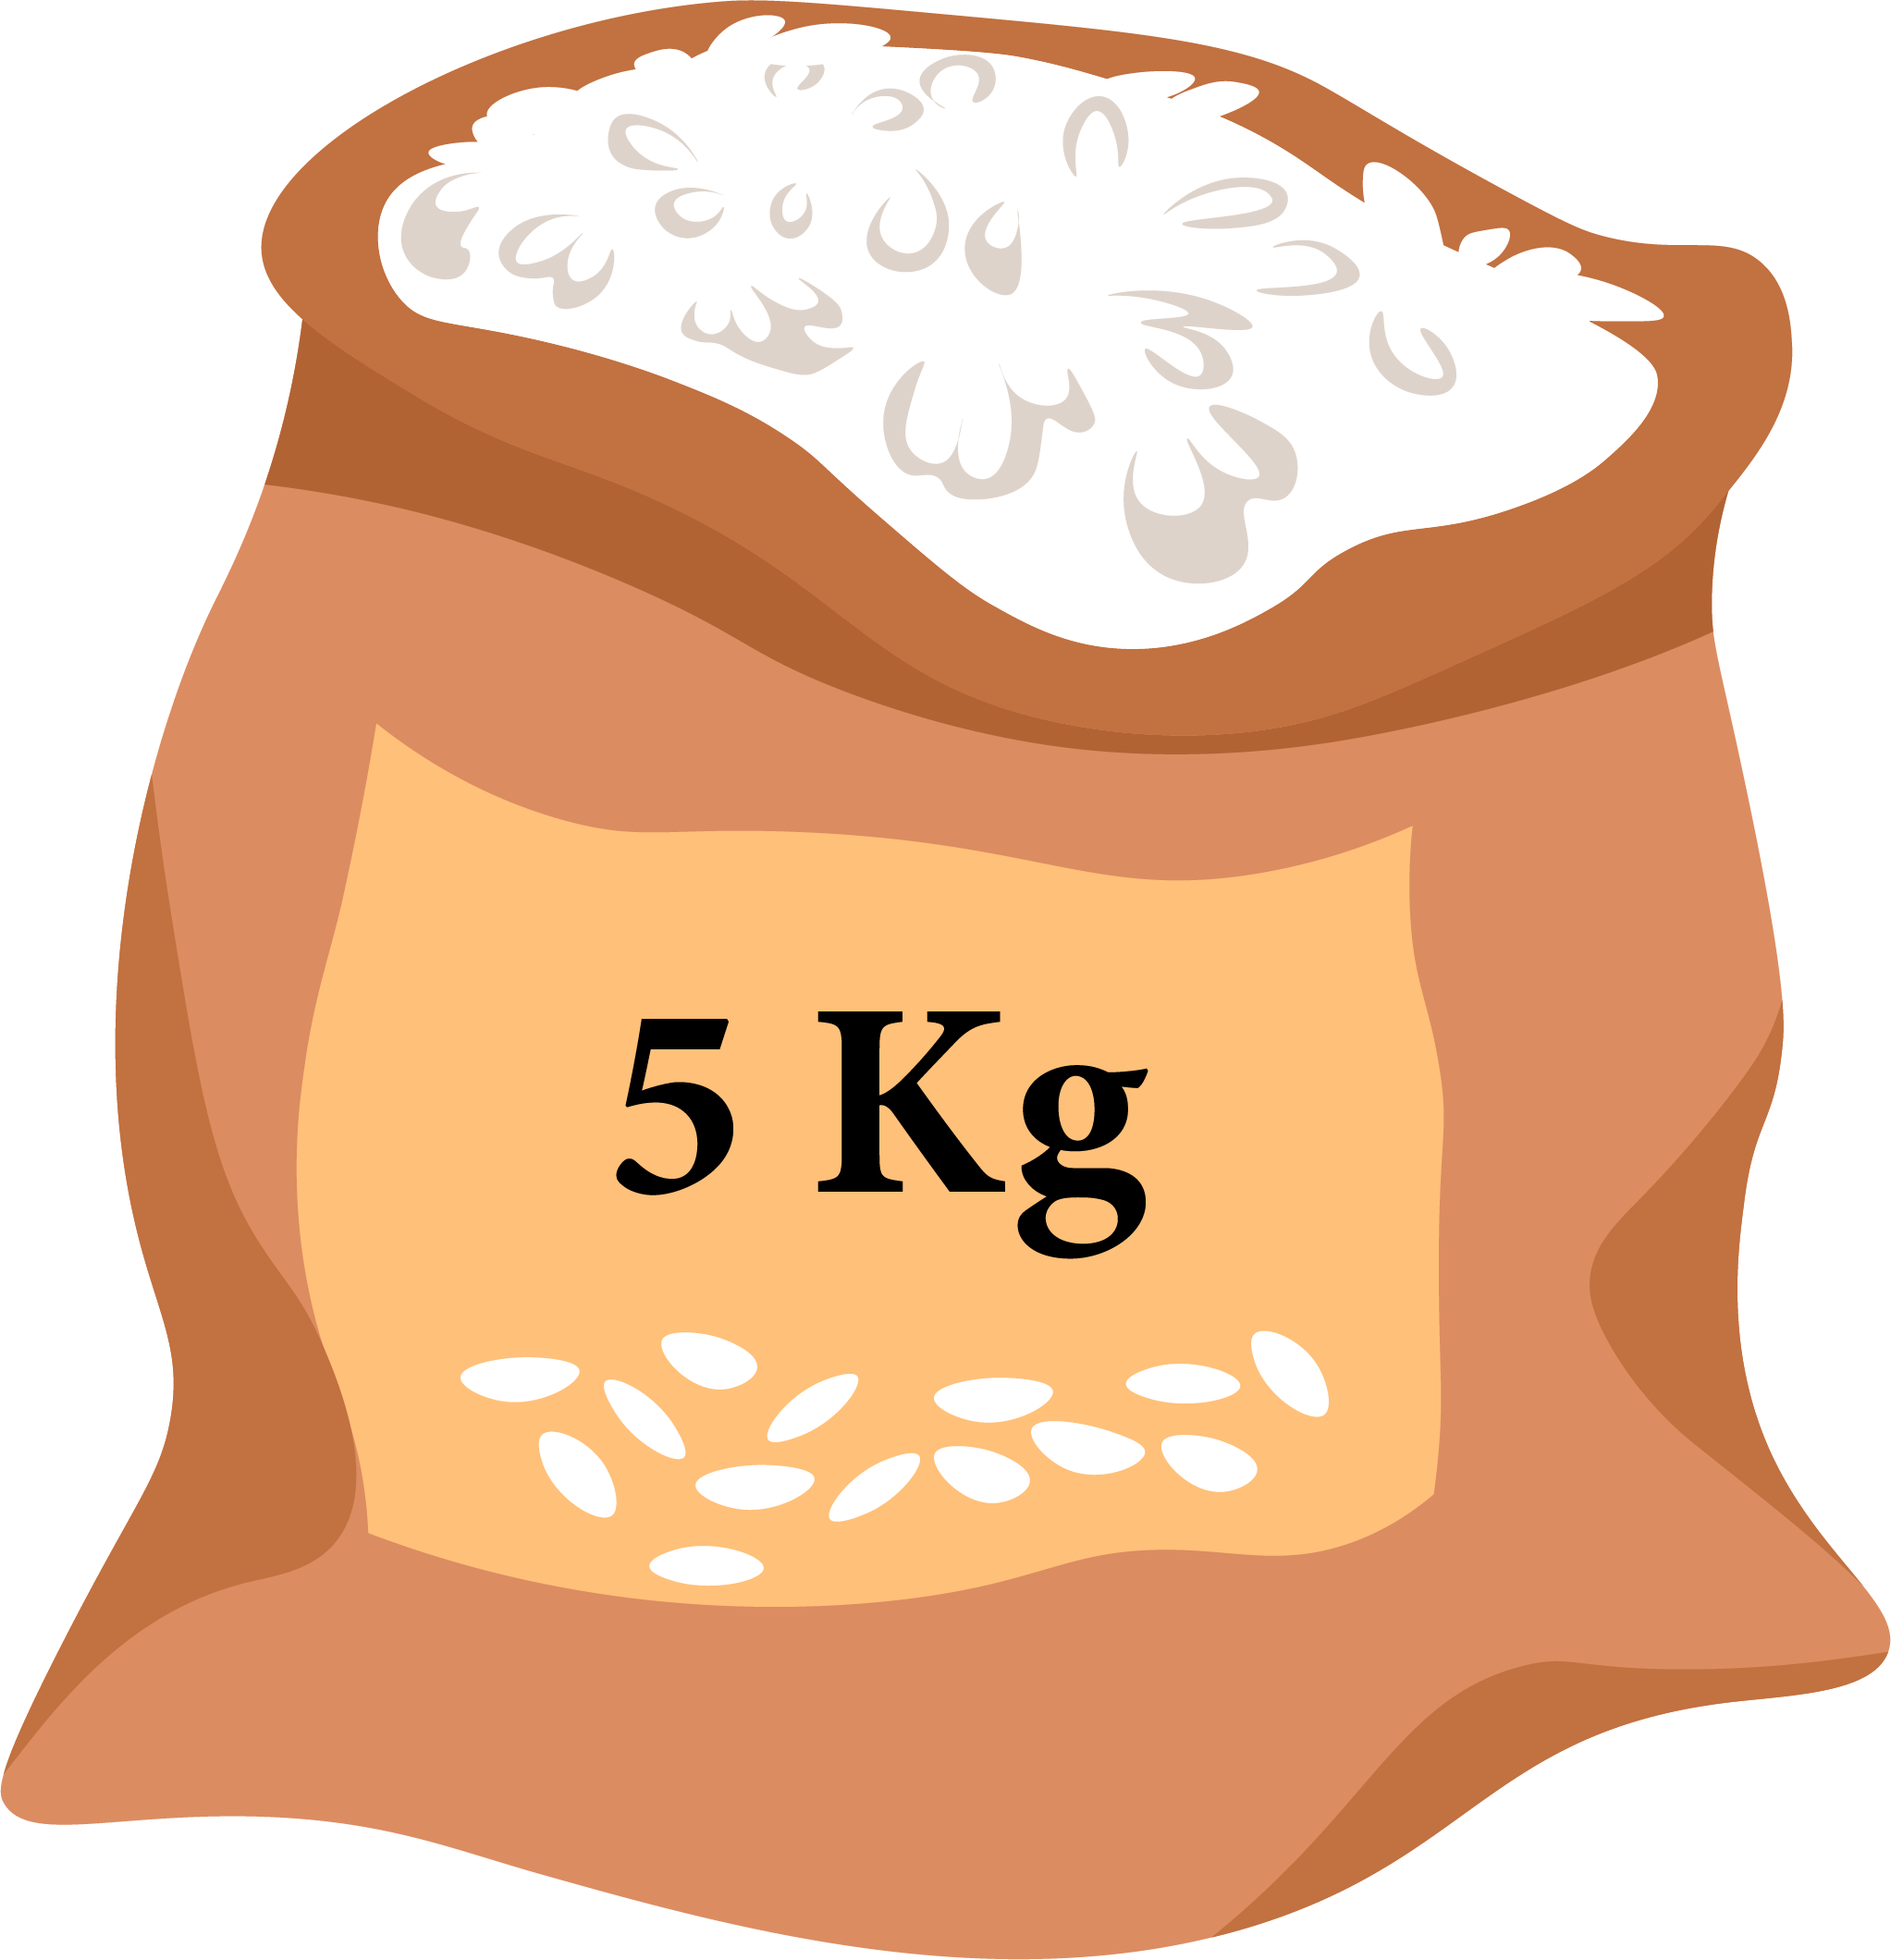
\includegraphics[width=.3\textwidth]{./media/image43.png}
% \end{figure}

% \reduline{Não dá, pois o saco de arroz tem 4 kg de massa, o que está além da capacidade da balança.\hfill}

% \item  Dá para medir a massa do pacote de café da figura a seguir nessa balança? Explique.

% %\textless{}https://br.freepik.com/vetores-gratis/colecao-dos-elementos-do-cafe\_1076091.htm\#query=caf\%C3\%A9\%20no\%20saco\&position=13\&from\_view=search\&track=ais. Acrescentar a medida. Substitua coffee bean por café.\textgreater{}

% \begin{figure}[htpb!]
% \centering
% 
\includegraphics[width=.2\textwidth]{./media/image44.png}
% \end{figure}

% \reduline{Dá para medir, pois a massa do pacote de café tem a metade da capacidade de medição da balança.\hfill}

% \item  Quanto mede cada risquinho da balança?

% \reduline{50 gramas.\hfill}
% \end{escolha}

\pagebreak
\colorsec{Treino}

\num{1} A menina da figura a seguir está usando os braços para medir:

%\textless{} https://br.freepik.com/vetores-premium/a-menina-mede-a-largura-usando-o-estiramento-da-mao\_24777556.htm\#query=medidas\&position=9\&from\_view=search\&track=sph\textgreater{}

\begin{figure}[htpb!]
\centering
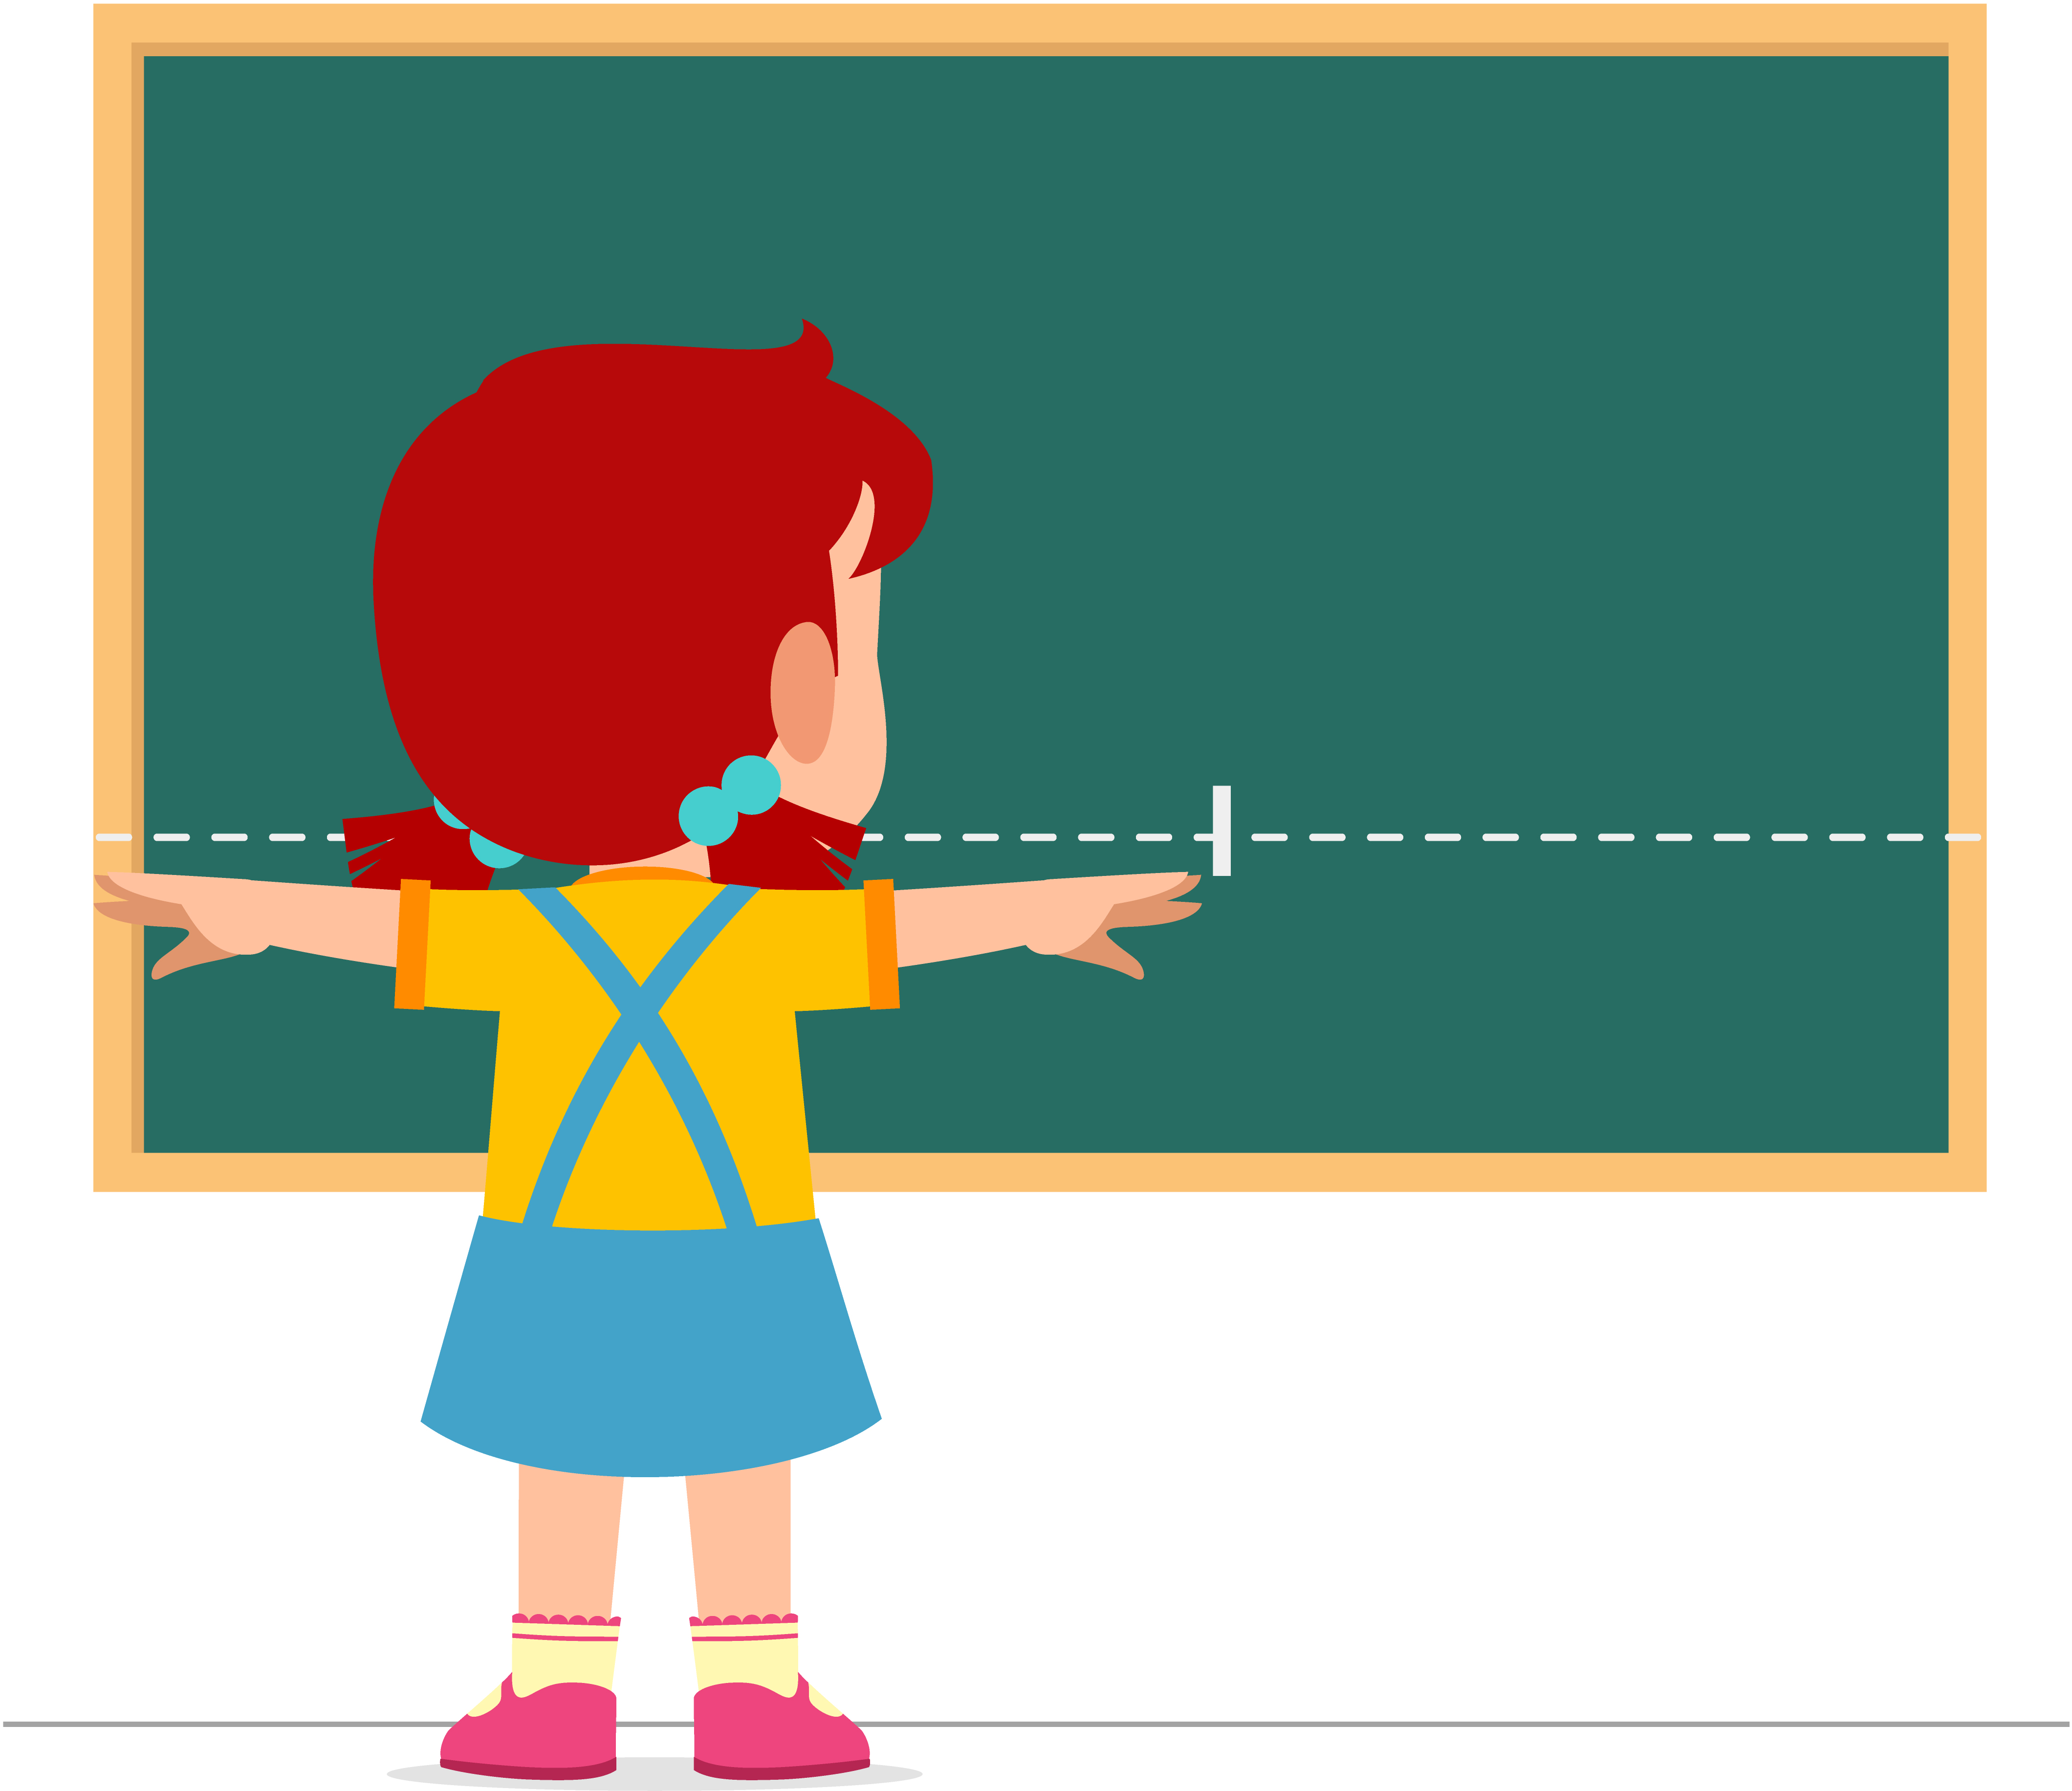
\includegraphics[width=.5\textwidth]{./media/image45.png}
\end{figure}

\begin{escolha}
\item Capacidade

\item Comprimento

\item Massa

\item Tempo
\end{escolha}

\num{2} A imagem mostra um tubo de ensaio com um líquido vermelho que será estudado.

%\textless{} https://br.freepik.com/fotos-gratis/closeup-tiro-de-um-conta-gotas-em-um-copo-com-um-liquido-vermelho-em-uma-parede-branca\_13006316.htm\#page=3\&query=tubo\%20de\%20ensaio\%20sangue\&position=8\&from\_view=search\&track=ais\textgreater{}

\begin{figure}[htpb!]
\centering
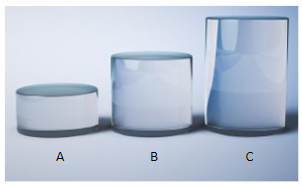
\includegraphics[width=.2\textwidth]{./media/image46.png}
\end{figure}

\pagebreak

Sabendo que dentro do conta-gotas, que é o tubinho menor dentro do tubo
maior, tem 5 mL do líquido vermelho, indique a alternativa que mostra a
quantidade total de líquido vermelho corretamente.

\begin{escolha}
\item Exatamente 10 mL.

\item Pouco menos de 20 mL.

\item Mais de 30 mL.

\item Exatamente 40 mL.
\end{escolha}

\num{3} A figura mostra o comprimento dos lados do parquinho da escola.
Estime o tamanho do lado A, do lado B, o comprimento total do contorno
do parquinho e, então, indique a resposta.

\begin{figure}[htpb!]
\centering
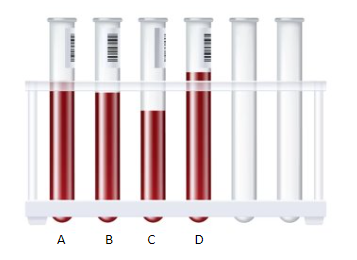
\includegraphics[width=.5\textwidth]{./media/image47.png}
\end{figure}

\begin{escolha}
\item a = 2, b = 5 e c = 7.

\item a = 5, b = 2 e C = 11.

\item a = 5, b = 2 e c = 18.

\item a = 2, b = 5 e c = 18.
\end{escolha}

\chapter{O juiz apita}
\markboth{Módulo 4}{}

%\coment{Neste módulo, vamos desenvolver nos alunos a habilidade de orientar-se no tempo, sabendo identificar o tempo presente, assim como prever dias e horários de eventos futuros. }
\vspace*{-1cm}

\colorsec{Habilidades do SAEB}

\begin{itemize}
\item Identificar sequência de acontecimentos relativos a um dia.

\item Identificar datas, dias da semana ou meses do ano em calendário ou
escrever uma data, apresentando o dia, o mês e o ano.

\item Determinar a data de início, a data de término ou a duração de um
acontecimento entre duas datas.

\item Determinar o horário de início, o horário de término ou a duração de
um acontecimento.
\end{itemize}

\colorsec{Habilidades da BNCC}

\begin{itemize}
\item EF02MA18, EF02MA19.
\end{itemize}

\conteudo{
Você já parou pra pensar quanto tempo demora um jogo de um esporte
qualquer? Às vezes vamos jogar bola e não nos damos conta do tempo que
passa. Simplesmente, jogamos até cansarmos, ou então até nossa mãe nos
chamar para entrar. Nos esportes profissionais, porém, não pode ser
assim. Cada modalidade tem o seu tempo determinado. Mas será que temos o
mesmo tempo para todas as modalidades? Será que todas são medidas pelo
tempo? Vamos analisar alguns esportes e compará-los. Veja o quadro na página ao lado. 
}

\pagebreak
\conteudo{
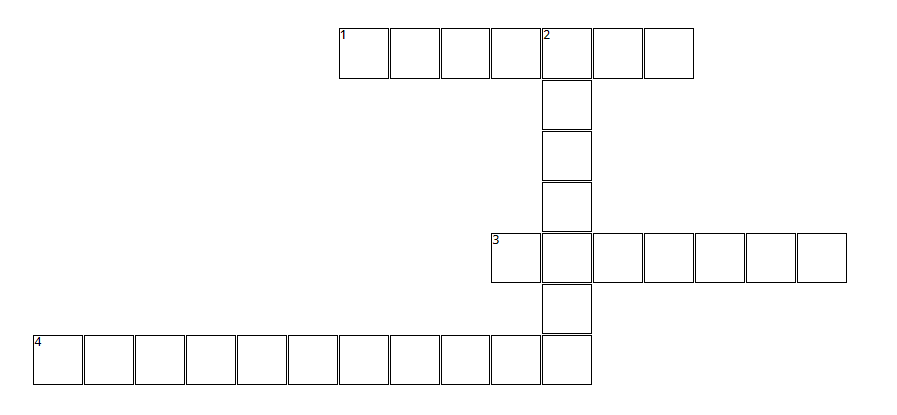
\includegraphics[width=\textwidth]{./media/image48.png}

O tempo de jogo de cada esporte é pensado de forma a não forçar os
atletas além de suas capacidades físicas. Também é levado em
consideração o espetáculo, afinal de contas todo esporte tem o seu
público, que acompanha os jogos, torce e tem seus jogadores favoritos.
}

\colorsec{Atividades}

\num{1} Complete o quadro.

\begin{figure}[htpb!]
\centering
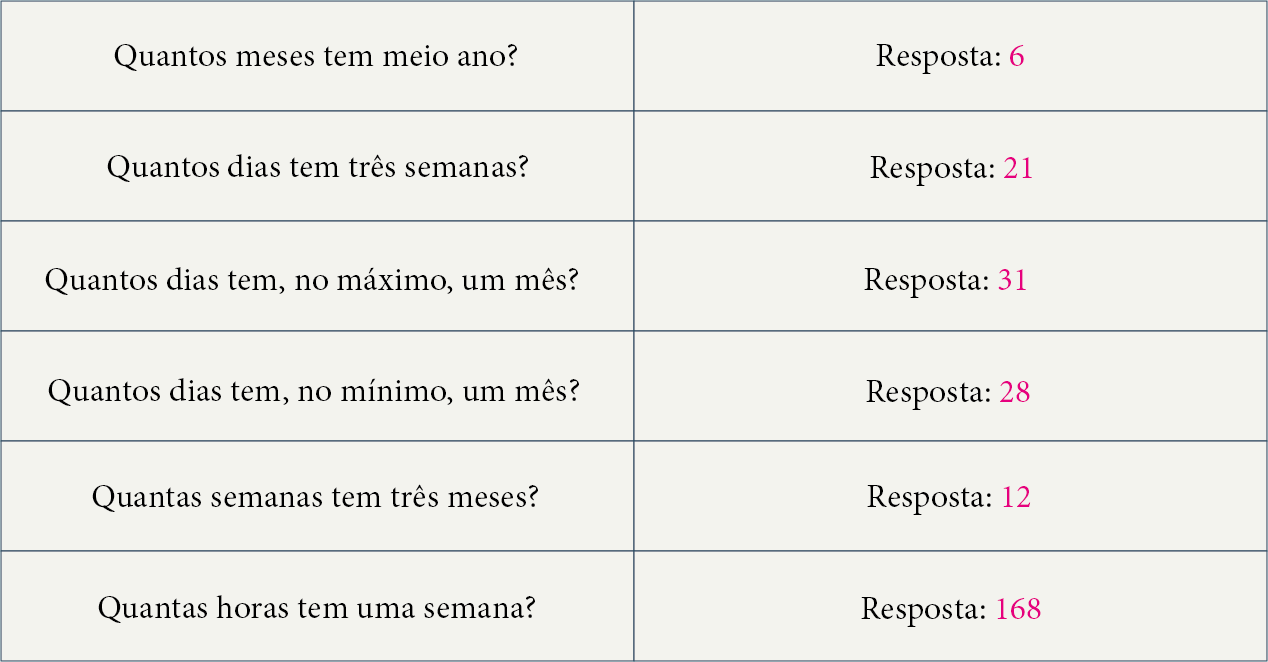
\includegraphics[width=.9\textwidth]{./media/image50.png}
\end{figure}

\pagebreak
\num{2} Organize as tarefas ou atividades na linha do tempo de um dia, conforme
sua realidade. Preencha os números das atividades na sequência em que acontecem com você. Insira atividades que não estejam listadas nos números que aparecem em branco.

\begin{figure}[htpb!]
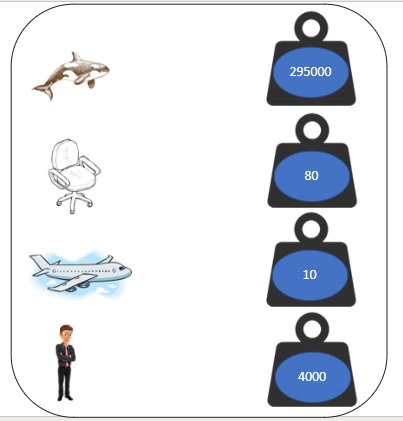
\includegraphics[width=\textwidth]{./media/image51.png}
\end{figure}

\coment{A atividade não tem uma resposta determinada, pois dependerá do cotidiano do aluno. O importante é que cada um consiga organizar, na linha do tempo, sua própria rotina, de forma lógica.}

\pagebreak
\num{3} Analise o calendário de 2023 e indique o dia da semana dos eventos pedidos.

%\textless{} https://7calendar.com/pt/calendar/p-1/ . É importante que o calendário tome uma folha. \textgreater{}

\begin{figure}[htpb!]
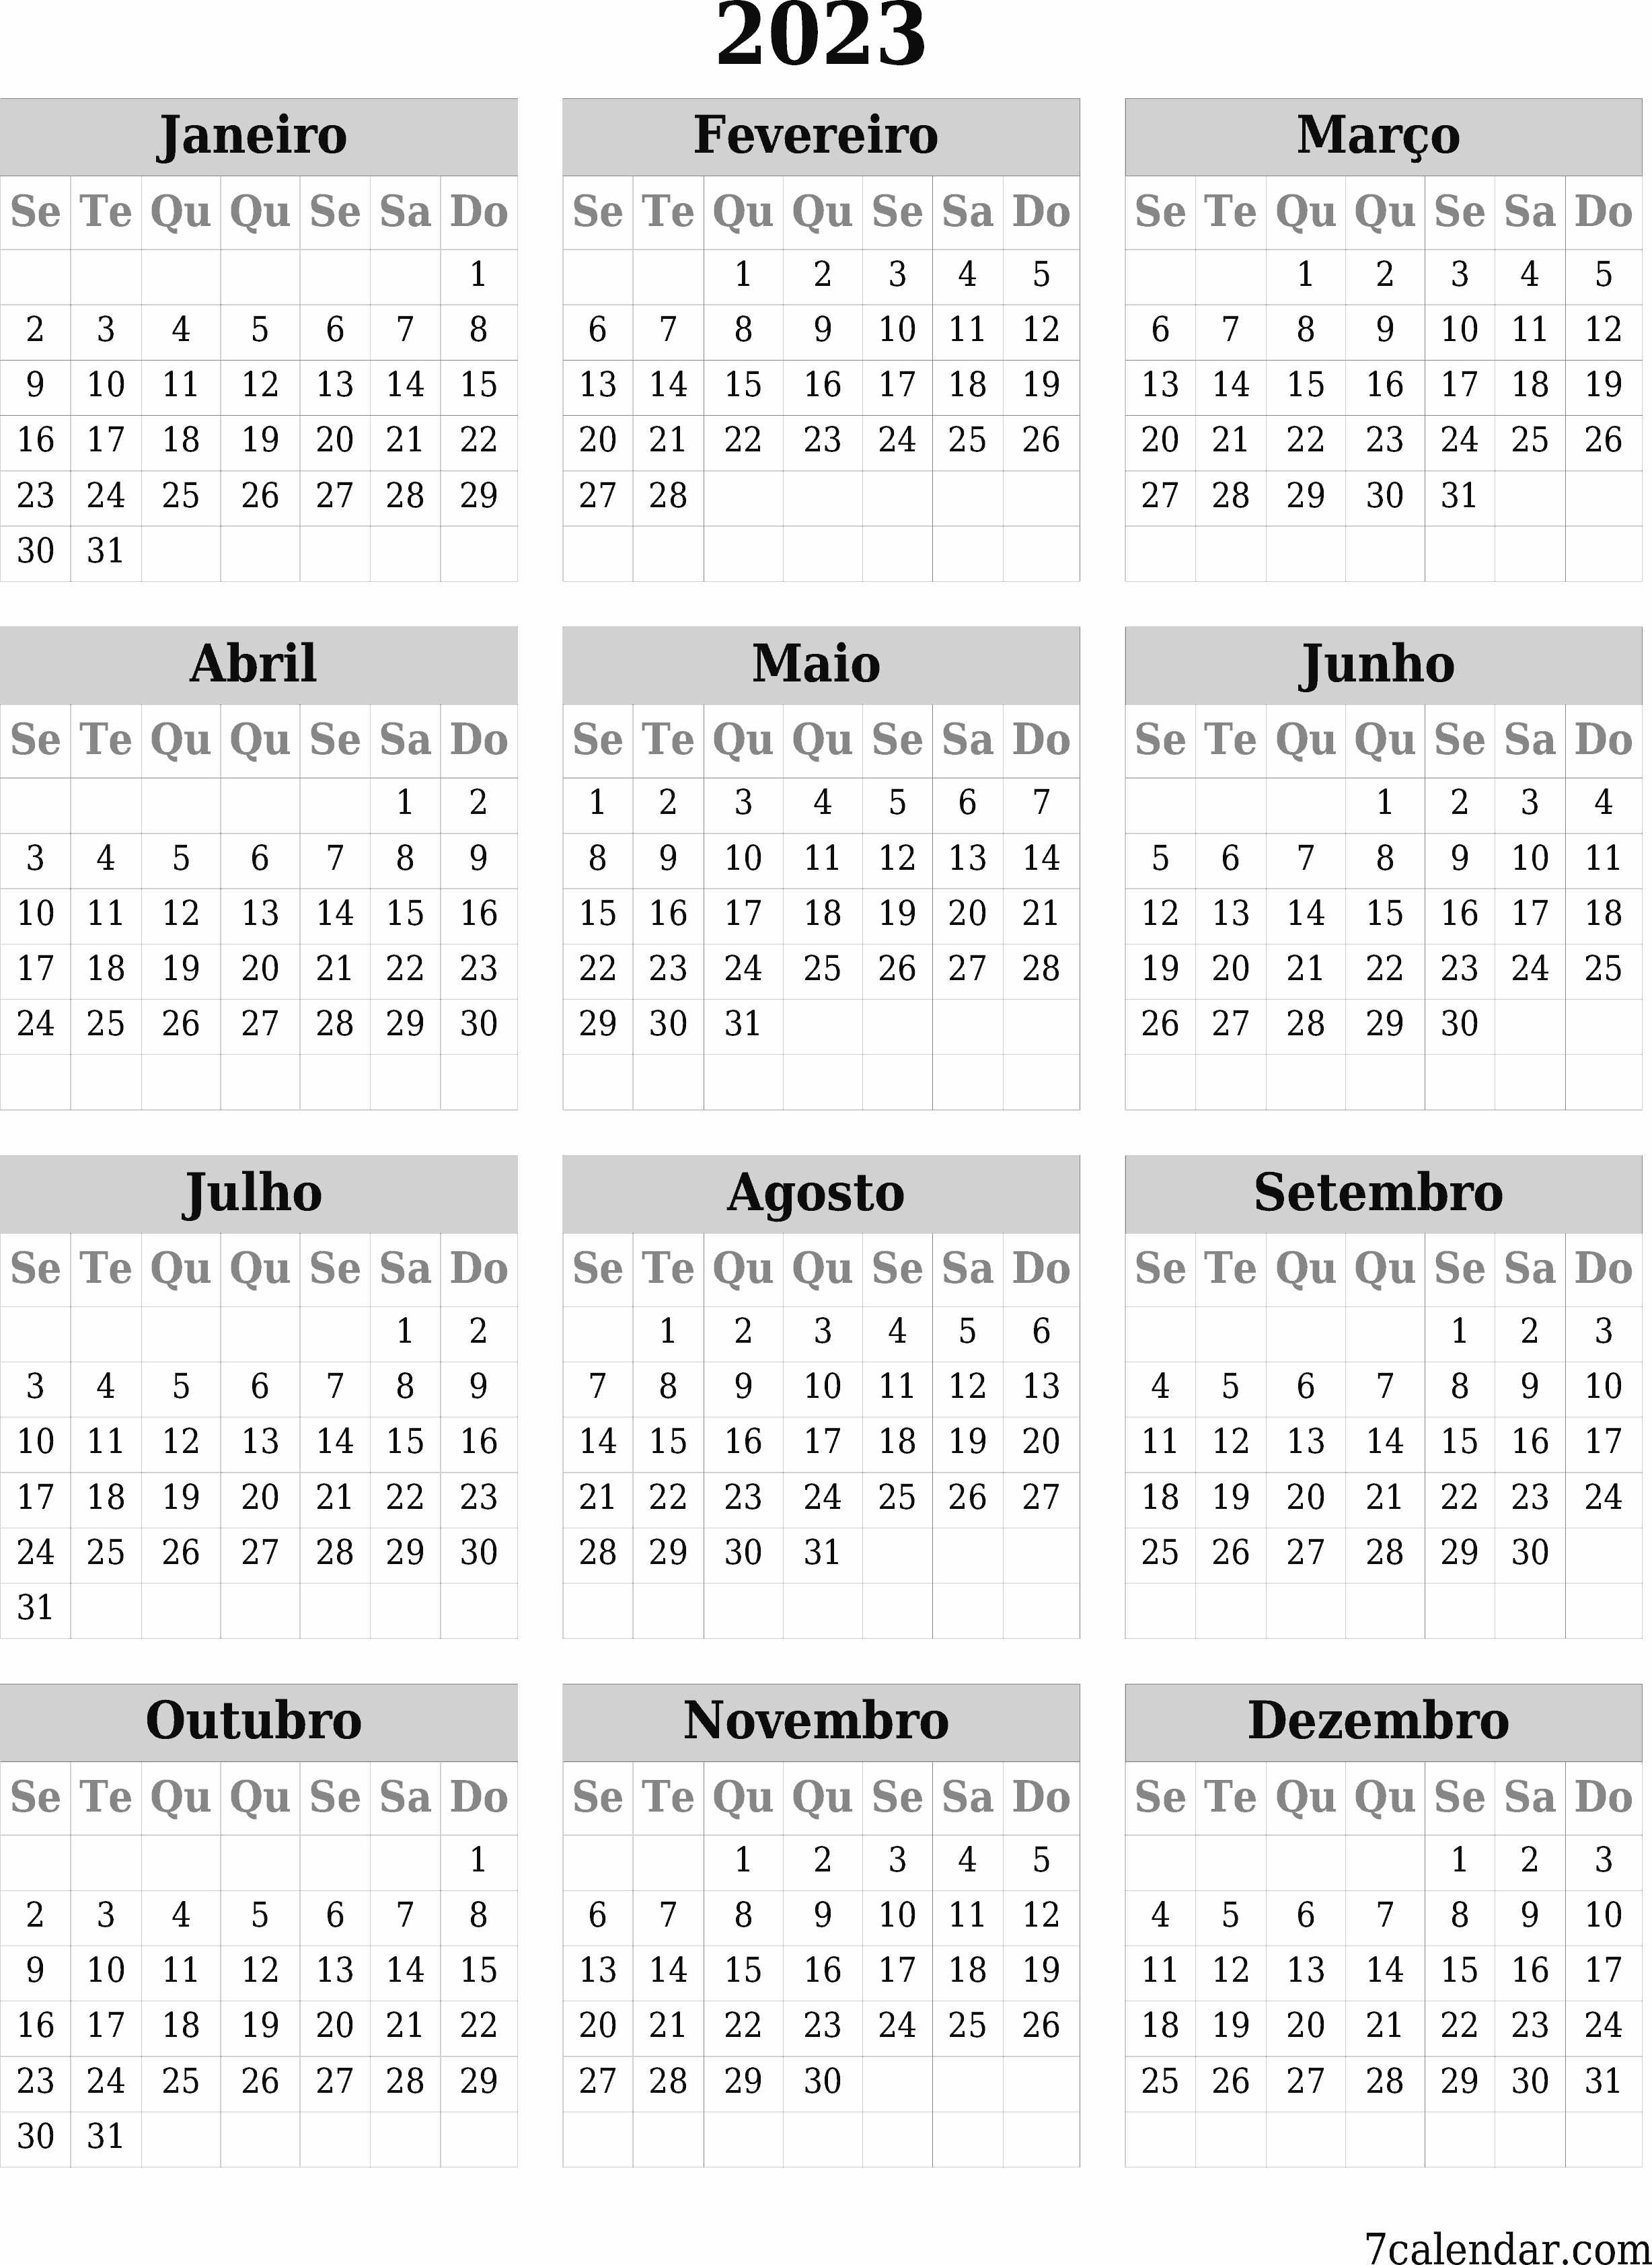
\includegraphics[width=\textwidth]{./media/image52.png}
\end{figure}

\begin{escolha}
\item  Páscoa - 9 de abril.

\reduline{Domingo.\hfill}

\item  Dia das Mães - 14 de maio.

\reduline{Domingo.\hfill}

\item  Independência do Brasil - 7 de setembro.

\reduline{Quinta-feira.\hfill}

\item  Dia das Crianças - 12 de outubro.

\reduline{Quinta-feira.\hfill}

\item  Proclamação da República - 15 de novembro.

\reduline{Quarta-feira.\hfill}
\end{escolha}

\num{4} Joaquina foi ao dentista no dia 06 de janeiro de 2023 e fez uma
obturação. O dentista pediu para ela voltar 15 dias depois da primeira
consulta. Sabendo disso, complete o quadro. (Utilize o calendário
da atividade anterior.)

\begin{figure}[htpb!]
\includegraphics[width=\textwidth]{./media/image53.png}
\end{figure}

\pagebreak
\num{5} Todo dia 1° de maio, de todos os anos, comemoramos o Dia do Trabalhador,
assim como todo dia 20 de julho, também de todos os anos, comemoramos o
Dia Internacional da Amizade. Quantos dias se passam entre essas duas
comemorações, sem contar as datas em si?

\reduline{Permita que os alunos escolham as suas próprias
estratégias para resolverem esse problema. Eles podem simplesmente
contar os dias no calendário, ou tentar fazer isso por meio dos
cálculos, lidando com os dias do mês.
31 dias de maio + 30 dias de junho + 19 dias de julho = 79 dias.\hfill}

\num{6} Mariana saiu de sua casa às 07h30min e voltou às 11h40min. Marque esses
horários nos relógios, desenhando os ponteiros nas posições
corretas. Em seguida, determine quanto tempo Mariana ficou fora de casa.

%\textless{} https://br.freepik.com/fotos-gratis/relogio-sem-maos\_944733.htm\#query=rel\%C3\%B3gio\%20anal\%C3\%B3gico\&position=0\&from\_view=search\&track=ais\textgreater{}

\begin{figure}[htpb!]
\centering
\includegraphics[width=.65\textwidth]{./media/image54.png}
\end{figure}

%\coment{Os relógios devem ser preenchidos conforme o modelo abaixo:
%\begin{figure}[htpb!]
%\includegraphics[width=\textwidth]{./media/image55.png}
%\end{figure}}

\pagebreak
\num{7} O relógio da figura a seguir mostra o horário em que Rogério entrou em um
site de jogos. As salas de jogos têm sessões \emph{online} que abrirão
conforme o quadro. Indique o horário em que essas salas abrirão.

%\textless{} https://br.freepik.com/vetores-gratis/relogio-de-parede-do-escritorio-com-as-maos-pretas-e-vermelhas-e-mostrador-branco\_3792142.htm\#query=rel\%C3\%B3gio\%20anal\%C3\%B3gico\&position=2\&from\_view=search\&track=ais \textgreater{}

\begin{figure}[htpb!]
\centering
\includegraphics[width=.65\textwidth]{./media/image56.png}
\end{figure}

\pagebreak

\num{8} Indique qual das figuras a seguir mostra uma atividade aconselhável para
ser feita logo após o almoço, circulando a figura.

%\textless{}
%https://br.freepik.com/vetores-gratis/menino-escovando-os-dentes-em-pe-perto-da-pia-com-torneira-no-banheiro-rotina-diaria-de-higiene-bucal\_24758387.htm\#query=escovar\%20os\%20dentes\&position=16\&from\_view=search\&track=ais;
%https://br.freepik.com/vetores-gratis/menino-deitado-na-cama-contando-ovelhas\_9650026.htm\#query=dormir\&position=6\&from\_view=search\&track=sph;
%https://br.freepik.com/vetores-gratis/menino-bonito-jogando-futebol-personagem-de-desenho-animado-isolado\_13374338.htm\#query=jogar\%20bola\&position=1\&from\_view=search\&track=ais;
%https://br.freepik.com/vetores-premium/garotinho-fofo-nadando-embaixo-d-agua-nas-ferias-de-verao\_16161583.htm\#query=nadar\&position=5\&from\_view=search\&track=sph;
%https://br.freepik.com/vetores-gratis/lavar-as-maos-no-fundo-branco\_8033253.htm\#query=lavar\%20as\%20m\%C3\%A3os\&position=8\&from\_view=search\&track=ais.

\begin{figure}[htpb!]
\includegraphics[width=\textwidth]{./media/image57.png}
\end{figure}

%\coment{É importante que o aluno perceba que escovar os dentes é a melhor coisa a ser feita logo após o almoço. Nadar e jogar bola podem fazer mal logo após uma refeição. Dormir não fará mal algum, porém, deve ser feito após a escovação dos dentes. Lavar as mãos vai acontecer também junto com a escovação, mas o aluno precisa olhar para essa imagem a associar a lavagem das mãos com a antecedência da refeição. }

\pagebreak
\num{9} O professor de educação física resolveu organizar um campeonato de
handebol na escola. A tabela de jogos está no quadro a seguir.

\begin{figure}[htpb!]
\includegraphics[width=\textwidth]{./media/image58.png}
\end{figure}

Responda ao que se pede.

\begin{escolha}
\item Em que dia da semana será a disputa de 3° e 4° lugares?

\reduline{Segunda-feira\hfill}

\item Em que dia da semana será a disputa da grande final?

\reduline{Sábado.\hfill}

\item Quantos dias se passam do início ao fim do torneio?

\reduline{27 dias.\hfill}

\item Quantos dias de jogos teremos?

\reduline{8 dias.\hfill}
\end{escolha}

\pagebreak
\num{10} O calendário mostra os dias dos meses de novembro e dezembro de
2022. Nesses meses, aconteceu a Copa do Mundo FIFA de futebol. A data
marcada pelo círculo vermelho é o início do torneio, quando jogaram
Equador e Catar. Sabendo que a Copa durou 28 dias, além do dia de abertura, circule o dia da
final entre Argentina e França.

%\coment{Deve ser marcado o dia 17 de dezembro como resposta.}

\begin{figure}[htpb!]
\includegraphics[width=\textwidth]{./media/image59.png}
\end{figure}

Aproveitando os dados da atividade anterior, responda o que se pede:

\begin{escolha}
\item Sabendo que o Brasil estreou no quarto dia após a abertura, informe o dia, o
  mês e o dia da semana do primeiro jogo do Brasil.

\reduline{24 de novembro -- quinta-feira.\hfill}

\item Sabendo que o Brasil foi eliminado nas quartas de final, pela Croácia,
  no dia 9 de dezembro, informe quantos dias durou a participação do
  Brasil nessa copa, e o dia da semana da eliminação brasileira.

\reduline{16 dias -- sexta-feira.\hfill}

\item A seleção brasileira goleou a seleção coreana por 4 x 1, quatro dias
  antes de ser eliminada. Em que dia, mês e dia da semana esse jogo
  aconteceu?

\reduline{6 de dezembro -- segunda-feira.\hfill}
\end{escolha}

% \pagebreak
% \num{12} Leandro estava correndo na aula de atletismo e marcando o tempo que
% demorou para dar uma volta na pista. Antes de iniciar a volta, ele olhou
% para o seu relógio e viu o que se vê na figura.

% %\textless{} https://br.freepik.com/vetores-gratis/relogio-de-parede-em-fundo-branco\_22732489.htm\#page=4\&query=rel\%C3\%B3gio\&position=12\&from\_view=search\&track=sph\textgreater{}

% \begin{figure}[htpb!]
% \centering
% \includegraphics[width=.5\textwidth]{./media/image60.png}
% \end{figure}

% Leandro começou a correr e, ao terminar a volta, seu treinador lhe
% mostrou o marcador de tempo que indicava o seguinte:

% \begin{figure}[htpb!]
% \includegraphics[width=\textwidth]{./media/image61.png}
% \end{figure}

% Informe em que horário Leandro cruzou a linha de chegada.

% \reduline{Às 03h05min da tarde, ou, então, às 15h05min.\hfill}
% \linhas{3}

\pagebreak
\colorsec{Treino}

\num{1} As Olimpíadas de Tóquio, realizadas entre 23 de julho de 2021 e 08 de
agosto de 2021, duraram quantos dias?

\begin{escolha}
\item 15

\item 16

\item 17

\item 18
\end{escolha}

\num{2} No dia 10 de julho, Pedro saiu em viagem de férias com a família. Era
uma segunda-feira. Pedro voltou no dia 20 de julho. Que dia da semana
era?

\begin{escolha}
\item Segunda-feira.

\item Terça-feira.

\item Quarta-feira.

\item Quinta-feira.
\end{escolha}

\num{3} No início da aula de ciências o relógio da sala estava com o ponteiro
menor no número 9 e o ponteiro maior no número 6. Ao término dessa
aula, o mesmo relógio estava com o ponteiro menor no número
10 e o ponteiro maior no número 3. Qual foi a duração da aula de
ciências?

\begin{escolha}
\item 30 minutos.

\item 45 minutos.

\item 50 minutos.

\item 1 hora.
\end{escolha}

\chapter{Banco real}
\markboth{Módulo 5}{}

%\coment{Neste módulo, vamos desenvolver nos alunos a habilidade de reconhecerem o valor das cédulas de dinheiro, assim como das moedas, por meio da identificação de suas cores e dos próprios números que as representam. Também vamos desenvolver neles a capacidade de resolverem situações problema que favorecem o trabalho com a Educação financeira, além de revisar as habilidades de aplicação das operações.}

\colorsec{Habilidades do SAEB}

\begin{itemize}
\item Relacionar valores de moedas e/ou cédulas do sistema monetário
brasileiro, com base nas imagens desses objetos.

\item Resolver problemas que envolvam moedas e/ou cédulas do sistema
monetário brasileiro.
\end{itemize}

\colorsec{Habilidade da BNCC}

\begin{itemize}
\item EF02MA20.
\end{itemize}

\conteudo{
Você já jogou jogos de tabuleiro? Já jogou algum joguinho em que tenha
que manipular dinheiro? Existem jogos em que você precisa comprar casas
e prédios, existem outros jogos que simulam a vida adulta, com suas
contas e deveres. Nesses jogos, às vezes, você ganha dinheiro; às vezes,
você perde dinheiro, mas o importante é que você precisa pensar na
melhor forma de usar o dinheiro que ganha para ganhar o jogo, ou seja,
terminar o jogo com mais dinheiro do que seus adversários.

%\textless{} https://br.freepik.com/vetores-gratis/jogo-de-negocios-competicao-de-sucesso-jogo-de-tabuleiro-e-empresario-jogo-em-equipe-conceito-estrategia-ideia\_10600417.htm\#page=2\&query=jogo\%20de\%20tabuleiro\%20com\%20dinheiro\&position=29\&from\_view=search\&track=ais. Apague a inscrição business games. Produzir a imagem de um card fictício, conforme o modelo da direita.\textgreater{}

{\centering\includegraphics[width=.6\textwidth]{./media/image62.png}}
}

\conteudo{
Imagine que você estivesse jogando um jogo assim e se deparasse com o seguinte
\emph{card}:

Segundo o card:

\begin{enumerate}
\item você gastaria 200 para comprar a casa;

\item toda a vez que outro jogador cair na sua casa, terá que pagar 100 de aluguel;

\item caso você precise vender, saberá que vai perder 50.
\end{enumerate}

O que você faria? Ficaria com os 200 ou compraria a casa?
}

%\coment{Professor, mostre aos alunos as vantagens e as desvantagens de se comprar a casa; explique que os ganhos dependeriam de sorte no jogo e das combinações de dados, mas que, caso a compra fosse feita, se pelo menos dois jogadores parassem na casa, isso já valeria a compra por 200.}

\colorsec{Atividades}

\num{1} Você se lembra dos animais que representam as cédulas da moeda
brasileira? Preencha o quadro com os valores. Preste bem atenção!
Elas estão embaralhadas.

\begin{figure}[htpb!]
\centering
\includegraphics[width=.7\textwidth]{./media/image63.png}
\end{figure}

%\coment{Talvez os alunos não se lembrem. Ajude-os se necessário. Caso tenha cédulas para eles verem, pelo menos algumas delas, isso pode ser útil.}

\pagebreak
\num{2} Alguns anos atrás existia a cédula de 1 real, que tinha um beija-flor
estampado. O governo brasileiro resolveu tirar essa cédula de circulação.

%\textless{} https://www.completei.com/cedulas-nacionais/1a-familia-do-real/1-reais-antonio-palacio-filho-henrique-meirellesfe-c-254\textgreater{}

\begin{figure}[htpb!]
\centering
\includegraphics[width=.4\textwidth]{./media/image64.png}
\end{figure}

Se você comprasse um objeto de R\$ 12,00 e pagasse com uma nota de R\$
20,00, receberia quantas notas de troco, como a da figura?

\reduline{20,00 -- 12,00 = 8,00; logo, receberia 8 cédulas.\hfill}
\linhas{1}

\num{3} Analise a figura e a situação a seguir e responda ao que se pede.

%\textless{}Essa atividade pode conter duas páginas\textgreater{}

%\textless{} https://br.freepik.com/vetores-gratis/processo-de-venda-do-vendedor-da-loja-de-frutas-do-mercado-de-alimentos-estilo-simples-trabalho-profissional-moderno-relacionado-a-objetos-de-trabalho-de-homem-vitrine-caixa-bolsa-maca-banana-laranja-kiwi-uvas-pera-pessoas-trabalham-colecao\_11438819.htm\#query=quitanda\&position=10\&from\_view=search\&track=sph. Acrescentar os preços conforme o modelo.\textgreater{}

\begin{figure}[htpb!]
\centering
\includegraphics[width=.6\textwidth]{./media/image65.png}
\end{figure}

Todas as frutas são vendidas por dúzia, ou seja, por 12 unidades, exceto
a melancia, que é vendida por unidade, e a uva, que é vendida por cachos.

O quadro mostra as cédulas de Real que você tem.

\begin{figure}[htpb!]
\includegraphics[width=\textwidth]{./media/image66.png}
\end{figure}

\begin{escolha}
\item Monte uma composição de cédulas para comprar: 1 dúzia de bananas, 1 dúzia de kiwis, 2 dúzias de maçãs verdes e 1 melancia. Informe quanto dinheiro vai sobrar.

\reduline{O aluno pode configurar o pagamento como ele quiser; porém, o cálculo da
sobra se dá por: 225,00 -- 62,00 = 163,00.\hfill}
\reduline{\mbox{}\hfill}
\reduline{\mbox{}\hfill}
\reduline{\mbox{}\hfill}

\item Monte uma composição de cédulas para comprar: 2 dúzias de cada fruta, 3 melancias e 5 cachos de uvas. Quanto sobrará de dinheiro?

\reduline{O aluno pode configurar o pagamento como ele quiser; porém, o cálculo da
sobra se dá por: 225,00 -- 205,00 = 20,00.\hfill}
\reduline{\mbox{}\hfill}
\reduline{\mbox{}\hfill}
\reduline{\mbox{}\hfill}
\end{escolha}

\pagebreak
Nas atividades de 4 a 7, faça o seguinte:

Crie duas composições de cédulas para os valores propostos. A primeira composição deve ter a menor quantidade de cédulas possível; a segunda composição deve ter a cédula única que gere o menor troco possível. Indique o valor do troco na terceira linha de figuras, também com a menor quantidade de cédulas possível. Coloque nos quadrinhos a quantidade de cédulas que serão usadas.

%\textless{}Essa atividade pode tomar duas páginas diagramadas.\textgreater{}

%\textless{}https://www.istockphoto.com/br/foto/notas-de-dinheiro-do-brasil-em-composto-detalhes-de-notas-de-200-50-10-5-e-2-reais-gm1280319451-378658163?phrase=200\%20REAIS. Inserir quadros para que os alunos consigam colocar a quantidade de notas necessárias.\textgreater{}

\num{4} R\$ 75,00

\begin{figure}[htpb!]
\includegraphics[width=.8\textwidth]{./media/image67.png}
\end{figure}

%1° - 50 + 20 + 5

%2° - 100

%3° - 20 + 5

\pagebreak
\num{5} R\$ 196,00

\begin{figure}[htpb!]
\includegraphics[width=.9\textwidth]{./media/image68.png}
\end{figure}

%1° - 100 + 50 + 20 + 20 + 2 + 2 + 2

%2° - 200

%3° - 2 + 2
\pagebreak
\num{6} R\$ 135,00

\begin{figure}[htpb!]
\includegraphics[width=.9\textwidth]{./media/image69.png}
\end{figure}

%1° - 100 + 20 + 10 + 5

%2° - 200

%3° - 50 + 10 + 5
\pagebreak
\num{7} 78,00

\begin{figure}[htpb!]
\includegraphics[width=.9\textwidth]{./media/image70.png}
\end{figure}

%1° - 50 + 20 + 2 + 2 + 2 + 2

%2° - 100

%3° - 20 + 2
\pagebreak

\num{8} Leia foi com seu filho ao supermercado e comprou a lista a seguir. Ela
resolveu pagar em dinheiro. Desenhe as notas e moedas que ela usou para
fazer esse pagamento, sabendo que ela não recebeu nenhum troco. Faça o
desenho no quadro.

%https://img.freepik.com/vetores-premium/mulher-elegante-de-pele-escura-com-um-carrinho-de-compras\_255494-500.jpg?size=626\&ext=jpg\&ga=GA1.3.1796384625.1674566954\&semt=ais

\begin{figure}[htpb!]
\includegraphics[width=\textwidth]{./media/image75.png}
\end{figure}

\begin{mdframed}[linewidth=2pt,linecolor=salmao,roundcorner=10pt]
\coment{Os alunos poderão pagar a conta de Léia da forma que
acharem melhor, porém, provavelmente seguirão a ideia da menor
quantidade de cédulas e moedas. Uma sugestão de resposta seria a seguinte: uma nota de 50 reais, três notas de 10 reais e quatro moedas de 1 real.}

\vspace*{6cm}
\end{mdframed}
\pagebreak

\num{9} César, Célio e Cássio são três irmãos que têm cofrinhos. A
imagem mostra a quantidade de moedas que cada um deles tem em
seus respectivos cofres. Eles querem comprar um brinquedo que custa R\$ 6,00.
Circule as moedas que cada um deve dar para que todos contribuam
igualmente na compra desse brinquedo.

\begin{figure}[htpb!]
\includegraphics[width=\textwidth]{./media/image76.png}
\end{figure}

\reduline{Cada irmão terá que contribuir com R\$ 2,00; logo, César deve dar 2
moedas de 1 real, Célio deve dar 4 moedas de 50 centavos e Cássio deve dar 8 moedas de 25 centavos.\hfill}

\num{10} Aproveitando os dados da atividade anterior, complete o quadro com o número de moedas que sobraram nos cofrinhos de cada um dos irmãos e responda às perguntas.

\begin{figure}[htpb!]
\centering
\includegraphics[width=.6\textwidth]{./media/image77.png}
\end{figure}

\begin{escolha}
\item Quais dois irmãos tinham a mesma quantidade de dinheiro no cofrinho?

\reduline{Célio e César.\hfill}

\item Qual irmão tinha menos dinheiro no cofrinho?

\reduline{Cássio.\hfill}
\end{escolha}

\colorsec{Treino}

\num{1} A figura a seguir mostra o troco recebido por Claudia, ao dar ao vendedor
uma cédula de R\$ 200,00. Quanto custou, em reais, o produto comprado por Claudia?

%\textless{}https://br.freepik.com/vetores-gratis/ilustracao-gradiente-de-caixa-brasileira\_21935195.htm\#query=dinheiro\&position=15\&from\_view=search\&track=sph\textgreater{}

\begin{figure}[htpb!]
\centering
\includegraphics[width=.5\textwidth]{./media/image78.png}
\end{figure}

\begin{escolha}
\item 287,00

\item 200,00

\item 113,00

\item 87,00
\end{escolha}

\pagebreak
\num{2} Indique o valor, em reais, da adição das cédulas e moedas da figura a seguir.

%\textless{}https://br.freepik.com/vetores-gratis/gradiente-real-brasileiro-ilustrado\_21935196.htm\#page=2\&query=dinheiro\&position=14\&from\_view=search\&track=sph\textgreater{}

\begin{figure}[htpb!]
\centering
\includegraphics[width=.5\textwidth]{./media/image79.png}
\end{figure}

\begin{escolha}
\item 101,10

\item 111,00

\item 201,10

\item 211,00
\end{escolha}

\pagebreak
\num{3} Indique uma composição correta de cédulas, para totalizar o valor de R\$ 326,00.

\begin{escolha}
\item \includegraphics[width=.7\textwidth]{./media/image80.png}

\item \includegraphics[width=.7\textwidth]{./media/image81.png}

\item \includegraphics[width=.7\textwidth]{./media/image82.png}

\item \includegraphics[width=.7\textwidth]{./media/image83.png}
\end{escolha}


\chapter{Torcidas e torcedores}
\markboth{Módulo 6}{}

%\coment{Neste módulo, vamos trabalhar a habilidade que desenvolve nos alunos a percepção de que alguns fatos podem ser previsíveis e outros, não. A noção de probabilidade matemática pode ser um pouco complexa para crianças dessa idade, porém, utilizando situações do cotidiano dessa criança podemos fazê-la perceber que é mais provável que algumas coisas aconteçam em detrimento de outras. }

\colorsec{Habilidade do SAEB}

\begin{itemize}
\item Classificar resultados de eventos cotidianos aleatórios como ``pouco
prováveis'', ``muito prováveis'', ``certos'' ou ``impossíveis''.
\end{itemize}

\colorsec{Habilidade da BNCC:}

\begin{itemize}
\item EF02MA21.
\end{itemize}

\conteudo{
A emoção que sentimos quando nosso time do coração chega à final de um
campeonato é uma sensação maravilhosa. Ficamos com um frio na barriga!
Será que meu time vai ganhar? Mas e se o meu time perder? Você já ouviu
falar sobre o favoritismo de um time, ou de uma equipe que vai
participar de uma competição qualquer? Mas por que um
time é mais favorito à vitória do que outro? Por que ele tem a maior
torcida? Por que ele é o que tem mais seguidores nas redes sociais?

%\textless{}https://br.freepik.com/vetores-gratis/ilustracao-de-fas-de-futebol-desenhados-a-mao\_33757884.htm\#query=torcida\%20rival\&position=49\&from\_view=search\&track=ais\textgreater{}

\noindent\includegraphics[width=.6\textwidth]{./media/image84.png}
}

\conteudo{
Esse favoritismo se dá pelos números de vitórias e
pontos desse time que é favorito. Provavelmente, teve mais vitórias e
menos derrotas do que o time que não é favorito. Fez mais pontos no
campeonato, ou, então, tem jogadores considerados melhores. O importante é você
entender que os números indicam uma possibilidade maior de esse time
vencer. É claro que isso não garante nada! Tem que jogar bem na final
para ser campeão.
}

\colorsec{Atividades}

\num{1} Analise a tabela de jogos dos times a seguir, disputando a semifinal de um
torneio, e indique qual deles é favorito a ser campeão. Justifique sua reposta.

\begin{figure}[htpb!]
\centering
\includegraphics[width=.4\textwidth]{./media/image85.png}
\end{figure}

\reduline{O aluno deve perceber que, ainda que os times A e C tenham
obtido o mesmo número de vitórias, o time C obteve 4 empates, enquanto o
time A obteve 4 derrotas; logo, o favorito por probabilidade matemática é o time C.\hfill}

\num{2} A figura a seguir mostra um cabo de guerra. Essa é aquela brincadeira em
que o grupo que conseguir puxar o outro se torna o vencedor. Indique com
suas palavras o que é mais provável de acontecer, o que é pouco provável
de acontecer, o que é impossível de acontecer e o que é certeza de
acontecer, na disputa apresentada pela figura.

%\textless{}https://br.freepik.com/vetores-gratis/homens-que-puxam-em-uma-corda-de-design\_1087193.htm\#query=cabo\%20de\%20guerra\%20desproporcional\&position=2\&from\_view=search\&track=ais.\textgreater{}

\begin{figure}[htpb!]
\includegraphics[width=\textwidth]{./media/image86.png}
\end{figure}

\begin{itemize}
\item Muito provável.

\reduline{É muito provável que os jogadores da esquerda vençam a disputa, pois
estão em maior número.\hfill}
\linhas{1}

\item Pouco provável.

\reduline{É pouco provável que o jogador solitário da direita ganhe, mas não é
impossível, uma vez que ele pode ter muita força, ao ponto de vencer seus três oponentes.\hfill}

\pagebreak
\item Impossível.

\reduline{É impossível que aconteça um empate, pois, em algum momento, alguém vai se cansar primeiro.
Talvez aqui o aluno possa deixar a imaginação fluir,
dando repostas como: os jogadores não podem flutuar, ou o chão não se
abrirá, por exemplo. Oriente esses alunos a focarem no resultado
da competição, porém, não repreenda a sua imaginação nesse sentido, uma
vez que essas repostas também estão desenvolvendo a habilidade proposta e devem, portanto, ser aceitas.\hfill}

\item Certeza.

\reduline{É certeza que haverá um vencedor, pelo mesmo motivo de que não pode haver um empate.\hfill}
\linhas{2}
\end{itemize}

\num{3} Aproveitando a situação da atividade anterior, explique com suas
palavras qual a probabilidade de a corda quebrar.

\reduline{Nesta atividade temos várias repostas. O importante é o
aluno associar a resistência da corda à probabilidade de arrebentar ou
não. Esta atividade pode ser feita de forma interdisciplinar com a aula
de Ciências.\hfill}
\linhas{3}

\pagebreak
\num{4} Angelina ganhou uma bicicleta de seus pais. Ela ainda não sabe andar de
bicicleta. Ligue as situações do quadro às suas probabilidades.

%\textless{}https://br.freepik.com/vetores-premium/ilustracao-vetorial-de-bicicleta-infantil-rosa\_28324477.htm\#page=3\&query=bicicleta\%20com\%20rodinha\%20auxiliar\&position=8\&from\_view=search\&track=ais.\textgreater{}

\begin{figure}[htpb!]
\includegraphics[width=\textwidth]{./media/image87.png}
\end{figure}

%\coment{Situação 1 = Muito provável.
%Situação 2 = Pouco provável.
%Situação 3 = Impossível.
%Situação 4 = Certeza.}

\num{5} Dois amigos resolveram brincar de cara ou coroa. Esse jogo é aquele no
qual apostamos em um dos lados de uma moeda, jogamos essa moeda ao ar e observamos a face
que cair para cima, dando o ponto para quem apostou nela. Escreva uma
situação muito provável, uma situação pouco provável, uma situação
impossível e uma situação de certeza que podem ocorrer durante uma partida de cara ou coroa.

\pagebreak
\begin{itemize}
\item Muito provável.

\reduline{É muito provável que ao longo das jogadas saiam tanto cara quanto coroa.\hfill}
\linhas{3}

\item Pouco provável.

\reduline{É pouco provável que ao longo das jogadas saia somente cara ou somente coroa.\hfill}
\linhas{3}

\item Impossível.

\reduline{É impossível que saia algo que não seja nem cara e nem coroa.\hfill}
\linhas{3}

\item Certeza.

\reduline{É certeza que sairá ou cara ou coroa em cada lançamento.\hfill}
\linhas{3}
\end{itemize}

\pagebreak
\num{6} Informe, para cada figura a seguir, se ela representa uma situação pouco
provável, muito provável, impossível ou certa de acontecer.

\begin{figure}[htpb!]
\includegraphics[width=\textwidth]{./media/image88.png}
\end{figure}

\num{7} Escreva, a seguir, duas situações que sejam muito prováveis, mais duas
situações que sejam pouco prováveis, mais duas situações que sejam
impossíveis e, por fim, outras duas que sejam certas.

%\coment{Nesta atividade o aluno terá a liberdade de explorar o assunto que lhe for conveniente, ou que fizer parte de seu cotidiano.}


\colorsec{Muito provável}

\begin{itemize}
\item Situação 1
\linhas{3}
\end{itemize}

\begin{itemize}
\item Situação 2
\linhas{2}
\end{itemize}

\colorsec{Pouco provável}

\begin{itemize}
\item Situação 1
\linhas{2}
\end{itemize}

\begin{itemize}
\item Situação 2
\linhas{2}
\end{itemize}

\colorsec{Impossível}

\begin{itemize}
\item Situação 1
\linhas{2}
\end{itemize}

\begin{itemize}
\item Situação 2
\linhas{2}
\end{itemize}

\colorsec{Certeza}

\begin{itemize}
\item Situação 1
\linhas{2}
\end{itemize}

\begin{itemize}
\item Situação 2
\linhas{1}
\end{itemize}

\colorsec{Treino}

\num{1} Indique qual das situações a seguir é impossível de acontecer.

\begin{escolha}
\item Cair de um lugar alto.

\item Cair um raio em dia de chuva.

\item Dormir todos os dias.

\item Não se queimar em contato com o fogo.
\end{escolha}

\num{2} Indique qual das situações a seguir é muito provável de acontecer.

\begin{escolha}
\item Cair de bicicleta quando se sabe andar bem.

\item Não sorrir quando estamos felizes.

\item Queimar-se brincando com fogo.

\item Suar em dias frios.
\end{escolha}


\num{3} Indique qual das situações a seguir é pouco provável de acontecer.

\begin{escolha}
\item Ficar muitos dias sem fazer xixi.

\item Ralar o joelho e não sentir dor.

\item Suar praticando esportes.

\item Tomar banho sem se molhar.
\end{escolha}


\chapter{Informações visuais}
\markboth{Módulo 7}{}

%\coment{Neste módulo, vamos desenvolver nos alunos a habilidade de identificar e colocar informações em gráficos e tabelas. }

\vspace*{-1.5cm}

\colorsec{Habilidades do SAEB}

\begin{itemize}
\item Ler/identificar ou comparar dados estatísticos ou informações, expressos em tabelas (simples ou de dupla entrada).

\item Ler/identificar ou comparar dados estatísticos expressos em gráficos (barras simples, colunas simples ou pictóricos).

\item Representar os dados de uma pesquisa estatística ou de um levantamento
em listas, tabelas (simples ou de dupla entrada) ou gráficos (barras
simples, colunas simples ou pictóricos).
\end{itemize}

\colorsec{Habilidades da BNCC}

\begin{itemize}
	\item EF01MA21, EF01MA22.
\end{itemize}

\conteudo{
Já sabemos o que são tabelas e gráficos! Vimos que eles servem para
colocarmos dados importantes e, assim, poder enxergar melhor o que esses
dados significam. Mas de onde vêm esses dados? Como eles são gerados? Como eles são obtidos?

Podemos levantar dados por meio de uma pesquisa. Essa pesquisa pode ser
feita sobre diversos assuntos: saúde, esporte, preferências, satisfação em relação a algum serviço ou produto, etc. A pesquisa pode ser feita em vários
lugares diferentes, com grupos diferentes também: entre alunos de uma
sala de aula, entre moradores de um condomínio, entre os funcionários de
uma empresa, ou com qualquer outro grupo de pessoas.

Imagine que, em uma turma de dez amigos, perguntássemos a cada um se
preferem molho branco ou molho vermelho no macarrão. Imagine que, dos dez amigos,
oito respondessem "molho vermelho" e dois respondessem "molho branco".
}

\conteudo{Como esses dados ficariam em uma tabela e em um gráfico? Observe.\bigskip

\noindent\includegraphics[width=\textwidth]{./media/image89.png}
}

\colorsec{Atividades}

\num{1} Analise os gráficos e responda ao que se pede.

\begin{figure}[htpb!]
\centering
\includegraphics[width=.9\textwidth]{./media/image90.png}
\end{figure}

\pagebreak
\begin{escolha}
\item Qual disciplina tem a menor nota de todas?

\reduline{Matemática.\hfill}

\item Qual aluno tem a menor nota de todas?

\reduline{Beatriz.\hfill}

\item Qual disciplina tem a maior nota de todas?

\reduline{Matemática.\hfill}

\item Quais alunos têm exatamente as mesmas notas?

\reduline{Marcos e José.\hfill}

\item Qual aluno tirou a mesma nota em todas as disciplinas?

\reduline{Marcelo.\hfill}

\item Qual disciplina tem a menor nota de todas?

\reduline{Matemática.\hfill}

\item Qual aluno tirou a maior nota de português?

\reduline{Vanessa.\hfill}

\item Qual aluno tirou a menor nota de Ciências?

\reduline{Marcelo.\hfill}

\item Se, para ser aprovado, um aluno precisa tirar sete em pelo menos 4 disciplinas, quais alunos estão aprovados?

\reduline{Júlia, Beatriz e Vanessa.\hfill}

\item Na sua opinião, qual aluno se preparou melhor para as provas? Por quê?

\reduline{Vanessa, pois tem as notas mais altas em três disciplinas e tirou sete nas demais.\hfill}
\reduline{\mbox{}\hfill}
\reduline{\mbox{}\hfill}
\reduline{\mbox{}\hfill}
\end{escolha}

\num{2} Ainda com base nos gráficos, responda:

Com qual dos gráficos seria mais pareciso um que fosse baseado nas suas próprias notas na escola? Por quê?

\reduline{A resposta é pessoal. O importante é que os alunos pensem sobre quais são as matérias com as quais têm maior facilidade e aquelas com as quais têm mais dificuldade e, assim, fazerem uma comparação.\hfill}
\linhas{2}

\num{3} Analise o gráfico a seguir e, então, responda às questões de 3 a 6.

%\textless{} https://www.ecodebate.com.br/2020/03/02/dados-de-estacoes-meteorologicas-comprovam-aumento-de-eventos-climaticos-extremos-em-sao-paulo/\textgreater{}

\begin{figure}[htpb!]
\centering
\includegraphics[width=.8\textwidth]{./media/image91.png}
\end{figure}

\pagebreak

As barrinhas azuis são a quantidade de chuva que caiu a cada mês durante
muitos anos. A linha vermelha mostra as temperaturas maiores, e as
linhas azuis mostram as temperaturas menores. Responda:

\begin{escolha}
\item Em qual mês choveu mais nos últimos anos?

\reduline{Janeiro.\hfill}

\item Qual mês foi mais quente nos últimos anos?

\reduline{Fevereiro.\hfill}

\item Quais foram os dois meses mais frios nos últimos anos?

\reduline{Junho e julho.\hfill}

\item Considerando médias das chuvas e das temperaturas, qual seria seu mês preferido do ano? Por quê?

\reduline{A resposta é pessoal. É importante que o aluno reflita sobre quais são as temperaturas que prefere, se gosta ou não de chuva, antes de definir sua resposta. O gráfico pode parecer incompreensível para os alunos dessa idade; porém, se ficar claro o que são as barras e as linhas, eles
conseguirão identificar as mais altas e as mais baixas. Eles não
precisam saber o que significam as unidades. Oriente-os nessa atividade, esclarecendo as dúvidas a cada passo.\hfill}
\end{escolha}

\pagebreak

\num{7} A tabela mostra o desempenho dos 10 melhores times de um
determinado campeonato de basquete. Sabemos que as vitórias garantem aos
times 3 pontos, enquanto empates garantem 1 ponto. Preencha o segundo quadro,
colocando os times em ordem de pontuação, do mais vitorioso para o menos
vitorioso, demonstrando sua pontuação final.

%\textless{}https://br.freepik.com/vetores-gratis/meninos-jogando-basquete-no-fundo-branco\_1817848.htm\#query=basquete\%20crian\%C3\%A7as\&position=6\&from\_view=search\&track=ais.\textgreater{}

\begin{figure}[htpb!]
\centering
\includegraphics[width=.65\textwidth]{./media/image94.png}
\end{figure}

\begin{figure}[htpb!]
\centering
\includegraphics[width=.7\textwidth]{./media/image95.png}
\end{figure}

\pagebreak
\num{8} Aproveite os dados da atividade anterior e preencha o gráfico a seguir,
desenhando barras que representam a quantidade de vitórias dos primeiros
5 colocados na competição de basquete.

\begin{figure}[htpb!]
\centering
\includegraphics[width=.8\textwidth]{./media/image96.png}
\end{figure}

%\coment{Os alunos poderão pintar os quadradinhos ou desenhar as barras no espaço determinado. Oriente-os sobre como preencher.}

\pagebreak
\num{9} Nesta atividade, preencha o gráfico que mostra a quantidade de empates
dos 10 primeiros colocados na competição de basquete.

\begin{figure}[htpb!]
\includegraphics[width=\textwidth]{./media/image97.png}
\end{figure}

%\coment{Os alunos poderão pintar os quadradinhos ou desenhar as barras no espaço determinado. Oriente-os sobre como preencher.}

\num{10} Vamos fazer uma pesquisa? Escolha um dos temas propostos:

\begin{itemize}
\item
  Comida preferida
\item
  Personagem preferido
\item
  Brincadeira preferida
\end{itemize}

\pagebreak
Depois de escolhido o tema, elabore perguntas sobre o tema e faça-as aos colegas da sala; depois,
preencham com a ajuda do professor a tabela, com os dados encontrados.

\begin{figure}[htpb!]
\includegraphics[width=\textwidth]{./media/image98.png}
\end{figure}


% \num{11} Agora desenhe um gráfico no quadriculado a seguir, com os dados que vocês
% encontraram.

% \begin{figure}[htpb!]
% \centering
% \includegraphics[width=.6\textwidth]{./media/image99.png}
% \end{figure}

%\coment{Esta é uma atividade que deve ser feita em grupos, com o seu auxílio. Será importante que a tabela e os gráficos sejam construídos na lousa, ou com algum suporte de mídia, em conjunto, antes de os alunos fazerem em seus respectivos materiais. Se achar pertinente, você pode mudar os temas.}

\colorsec{Treino}

\num{1} O gráfico mostra as notas de Jéssica, no mês passado. Indique em
qual das disciplinas Jéssica teve melhor desempenho nas provas.

\begin{figure}[htpb!]
\includegraphics[width=\textwidth]{./media/image100.png}
\end{figure}

\begin{escolha}
\item Artes.

\item Ciências.

\item Geografia.

\item Matemática.
\end{escolha}

\num{2} Indique qual o doce menos vendido em uma doceria, analisando o gráfico.

\begin{figure}[htpb!]
\includegraphics[width=\textwidth]{./media/image101.png}
\end{figure}

\begin{escolha}
\item Chocolate.

\item Pudim.

\item Quindim.

\item Sorvete
\end{escolha}

\pagebreak
\num{3} Uma pessoa saiu para fazer compras, planejando comprar calça, bermuda, tênis, camiseta e um par de meias. Analise a tabela e indique o valor da conta a ser pago por ela, considerando que ela escolha comprar nos lugares onde os
itens são mais baratos.

\begin{figure}[htpb!]
\includegraphics[width=\textwidth]{./media/image102.png}
\end{figure}

\begin{escolha}
\item R\$ 1029,00

\item R\$ 998,00

\item R\$ 985,00

\item R\$ 954,00
\end{escolha}

\chapter{Mamma mia!}
\markboth{Módulo 8}{}

\vspace*{-1.5cm}
%\coment{Neste módulo, iremos desenvolver a habilidade de pensar nas parcelas de uma soma, assim como em suas quantidades, além de analisar resultados. Também vamos desenvolver as noções iniciais de fração por meio dos conceitos de metade, dobro, etc. }

\colorsec{Habilidades do SAEB}

\begin{itemize}
\item Resolver problemas de multiplicação ou de divisão (por 2, 3, 4 ou 5),
envolvendo números naturais, com os significados de formação de grupos
iguais ou proporcionalidade (incluindo dobro, metade, triplo ou terça
parte).

\item Analisar argumentações sobre a resolução de problemas de adição,
subtração, multiplicação ou divisão envolvendo números naturais.
\end{itemize}

\colorsec{Habilidades da BNCC}

\begin{itemize}
	\item EF02MA07, EF02MA08.
\end{itemize}

\conteudo{
Você com certeza já comeu uma bela pizza! Não comeu? De muçarela, de
calabresa, uma portuguesa, quatro queijos! Hummmm! Pizza é uma delícia!

Mas você já percebeu que elas já vêm divididas em pedaços? Algumas vêm
divididas em 6 pedaços e outras em 8 pedaços iguais. Dessa forma, se uma
pizza estiver dividia em 6 pedaços e comermos 3 desses pedaços, teremos
comido metade da pizza. Agora, se comermos 2 pedaços, teremos comido um
terço dessa pizza. Observe.

%\textless{}https://br.freepik.com/vetores-premium/pizza-no-quadro\_3723364.htm\#query=pizza\%20de\%20seis\%20ped\%C3\%A7os\&position=33\&from\_view=search\&track=ais. Fazer uma montagem conforme o modelo a seguir.\textgreater{}

\includegraphics[width=\textwidth]{./media/image103.png}
}

\pagebreak

\conteudo{
E quando a família toda vai para casa no fim de semana, juntando os
tios, os primos, os vovôs e as vovós? Aí a turma resolve pedir o quê!?
Claro! Pizza! Vamos supor que, na sua família, sejam quinze pessoas. Se
cada um comer dois pedaços, temos:
(2 + 2 + 2 + 2 + 2 + 2 + 2 + 2 + 2 + 2 + 2 + 2 + 2 + 2 + 2 = 30) pedaços.
Que conta mais comprida! Para melhorar essa situação, podemos fazer a
seguinte operação:

(15 familiares times 2 pedacos cada =  30 pedacos.)

Bem mais fácil assim, não é!?
}

\colorsec{Atividades}

\num{1} Realize as multiplicações, completando os quadros. Siga o exemplo.

\begin{figure}[htpb!]
\centering
\includegraphics[width=.7\textwidth]{./media/image104.png}
\end{figure}

\pagebreak
\num{2} Complete os quadros a seguir.

\begin{figure}[htpb!]
\includegraphics[width=\textwidth]{./media/image105.png}
\end{figure}

\pagebreak
\num{3} Ligue as porções de pizzas da esquerda às suas metades correspondentes.

\begin{figure}[htpb!]
\includegraphics[width=\textwidth]{./media/image106.png}
\end{figure}

\pagebreak
\num{4} Ligue as figuras da esquerda aos seus triplos correspondentes.

\begin{figure}[htpb!]
\includegraphics[width=\textwidth]{./media/image107.png}
\end{figure}

\pagebreak
Márcio, Pedro e João são amigos que adoram jogar dardos juntos. A figura mostra a pontuação da jogada de Márcio. Observe a figura e, então, responda às questões 5, 6 e 7.

\begin{figure}[htpb!]
\centering
\includegraphics[width=.5\textwidth]{./media/image108.png}
\end{figure}

\num{5} Pedro fez o dobro dos pontos de Márcio. Quantos pontos fez Pedro?

\reduline{22 x 2 = 44 pontos.\hfill}

\num{6} João fez o triplo dos pontos de Márcio. Quantos pontos fez João?

\reduline{22 x 3 = 66 pontos.\hfill}

\num{7} Na rodada seguinte, Márcio fez a mesma quantidade de pontos e Pedro
  fez a metade dos pontos de Márcio. Quantos pontos fez Pedro?

\reduline{22 / 2 = 11 pontos.\hfill}

\num{8} Luciano tem 30 figurinhas da Copa do Mundo. Leonardo tem três
vezes mais figurinhas que Luciano e Maurício tem cinco vezes mais figurinhas que Luciano.
Quantas figurinhas têm Leonardo e Maurício juntos?

\reduline{Leonardo tem: (30 times 3 =  90) figurinhas.\hfill}

\reduline{Maurício tem (30 times 5 =  150) figurinhas.\hfill}

\reduline{Leonardo e Maurício têm juntos = (90 + 150 = 240) figurinhas.\hfill}

\num{9} Carlinhos tem 7 anos, seu irmão do meio tem 14 anos e sua irmã mais
velha tem 21 anos. Os pais desses irmãos têm ambos 42 anos. Indique se
as frases a seguir são falsas ou verdadeiras. Se for verdade o que está
escrito, pinte o quadradinho da verdade de verde; mas, se for mentira,
pinte o quadradinho da mentira de vermelho.

\begin{figure}[htpb!]
\includegraphics[width=\textwidth]{./media/image109.png}
\end{figure}

\begin{figure}[htpb!]
\includegraphics[width=\textwidth]{./media/image110.png}
\end{figure}

\pagebreak
\num{10} Preencha o quadro, indicando a metade, o dobro, o triplo, o quádruplo
(4x) e o quíntuplo (5x) dos números a seguir. Siga o modelo do exemplo da
primeira linha.

\begin{figure}[htpb!]
\includegraphics[width=\textwidth]{./media/image111.png}
\end{figure}

%\coment{Esta atividade é bastante complexa e pode demandar bastante tempo. É importante que você faça os exercícios com os alunos até o 50, por exemplo, e permita que eles façam sozinhos o restante. Discuta com eles os padrões das colunas. Por exemplo: a coluna dos números a serem multiplicados aumentam de 10 em 10, a cada linha. Como a primeira coluna de cálculos vale a metade da coluna principal, demonstre aos alunos que nessa coluna os números aumentam de 5 em 5, já que 5 é a metade de 10. Estabeleça esses tipos de relações entre as colunas, para fixar com os alunos a ideia dessas proporções.}

\pagebreak
\colorsec{Treino}

\num{1} Nair é uma colecionadora de pares de meias coloridas e diferentes. Se
ela tem 56 pares de meias em sua coleção, quantos pés de meia ela tem?

\begin{escolha}
\item 28

\item 56

\item 112

\item 168
\end{escolha}

\num{2} Bianca precisa juntar R\$ 600,00 para comprar uma prateleira nova para o
seu quarto. O preço da prateleira é 4 vezes menor que seu salário. Qual
é o salário de Bianca?

\begin{escolha}
\item R\$ 600,00

\item R\$ 1200,00

\item R\$ 1800,00

\item R\$ 2400,00
\end{escolha}

\num{3} Mário saiu para viajar e programou-se para percorrer 500 km. Porém, no
meio do caminho, acabou errando a estrada e percorreu 750 km no total. O
trecho que Mário percorreu a mais é igual a(o):

\begin{escolha}
\item metade do trecho original.

\item dobro do trecho original.

\item triplo do trecho original.

\item quádruplo do trecho original.
\end{escolha}


